%
%
\documentclass[a4paper,14pt]{extreport}

%%% Проверка используемого TeX-движка %%%
\usepackage{iftex}
\newif\ifxetexorluatex   % определяем новый условный оператор (http://tex.stackexchange.com/a/47579/79756)
\ifXeTeX
    \xetexorluatextrue
\else
    \ifLuaTeX
        \xetexorluatextrue
    \else
        \xetexorluatexfalse
    \fi
\fi

%%% Поля и разметка страницы %%%
\usepackage{pdflscape}                              % Для включения альбомных страниц
\usepackage{geometry}                               % Для последующего задания полей

%%% Математические пакеты %%%
\usepackage{amsthm,amsfonts,amsmath,amssymb,amscd}  % Математические дополнения от AMS
\usepackage{mathtools}                              % Добавляет окружение multlined

%%%% Установки для размера шрифта 14 pt %%%%
%% Формирование переменных и констант для сравнения (один раз для всех подключаемых файлов)%%
%% должно располагаться до вызова пакета fontspec или polyglossia, потому что они сбивают его работу
\newlength{\curtextsize}
\newlength{\bigtextsize}
\setlength{\bigtextsize}{13.9pt}

\makeatletter
%\show\f@size                                       % неплохо для отслеживания, но вызывает стопорение процесса, если документ компилируется без команды  -interaction=nonstopmode 
\setlength{\curtextsize}{\f@size pt}
\makeatother

%%% Кодировки и шрифты %%%
\ifxetexorluatex
    \usepackage{polyglossia}                        % Поддержка многоязычности (fontspec подгружается автоматически)
\else
    \RequirePDFTeX                                  % tests for PDFTEX use and throws an error if a different engine is being used
   %%% Решение проблемы копирования текста в буфер кракозябрами
%    \input glyphtounicode.tex
%    \input glyphtounicode-cmr.tex %from pdfx package
%    \pdfgentounicode=1
    \usepackage{cmap}                               % Улучшенный поиск русских слов в полученном pdf-файле
    \defaulthyphenchar=127                          % Если стоит до fontenc, то переносы не впишутся в выделяемый текст при копировании его в буфер обмена
    \usepackage[T2A]{fontenc}                       % Поддержка русских букв
    \usepackage[utf8]{inputenc}                     % Кодировка utf8
    \usepackage[english, russian]{babel}            % Языки: русский, английский
    \IfFileExists{pscyr.sty}{\usepackage{pscyr}}{}  % Красивые русские шрифты
\fi

%%% Оформление абзацев %%%
\usepackage{indentfirst}                            % Красная строка

%%% Цвета %%%
\usepackage[dvipsnames,usenames]{color}
\usepackage{colortbl}
%\usepackage[dvipsnames, table, hyperref, cmyk]{xcolor} % Вероятно, более новый вариант, вместо предыдущих двух строк. Конвертация всех цветов в cmyk заложена как удовлетворение возможного требования типографий. Возможно конвертирование и в rgb.

%%% Таблицы %%%
\usepackage{longtable}                              % Длинные таблицы
\usepackage{multirow,makecell,array}                % Улучшенное форматирование таблиц
\usepackage{booktabs}                               % Возможность оформления таблиц в классическом книжном стиле (при правильном использовании не противоречит ГОСТ)

%%% Общее форматирование
\usepackage{soulutf8}                               % Поддержка переносоустойчивых подчёркиваний и зачёркиваний
\usepackage{icomma}                                 % Запятая в десятичных дробях


%%% Гиперссылки %%%
\usepackage{hyperref}

%%% Изображения %%%
\usepackage{graphicx}                               % Подключаем пакет работы с графикой

%%% Списки %%%
\usepackage{enumitem}

%%% Подписи %%%
\usepackage{caption}                                % Для управления подписями (рисунков и таблиц) % Может управлять номерами рисунков и таблиц с caption %Иногда может управлять заголовками в списках рисунков и таблиц
\usepackage{subcaption}                             % Работа с подрисунками и подобным

%%% Интервалы %%%
\usepackage[onehalfspacing]{setspace}               % Опция запуска пакета правит не только интервалы в обычном тексте, но и формульные

%%% Счётчики %%%
\usepackage[figure,table]{totalcount}               % Счётчик рисунков и таблиц
\usepackage{totcount}                               % Пакет создания счётчиков на основе последнего номера подсчитываемого элемента (может требовать дважды компилировать документ)
\usepackage{totpages}                               % Счётчик страниц, совместимый с hyperref (ссылается на номер последней страницы). Желательно ставить последним пакетом в преамбуле

%%% Продвинутое управление групповыми ссылками (пока только формулами) %%%
\ifxetexorluatex
    \usepackage{cleveref}                           % cleveref корректно считывает язык из настроек polyglossia
\else
    \usepackage[russian]{cleveref}                  % cleveref имеет сложности со считыванием языка из babel. Такое решение русификации вывода выбрано вместо определения в documentclass из опасности что-то лишнее передать во все остальные пакеты, включая библиографию.
\fi
\creflabelformat{equation}{#2#1#3}                  % Формат по умолчанию ставил круглые скобки вокруг каждого номера ссылки, теперь просто номера ссылок без какого-либо дополнительного оформления

  % Пакеты общие для диссертации и автореферата
%%% Колонтитулы %%%
\usepackage{fancyhdr}

%%% Прикладные пакеты %%% 
\usepackage{calc}               % Пакет для расчётов параметров, например длины
%\usepackage{etoolbox}          % ради функции patchcmd для управления списком литературы

\usepackage {interfaces-base}   % Набор базовых интерфейсов к некоторым пакетам, конкретные реализации загружаются в стиле

%%% Заголовки %%%
\usepackage{titlesec}           % Пакет настройки шрифтов заголовков в тексте

%%% Оглавление %%%
\usepackage{tocloft}

%%% Счётчики %%%
\usepackage{chngcntr}           % оперативная перенастройка счётчиков         % Пакеты для диссертации
\usepackage{tabularx,tabulary}  %таблицы с автоматически подбирающейся шириной столбцов

% Листинги с исходным кодом программ
\usepackage{fancyvrb}
\usepackage{listings}

% Плавающие окружения. во многом лучше пакета float
\usepackage{floatrow,ltxtable}

% Русская традиция начертания греческих букв
%\usepackage{upgreek} % прямые греческие ради русской традиции

\newcommand{\celcius}{\,^{\circ}\mathrm{C}}  %градус Цельсия

%таблицы
\newcolumntype{Y}{>{\centering\arraybackslash}X} %колонки таблиц
\AtBeginEnvironment{longtable}{\footnotesize} %высота шрифта в таблице

\usepackage{wrapfig}
        % Пакеты для специфических пользовательских задач

%%%%%%%%%%%%%%%%%%%%%%%%%%%%%%%%%%%%%%%%%%%%%%%%%%%%%%
%%%% Файл упрощённых настроек шаблона диссертации %%%%
%%%%%%%%%%%%%%%%%%%%%%%%%%%%%%%%%%%%%%%%%%%%%%%%%%%%%%

%%%        Подключение пакетов                 %%%
\usepackage{ifthen}                 % добавляет ifthenelse
%%% Инициализирование переменных, не трогать!  %%%
\newcounter{intvl}
\newcounter{otstup}
\newcounter{contnumeq}
\newcounter{contnumfig}
\newcounter{contnumtab}
\newcounter{pgnum}
\newcounter{bibliosel}
\newcounter{chapstyle}
\newcounter{headingdelim}
\newcounter{headingalign}
\newcounter{headingsize}
\newcounter{tabcap}
\newcounter{tablaba}
\newcounter{tabtita}
%%%%%%%%%%%%%%%%%%%%%%%%%%%%%%%%%%%%%%%%%%%%%%%%%%

%%% Область упрощённого управления оформлением %%%

%% Интервал между заголовками и между заголовком и текстом
% Заголовки отделяют от текста сверху и снизу тремя интервалами (ГОСТ Р 7.0.11-2011, 5.3.5)
\setcounter{intvl}{3}               % Коэффициент кратности к размеру шрифта

%% Отступы у заголовков в тексте
\setcounter{otstup}{0}              % 0 --- без отступа; 1 --- абзацный отступ

%% Нумерация формул, таблиц и рисунков
\setcounter{contnumeq}{0}           % Нумерация формул: 0 --- пораздельно (во введении подряд, без номера раздела); 1 --- сквозная нумерация по всей диссертации
\setcounter{contnumfig}{0}          % Нумерация рисунков: 0 --- пораздельно (во введении подряд, без номера раздела); 1 --- сквозная нумерация по всей диссертации
\setcounter{contnumtab}{1}          % Нумерация таблиц: 0 --- пораздельно (во введении подряд, без номера раздела); 1 --- сквозная нумерация по всей диссертации

%% Оглавление
\setcounter{pgnum}{1}               % 0 --- номера страниц никак не обозначены; 1 --- Стр. над номерами страниц (дважды компилировать после изменения)

%% Библиография
\setcounter{bibliosel}{1}           % 0 --- встроенная реализация с загрузкой файла через движок bibtex8; 1 --- реализация пакетом biblatex через движок biber

%% Текст и форматирование заголовков
\setcounter{chapstyle}{1}           % 0 --- разделы только под номером; 1 --- разделы с названием "Глава" перед номером
\setcounter{headingdelim}{1}        % 0 --- номер отделен пропуском в 1em или \quad; 1 --- номера разделов и приложений отделены точкой с пробелом, подразделы пропуском без точки; 2 --- номера разделов, подразделов и приложений отделены точкой с пробелом.

%% Выравнивание заголовков в тексте
\setcounter{headingalign}{0}        % 0 --- по центру; 1 --- по левому краю

%% Размеры заголовков в тексте
\setcounter{headingsize}{0}         % 0 --- по ГОСТ, все всегда 14 пт; 1 --- пропорционально изменяющийся размер в зависимости от базового шрифта

%% Подпись таблиц
\setcounter{tabcap}{0}              % 0 --- по ГОСТ, номер таблицы и название разделены тире, выровнены по левому краю, при необходимости на нескольких строках; 1 --- подпись таблицы не по ГОСТ, на двух и более строках, дальнейшие настройки: 
%Выравнивание первой строки, с подписью и номером
\setcounter{tablaba}{2}             % 0 --- по левому краю; 1 --- по центру; 2 --- по правому краю
%Выравнивание строк с самим названием таблицы
\setcounter{tabtita}{1}             % 0 --- по левому краю; 1 --- по центру; 2 --- по правому краю

%%% Цвета гиперссылок %%%
% Latex color definitions: http://latexcolor.com/
\definecolor{linkcolor}{rgb}{0.9,0,0}
\definecolor{citecolor}{rgb}{0,0.6,0}
\definecolor{urlcolor}{rgb}{0,0,1}
%\definecolor{linkcolor}{rgb}{0,0,0} %black
%\definecolor{citecolor}{rgb}{0,0,0} %black
%\definecolor{urlcolor}{rgb}{0,0,0} %black               % Упрощённые настройки шаблона

%%% Переопределение именований, чтобы можно было и в преамбуле использовать %%%
\renewcommand{\chaptername}{Глава}
\renewcommand{\appendixname}{Приложение} % (ГОСТ Р 7.0.11-2011, 5.7)
       % Переопределение именований, чтобы можно было и в преамбуле использовать
% Новые переменные, которые могут использоваться во всём проекте
\newcommand{\authorbibtitle}{Публикации автора по теме диссертации}
\newcommand{\fullbibtitle}{Список литературы} % (ГОСТ Р 7.0.11-2011, 4)
  % Новые переменные, которые могут использоваться во всём проекте

%%% Основные сведения %%%
\newcommand{\thesisAuthor}             % Диссертация, ФИО автора
{%
    \texorpdfstring{% \texorpdfstring takes two arguments and uses the first for (La)TeX and the second for pdf
        \todo{\MakeUppercase{Муравьев} Александр Сергеевич}% так будет отображаться на титульном листе или в тексте, где будет использоваться переменная
    }{%
        Муравьев, Александр Сергеевич% эта запись для свойств pdf-файла. В таком виде, если pdf будет обработан программами для сбора библиографических сведений, будет правильно представлена фамилия.
    }%
}
\newcommand{\thesisUdk}                % Диссертация, УДК
{\todo{xxx.xxx}}
\newcommand{\thesisTitle}              % Диссертация, название
{\texorpdfstring{\todo{\MakeUppercase{Научное обоснование комплексной технологии утилизации спиртовой барды
при получении кормовых средств}}}{Научное обоснование комплексной технологии утилизации спиртовой барды
при получении кормовых средств}}
\newcommand{\thesisSpecialtyNumber}    % Диссертация, специальность, номер
{\texorpdfstring{\todo{05.18.12}}{05.18.12}}
\newcommand{\thesisSpecialtyTitle}     % Диссертация, специальность, название
{\texorpdfstring{\todo{Процессы и аппараты пищевых производств}}{Процессы и аппараты пищевых производств}}
\newcommand{\thesisDegree}             % Диссертация, научная степень
{\todo{кандидата технических наук}}
\newcommand{\thesisCity}               % Диссертация, город защиты
{\todo{Воронеж}}
\newcommand{\thesisYear}               % Диссертация, год защиты
{\todo{2016}}
\newcommand{\thesisOrganization}       % Диссертация, организация
{\todo{Федеральное государственное бюджетное образовательное учреждение высшего образования <<Воронежский государственный университет инженерных технологий>>}}

\newcommand{\thesisInOrganization}       % Диссертация, организация в предложном падеже: Работа выполнена в ...
{\todo{Федеральном государственном бюджетном образовательном учреждении высшего образования <<Воронежский государственный университет инженерных технологий>> (ФГБОУ ВО <<ВГУИТ>>)}}

\newcommand{\supervisorFio}            % Научный руководитель, ФИО
{\todo{А.\,А.~Шевцов}}
\newcommand{\supervisorRegalia}        % Научный руководитель, регалии
{\todo{д.~т.~н., проф.}}

\newcommand{\opponentOneFio}           % Оппонент 1, ФИО
{\todo{Фамилия Имя Отчество}}
\newcommand{\opponentOneRegalia}       % Оппонент 1, регалии
{\todo{доктор физико-математических наук, профессор}}
\newcommand{\opponentOneJobPlace}      % Оппонент 1, место работы
{\todo{Не очень длинное название для места работы}}
\newcommand{\opponentOneJobPost}       % Оппонент 1, должность
{\todo{старший научный сотрудник}}

\newcommand{\opponentTwoFio}           % Оппонент 2, ФИО
{\todo{Фамилия Имя Отчество}}
\newcommand{\opponentTwoRegalia}       % Оппонент 2, регалии
{\todo{кандидат физико-математических наук}}
\newcommand{\opponentTwoJobPlace}      % Оппонент 2, место работы
{\todo{Основное место работы c длинным длинным длинным длинным названием}}
\newcommand{\opponentTwoJobPost}       % Оппонент 2, должность
{\todo{старший научный сотрудник}}

\newcommand{\leadingOrganizationTitle} % Ведущая организация, дополнительные строки
{\todo{Федеральное государственное бюджетное образовательное учреждение высшего профессионального образования с~длинным длинным длинным длинным названием}}

\newcommand{\defenseDate}              % Защита, дата
{\todo{DD mmmmmmmm YYYY~г.~в~XX часов}}
\newcommand{\defenseCouncilNumber}     % Защита, номер диссертационного совета
{\todo{Д 212.035.01}}
\newcommand{\defenseCouncilTitle}      % Защита, учреждение диссертационного совета
{\todo{ФГБОУ ВО «ВГУИТ»}}
\newcommand{\defenseCouncilAddress}    % Защита, адрес учреждение диссертационного совета
{\todo{394036, г. Воронеж, проспект Революции, 19, конференц-зал}}

\newcommand{\defenseSecretaryFio}      % Секретарь диссертационного совета, ФИО
{\todo{Л.\,Н.~Фролова}}
\newcommand{\defenseSecretaryRegalia}  % Секретарь диссертационного совета, регалии
{\todo{к.~т.~н., доцент}}            % Для сокращений есть ГОСТы, например: ГОСТ Р 7.0.12-2011 + http://base.garant.ru/179724/#block_30000

\newcommand{\synopsisLibrary}          % Автореферат, название библиотеки
{\todo{Название библиотеки}}
\newcommand{\synopsisDate}             % Автореферат, дата рассылки
{\todo{DD mmmmmmmm YYYY года}}

\newcommand{\keywords}%                 % Ключевые слова для метаданных PDF диссертации и автореферата
{барда спиртовая, барботажное выпаривание,}
      % Основные сведения
%%% Макет страницы %%%
% Выставляем значения полей (ГОСТ 7.0.11-2011, 5.3.7)
\geometry{a4paper,top=2cm,bottom=2cm,left=2.5cm,right=1cm}

%%% Кодировки и шрифты %%%
\ifxetexorluatex
    \setmainlanguage[babelshorthands=true]{russian}  % Язык по-умолчанию русский с поддержкой приятных команд пакета babel
    \setotherlanguage{english}                       % Дополнительный язык = английский (в американской вариации по-умолчанию)
    \ifXeTeX
        \defaultfontfeatures{Ligatures=TeX,Mapping=tex-text}
    \else
        \defaultfontfeatures{Ligatures=TeX}
    \fi
    \setmainfont{Times New Roman}
    \newfontfamily\cyrillicfont{Times New Roman}
    \setsansfont{Arial}
    \newfontfamily\cyrillicfontsf{Arial}
    \setmonofont{Courier New}
    \newfontfamily\cyrillicfonttt{Courier New}
\else
    \IfFileExists{pscyr.sty}{\renewcommand{\rmdefault}{ftm}}{}
\fi

%%% Интервалы %%%
%linespread-реализация ближе к реализации полуторного интервала в ворде.
%setspace реализация заточена под шрифты 10, 11, 12pt, под остальные кегли хуже, но всё же ближе к типографской классике. 
%\linespread{1.3}                    % Полуторный интервал (ГОСТ Р 7.0.11-2011, 5.3.6)

%%% Выравнивание и переносы %%%
\sloppy                             % Избавляемся от переполнений
\clubpenalty=10000                  % Запрещаем разрыв страницы после первой строки абзаца
\widowpenalty=10000                 % Запрещаем разрыв страницы после последней строки абзаца

%%% Подписи %%%
\captionsetup{%
singlelinecheck=off,                % Многострочные подписи, например у таблиц
skip=2pt,                           % Вертикальная отбивка между подписью и содержимым рисунка или таблицы определяется ключом
justification=centering,            % Центрирование подписей, заданных командой \caption
}

%%% Рисунки %%%
\DeclareCaptionLabelSeparator*{emdash}{~--- }             % (ГОСТ 2.105, 4.3.1)
\captionsetup[figure]{labelsep=emdash,font=small,position=bottom}

%%% Таблицы %%%
\ifthenelse{\equal{\thetabcap}{0}}{%
    \newcommand{\tabcapalign}{\raggedright}  % по левому краю страницы или аналога parbox
}

\ifthenelse{\equal{\thetablaba}{0} \AND \equal{\thetabcap}{1}}{%
    \newcommand{\tabcapalign}{\raggedright}  % по левому краю страницы или аналога parbox
}

\ifthenelse{\equal{\thetablaba}{1} \AND \equal{\thetabcap}{1}}{%
    \newcommand{\tabcapalign}{\centering}    % по центру страницы или аналога parbox
}

\ifthenelse{\equal{\thetablaba}{2} \AND \equal{\thetabcap}{1}}{%
    \newcommand{\tabcapalign}{\raggedleft}   % по правому краю страницы или аналога parbox
}

\ifthenelse{\equal{\thetabtita}{0} \AND \equal{\thetabcap}{1}}{%
    \newcommand{\tabtitalign}{\raggedright}  % по левому краю страницы или аналога parbox
}

\ifthenelse{\equal{\thetabtita}{1} \AND \equal{\thetabcap}{1}}{%
    \newcommand{\tabtitalign}{\centering}    % по центру страницы или аналога parbox
}

\ifthenelse{\equal{\thetabtita}{2} \AND \equal{\thetabcap}{1}}{%
    \newcommand{\tabtitalign}{\raggedleft}   % по правому краю страницы или аналога parbox
}

\DeclareCaptionFormat{tablenocaption}{\tabcapalign #1\strut}        % Наименование таблицы отсутствует
\ifthenelse{\equal{\thetabcap}{0}}{%
    \DeclareCaptionFormat{tablecaption}{\tabcapalign #1#2#3}
    \captionsetup[table]{labelsep=emdash}                       % тире как разделитель идентификатора с номером от наименования
}{%
    \DeclareCaptionFormat{tablecaption}{\tabcapalign #1#2\par%  % Идентификатор таблицы на отдельной строке
        \tabtitalign{#3}}                                       % Наименование таблицы строкой ниже
    \captionsetup[table]{labelsep=space}                        % пробельный разделитель идентификатора с номером от наименования
}
\captionsetup[table]{format=tablecaption,singlelinecheck=off,font=onehalfspacing,position=top,skip=0pt}  % многострочные наименования и прочее
\DeclareCaptionLabelFormat{continued}{Продолжение таблицы~#2}

%%% Подписи подрисунков %%%
\renewcommand{\thesubfigure}{\asbuk{subfigure}}           % Буквенные номера подрисунков
\captionsetup[subfigure]{font={normalsize},               % Шрифт подписи названий подрисунков (не отличается от основного)
    labelformat=brace,                                    % Формат обозначения подрисунка
    justification=centering,                              % Выключка подписей (форматирование), один из вариантов            
}
%\DeclareCaptionFont{font12pt}{\fontsize{12pt}{13pt}\selectfont} % объявляем шрифт 12pt для использования в подписях, тут же надо интерлиньяж объявлять, если не наследуется
%\captionsetup[subfigure]{font={font12pt}}                 % Шрифт подписи названий подрисунков (всегда 12pt)

%%% Настройки гиперссылок %%%
\ifLuaTeX
    \hypersetup{
        unicode,                % Unicode encoded PDF strings
    }
\fi

\hypersetup{
    linktocpage=true,           % ссылки с номера страницы в оглавлении, списке таблиц и списке рисунков
%    linktoc=all,                % both the section and page part are links
%    pdfpagelabels=false,        % set PDF page labels (true|false)
    plainpages=false,           % Forces page anchors to be named by the Arabic form  of the page number, rather than the formatted form
    colorlinks,                 % ссылки отображаются раскрашенным текстом, а не раскрашенным прямоугольником, вокруг текста
    linkcolor={linkcolor},      % цвет ссылок типа ref, eqref и подобных
    citecolor={citecolor},      % цвет ссылок-цитат
    urlcolor={urlcolor},        % цвет гиперссылок
%    hidelinks,                  % Hide links (removing color and border)
    pdftitle={\thesisTitle},    % Заголовок
    pdfauthor={\thesisAuthor},  % Автор
    pdfsubject={\thesisSpecialtyNumber\ \thesisSpecialtyTitle},      % Тема
%    pdfcreator={Создатель},     % Создатель, Приложение
%    pdfproducer={Производитель},% Производитель, Производитель PDF
    pdfkeywords={\keywords},    % Ключевые слова
    pdflang={ru},
}

%%% Шаблон %%%
\DeclareRobustCommand{\todo}{\textcolor{red}}       % решаем проблему превращения названия цвета в результате \MakeUppercase, http://tex.stackexchange.com/a/187930/79756 , \DeclareRobustCommand protects \todo from expanding inside \MakeUppercase
\setlength{\parindent}{2.5em}                       % Абзацный отступ. Должен быть одинаковым по всему тексту и равен пяти знакам (ГОСТ Р 7.0.11-2011, 5.3.7).

%%% Списки %%%
% Используем дефис для ненумерованных списков (ГОСТ 2.105-95, 4.1.7)
\renewcommand{\labelitemi}{\normalfont\bfseries{--}} 
\setlist{nosep,%                                    % Единый стиль для всех списков (пакет enumitem), без дополнительных интервалов.
    labelindent=\parindent,leftmargin=*%            % Каждый пункт, подпункт и перечисление записывают с абзацного отступа (ГОСТ 2.105-95, 4.1.8)
}
    % Стили общие для диссертации и автореферата
%%% Изображения %%%
\graphicspath{{images/}{Dissertation/images/}}         % Пути к изображениям

\LoadInterface {titlesec}                   % Подгружаем интерфейсы для дополнительных опций управления некоторыми пакетами

%%% Блок управления параметрами для выравнивания заголовков в тексте %%%
\newlength{\otstuplen}
\setlength{\otstuplen}{\theotstup\parindent}
\ifthenelse{\equal{\theheadingalign}{0}}{% выравнивание заголовков в тексте
    \newcommand{\hdngalign}{\filcenter}                % по центру
    \newcommand{\hdngaligni}{\hfill\hspace{\otstuplen}}% по центру
}{%
    \newcommand{\hdngalign}{\filright}                 % по левому краю
    \newcommand{\hdngaligni}{\hspace{\otstuplen}}      % по левому краю
} % В обоих случаях вроде бы без переноса, как и надо (ГОСТ Р 7.0.11-2011, 5.3.5)

%%% Оглавление %%%
\renewcommand{\cftchapdotsep}{\cftdotsep}                % отбивка точками до номера страницы начала главы/раздела
\renewcommand{\cfttoctitlefont}{\hdngaligni\fontsize{14pt}{16pt}\selectfont\bfseries}% вместе со следующей строкой
\renewcommand{\cftaftertoctitle}{\hfill}                 % устанавливает заголовок по центру
\setlength{\cftbeforetoctitleskip}{-1.4\curtextsize}     % Поскольку этот заголовок всегда является первым на странице, то перед ним отделять пустым тройным интервалом не следует. Независимо от основного шрифта, в этом случае зануление (почти) происходит при -1.4\curtextsize.
\setlength{\cftaftertoctitleskip}{\theintvl\curtextsize} % Если считаем Оглавление заголовком, то выставляем после него тройной интервал через наше определённое значение

%% Переносить слова в заголовке не допускается (ГОСТ Р 7.0.11-2011, 5.3.5). Заголовки в оглавлении должны точно повторять заголовки в тексте (ГОСТ Р 7.0.11-2011, 5.2.3). Прямого указания на запрет переносов в оглавлении нет, но по той же логике невнесения искажений в смысл, лучше в оглавлении не переносить:
\cftsetrmarg{2.55em plus1fil}                       %To have the (sectional) titles in the ToC, etc., typeset ragged right with no hyphenation
\renewcommand{\cftchappagefont}{\normalfont}        % нежирные номера страниц у глав в оглавлении
\renewcommand{\cftchapleader}{\cftdotfill{\cftchapdotsep}}% нежирные точки до номеров страниц у глав в оглавлении
%\renewcommand{\cftchapfont}{}                       % нежирные названия глав в оглавлении

\ifthenelse{\theheadingdelim > 0}{%
    \renewcommand\cftchapaftersnum{.\ }   % добавляет точку с пробелом после номера раздела в оглавлении
}{%
\renewcommand\cftchapaftersnum{\quad}     % добавляет \quad после номера раздела в оглавлении
}
\ifthenelse{\theheadingdelim > 1}{%
    \renewcommand\cftsecaftersnum{.\ }    % добавляет точку с пробелом после номера подраздела в оглавлении
    \renewcommand\cftsubsecaftersnum{.\ } % добавляет точку с пробелом после номера подподраздела в оглавлении
}{%
\renewcommand\cftsecaftersnum{\quad}      % добавляет \quad после номера подраздела в оглавлении
\renewcommand\cftsubsecaftersnum{\quad}   % добавляет \quad после номера подподраздела в оглавлении
}

\ifthenelse{\equal{\thepgnum}{1}}{%
    \addtocontents{toc}{~\hfill{Стр.}\par}% добавить Стр. над номерами страниц
}

%%% Оформление названий глав %%%
%% настройки заголовка списка рисунков
\renewcommand{\cftloftitlefont}{\hdngaligni\fontsize{14pt}{16pt}\selectfont\bfseries}% вместе со следующей строкой
\renewcommand{\cftafterloftitle}{\hfill}                                             % устанавливает заголовок по центру
\setlength{\cftbeforeloftitleskip}{-1.5\curtextsize}     % Поскольку этот заголовок всегда является первым на странице, то перед ним отделять пустым тройным интервалом не следует. Независимо от основного шрифта, в этом случае зануление (почти) происходит при -1.5\curtextsize.
\setlength{\cftafterloftitleskip}{\theintvl\curtextsize} % выставляем после него тройной интервал через наше определённое значение

%% настройки заголовка списка таблиц
\renewcommand{\cftlottitlefont}{\hdngaligni\fontsize{14pt}{16pt}\selectfont\bfseries}% вместе со следующей строкой
\renewcommand{\cftafterlottitle}{\hfill}                                             % устанавливает заголовок по центру
\setlength{\cftbeforelottitleskip}{-1.5\curtextsize}     % Поскольку этот заголовок всегда является первым на странице, то перед ним отделять пустым тройным интервалом не следует. Независимо от основного шрифта, в этом случае зануление (почти) происходит при -1.5\curtextsize.
\setlength{\cftafterlottitleskip}{\theintvl\curtextsize} % выставляем после него тройной интервал через наше определённое значение

\ifnum\curtextsize>\bigtextsize     % Проверяем условие использования базового шрифта 14 pt
\setlength{\headheight}{17pt}       % Исправляем высоту заголовка
\else
\setlength{\headheight}{15pt}       % Исправляем высоту заголовка
\fi

%%% Колонтитулы %%%
% Порядковый номер страницы печатают на середине верхнего поля страницы (ГОСТ Р 7.0.11-2011, 5.3.8)
\makeatletter
\let\ps@plain\ps@fancy              % Подчиняем первые страницы каждой главы общим правилам
\makeatother
\pagestyle{fancy}                   % Меняем стиль оформления страниц
\fancyhf{}                          % Очищаем текущие значения
\fancyhead[C]{\thepage}             % Печатаем номер страницы на середине верхнего поля
\renewcommand{\headrulewidth}{0pt}  % Убираем разделительную линию

%%% Оформление заголовков глав, разделов, подразделов %%%
%% Работа должна быть выполнена ... размером шрифта 12-14 пунктов (ГОСТ Р 7.0.11-2011, 5.3.8). То есть не должно быть надписей шрифтом более 14. Так и поставим.
%% Эти установки будут давать одинаковый результат независимо от выбора базовым шрифтом 12 пт или 14 пт
\titleformat{\chapter}[block]                                % default display;  hang = with a hanging label. (Like the standard \section.); block = typesets the whole title in a block (a paragraph) without additional formatting. Useful in centered titles
        {\hdngalign\fontsize{14pt}{16pt}\selectfont\bfseries}% 
        %\fontsize{<size>}{<skip>} % второе число ставим 1.2*первое, чтобы адекватно отрабатывали команды по расчету полуторного интервала (домножая разные комбинации коэффициентов на этот)
        {\thechapter\cftchapaftersnum}                       % Заголовки в оглавлении должны точно повторять заголовки в тексте (ГОСТ Р 7.0.11-2011, 5.2.3).
        {0em}% отступ от номера до текста
        {}%

\titleformat{\section}[block]                                % default hang;  hang = with a hanging label. (Like the standard \section.); block = typesets the whole title in a block (a paragraph) without additional formatting. Useful in centered titles
        {\hdngalign\fontsize{14pt}{16pt}\selectfont\bfseries}% 
        %\fontsize{<size>}{<skip>} % второе число ставим 1.2*первое, чтобы адекватно отрабатывали команды по расчету полуторного интервала (домножая разные комбинации коэффициентов на этот)
        {\thesection\cftsecaftersnum}                        % Заголовки в оглавлении должны точно повторять заголовки в тексте (ГОСТ Р 7.0.11-2011, 5.2.3).
        {0em}% отступ от номера до текста
        {}%

\titleformat{\subsection}[block]                             % default hang;  hang = with a hanging label. (Like the standard \section.); block = typesets the whole title in a block (a paragraph) without additional formatting. Useful in centered titles
        {\hdngalign\fontsize{14pt}{16pt}\selectfont\bfseries}% 
        %\fontsize{<size>}{<skip>} % второе число ставим 1.2*первое, чтобы адекватно отрабатывали команды по расчету полуторного интервала (домножая разные комбинации коэффициентов на этот)
        {\thesubsection\cftsubsecaftersnum}                  % Заголовки в оглавлении должны точно повторять заголовки в тексте (ГОСТ Р 7.0.11-2011, 5.2.3).
        {0em}% отступ от номера до текста
        {}%

\ifthenelse{\equal{\thechapstyle}{1}}{%
    \sectionformat{\chapter}{% Параметры заголовков разделов в тексте
        label=\chaptername\ \thechapter\cftchapaftersnum,
        labelsep=0em,
    }
    %% Следующие две строки: будет вписано слово Глава перед каждым номером раздела в оглавлении   
    \renewcommand{\cftchappresnum}{\chaptername\ }
    \setlength{\cftchapnumwidth}{\widthof{\cftchapfont\cftchappresnum\thechapter\cftchapaftersnum}}
}%

%% Интервалы между заголовками
% На эти величины titlespacing множит через *
\beforetitleunit=\curtextsize% привязались к нашему размеру шрифта
\aftertitleunit=\curtextsize% привязались к нашему размеру шрифта

% Счётчик intvl и длина \otstup определены в файле setup
\titlespacing{\chapter}{\theotstup\parindent}{-1.7em}{*\theintvl}       % Заголовки отделяют от текста сверху и снизу тремя интервалами (ГОСТ Р 7.0.11-2011, 5.3.5). Поскольку название главы всегда является первым на странице, то перед ним отделять пустым тройным интервалом не следует. Независимо от основного шрифта, в этом случае зануление происходит при -1.7em.
\titlespacing{\section}{\theotstup\parindent}{*\theintvl}{*\theintvl}
\titlespacing{\subsection}{\theotstup\parindent}{*\theintvl}{*\theintvl}
\titlespacing{\subsubsection}{\theotstup\parindent}{*\theintvl}{*\theintvl}

%%% Блок дополнительного управления размерами заголовков
\ifthenelse{\equal{\theheadingsize}{1}}{% Пропорциональные заголовки и базовый шрифт 14 пт
    \renewcommand{\cfttoctitlefont}{\hdngaligni\Large\bfseries} % Исправляем размер заголовка оглавления
    \setlength{\cftbeforetoctitleskip}{-1.2\curtextsize}        % Исправляем вертикальный отступ перед заголовком оглавления
    \renewcommand{\cftloftitlefont}{\hdngaligni\Large\bfseries} % Исправляем размер заголовка списка рисунков
    \setlength{\cftbeforeloftitleskip}{-1.4\curtextsize}        % Исправляем вертикальный отступ перед заголовком списка рисунков
    \renewcommand{\cftlottitlefont}{\hdngaligni\Large\bfseries} % Исправляем размер заголовка списка таблиц 
    \setlength{\cftbeforelottitleskip}{-1.4\curtextsize}        % Исправляем вертикальный отступ перед заголовком списка таблиц
    \sectionformat{\chapter}{% Параметры заголовков разделов в тексте
        format=\hdngalign\Large\bfseries, % Исправляем размер заголовка
        top-=0.4em,                       % Исправляем вертикальный отступ перед заголовком
    }
    \sectionformat{\section}{% Параметры заголовков подразделов в тексте
        format=\hdngalign\large\bfseries, % Исправляем размер заголовка
    }
}

\ifthenelse{\equal{\theheadingsize}{1}\AND \curtextsize < \bigtextsize}{% Пропорциональные заголовки и базовый шрифт 14 пт
    \sectionformat{\chapter}{% Параметры заголовков разделов в тексте
        top-=0.2em, % Исправляем вертикальный отступ перед заголовком
    }
}

%%% Счётчики %%%

%% Упрощённые настройки шаблона диссертации: нумерация формул, таблиц, рисунков
\ifthenelse{\equal{\thecontnumeq}{1}}{%
    \counterwithout{equation}{chapter} % Убираем связанность номера формулы с номером главы/раздела
}
\ifthenelse{\equal{\thecontnumfig}{1}}{%
    \counterwithout{figure}{chapter}   % Убираем связанность номера рисунка с номером главы/раздела
}
\ifthenelse{\equal{\thecontnumtab}{1}}{%
    \counterwithout{table}{chapter}    % Убираем связанность номера таблицы с номером главы/раздела
}


%%http://www.linux.org.ru/forum/general/6993203#comment-6994589 (используется totcount)
\makeatletter
\def\formbytotal#1#2#3#4#5{%
    \newcount\@c
    \@c\totvalue{#1}\relax
    \newcount\@last
    \newcount\@pnul
    \@last\@c\relax
    \divide\@last 10
    \@pnul\@last\relax
    \divide\@pnul 10
    \multiply\@pnul-10
    \advance\@pnul\@last
    \multiply\@last-10
    \advance\@last\@c
    \total{#1}~#2%
    \ifnum\@pnul=1#5\else%
    \ifcase\@last#5\or#3\or#4\or#4\or#4\else#5\fi
    \fi
}
\makeatother

\AtBeginDocument{
%% регистрируем счётчики в системе totcounter
    \regtotcounter{totalcount@figure}
    \regtotcounter{totalcount@table}       % Если иным способом поставить в преамбуле то ошибка в числе таблиц
    \regtotcounter{TotPages}               % Если иным способом поставить в преамбуле то ошибка в числе страниц
}           % Стили для диссертации
% для вертикального центрирования ячеек в tabulary
\def\zz{\ifx\[$\else\aftergroup\zzz\fi}
\def\zzz{\setbox0\lastbox
\dimen0\dimexpr\extrarowheight + \ht0-\dp0\relax
\setbox0\hbox{\raise-.5\dimen0\box0}%
\ht0=\dimexpr\ht0+\extrarowheight\relax
\dp0=\dimexpr\dp0+\extrarowheight\relax 
\box0
}



\lstdefinelanguage{Renhanced}%
{keywords={abbreviate,abline,abs,acos,acosh,action,add1,add,%
        aggregate,alias,Alias,alist,all,anova,any,aov,aperm,append,apply,%
        approx,approxfun,apropos,Arg,args,array,arrows,as,asin,asinh,%
        atan,atan2,atanh,attach,attr,attributes,autoload,autoloader,ave,%
        axis,backsolve,barplot,basename,besselI,besselJ,besselK,besselY,%
        beta,binomial,body,box,boxplot,break,browser,bug,builtins,bxp,by,%
        c,C,call,Call,case,cat,category,cbind,ceiling,character,char,%
        charmatch,check,chol,chol2inv,choose,chull,class,close,cm,codes,%
        coef,coefficients,co,col,colnames,colors,colours,commandArgs,%
        comment,complete,complex,conflicts,Conj,contents,contour,%
        contrasts,contr,control,helmert,contrib,convolve,cooks,coords,%
        distance,coplot,cor,cos,cosh,count,fields,cov,covratio,wt,CRAN,%
        create,crossprod,cummax,cummin,cumprod,cumsum,curve,cut,cycle,D,%
        data,dataentry,date,dbeta,dbinom,dcauchy,dchisq,de,debug,%
        debugger,Defunct,default,delay,delete,deltat,demo,de,density,%
        deparse,dependencies,Deprecated,deriv,description,detach,%
        dev2bitmap,dev,cur,deviance,off,prev,,dexp,df,dfbetas,dffits,%
        dgamma,dgeom,dget,dhyper,diag,diff,digamma,dim,dimnames,dir,%
        dirname,dlnorm,dlogis,dnbinom,dnchisq,dnorm,do,dotplot,double,%
        download,dpois,dput,drop,drop1,dsignrank,dt,dummy,dump,dunif,%
        duplicated,dweibull,dwilcox,dyn,edit,eff,effects,eigen,else,%
        emacs,end,environment,env,erase,eval,equal,evalq,example,exists,%
        exit,exp,expand,expression,External,extract,extractAIC,factor,%
        fail,family,fft,file,filled,find,fitted,fivenum,fix,floor,for,%
        For,formals,format,formatC,formula,Fortran,forwardsolve,frame,%
        frequency,ftable,ftable2table,function,gamma,Gamma,gammaCody,%
        gaussian,gc,gcinfo,gctorture,get,getenv,geterrmessage,getOption,%
        getwd,gl,glm,globalenv,gnome,GNOME,graphics,gray,grep,grey,grid,%
        gsub,hasTsp,hat,heat,help,hist,home,hsv,httpclient,I,identify,if,%
        ifelse,Im,image,\%in\%,index,influence,measures,inherits,install,%
        installed,integer,interaction,interactive,Internal,intersect,%
        inverse,invisible,IQR,is,jitter,kappa,kronecker,labels,lapply,%
        layout,lbeta,lchoose,lcm,legend,length,levels,lgamma,library,%
        licence,license,lines,list,lm,load,local,locator,log,log10,log1p,%
        log2,logical,loglin,lower,lowess,ls,lsfit,lsf,ls,machine,Machine,%
        mad,mahalanobis,make,link,margin,match,Math,matlines,mat,matplot,%
        matpoints,matrix,max,mean,median,memory,menu,merge,methods,min,%
        missing,Mod,mode,model,response,mosaicplot,mtext,mvfft,na,nan,%
        names,omit,nargs,nchar,ncol,NCOL,new,next,NextMethod,nextn,%
        nlevels,nlm,noquote,NotYetImplemented,NotYetUsed,nrow,NROW,null,%
        numeric,\%o\%,objects,offset,old,on,Ops,optim,optimise,optimize,%
        options,or,order,ordered,outer,package,packages,page,pairlist,%
        pairs,palette,panel,par,parent,parse,paste,path,pbeta,pbinom,%
        pcauchy,pchisq,pentagamma,persp,pexp,pf,pgamma,pgeom,phyper,pico,%
        pictex,piechart,Platform,plnorm,plogis,plot,pmatch,pmax,pmin,%
        pnbinom,pnchisq,pnorm,points,poisson,poly,polygon,polyroot,pos,%
        postscript,power,ppoints,ppois,predict,preplot,pretty,Primitive,%
        print,prmatrix,proc,prod,profile,proj,prompt,prop,provide,%
        psignrank,ps,pt,ptukey,punif,pweibull,pwilcox,q,qbeta,qbinom,%
        qcauchy,qchisq,qexp,qf,qgamma,qgeom,qhyper,qlnorm,qlogis,qnbinom,%
        qnchisq,qnorm,qpois,qqline,qqnorm,qqplot,qr,Q,qty,qy,qsignrank,%
        qt,qtukey,quantile,quasi,quit,qunif,quote,qweibull,qwilcox,%
        rainbow,range,rank,rbeta,rbind,rbinom,rcauchy,rchisq,Re,read,csv,%
        csv2,fwf,readline,socket,real,Recall,rect,reformulate,regexpr,%
        relevel,remove,rep,repeat,replace,replications,report,require,%
        resid,residuals,restart,return,rev,rexp,rf,rgamma,rgb,rgeom,R,%
        rhyper,rle,rlnorm,rlogis,rm,rnbinom,RNGkind,rnorm,round,row,%
        rownames,rowsum,rpois,rsignrank,rstandard,rstudent,rt,rug,runif,%
        rweibull,rwilcox,sample,sapply,save,scale,scan,scan,screen,sd,se,%
        search,searchpaths,segments,seq,sequence,setdiff,setequal,set,%
        setwd,show,sign,signif,sin,single,sinh,sink,solve,sort,source,%
        spline,splinefun,split,sqrt,stars,start,stat,stem,step,stop,%
        storage,strstrheight,stripplot,strsplit,structure,strwidth,sub,%
        subset,substitute,substr,substring,sum,summary,sunflowerplot,svd,%
        sweep,switch,symbol,symbols,symnum,sys,status,system,t,table,%
        tabulate,tan,tanh,tapply,tempfile,terms,terrain,tetragamma,text,%
        time,title,topo,trace,traceback,transform,tri,trigamma,trunc,try,%
        ts,tsp,typeof,unclass,undebug,undoc,union,unique,uniroot,unix,%
        unlink,unlist,unname,untrace,update,upper,url,UseMethod,var,%
        variable,vector,Version,vi,warning,warnings,weighted,weights,%
        which,while,window,write,\%x\%,x11,X11,xedit,xemacs,xinch,xor,%
        xpdrows,xy,xyinch,yinch,zapsmall,zip},%
    otherkeywords={!,!=,~,$,*,\%,\&,\%/\%,\%*\%,\%\%,<-,<<-},%
    alsoother={._$},%
    sensitive,%
    morecomment=[l]\#,%
    morestring=[d]",%
    morestring=[d]'% 2001 Robert Denham
}%

%решаем проблему с кириллицей в комментариях (в pdflatex) https://tex.stackexchange.com/a/103712/79756
\lstset{extendedchars=true,literate={Ö}{{\"O}}1
    {Ä}{{\"A}}1
    {Ü}{{\"U}}1
    {ß}{{\ss}}1
    {ü}{{\"u}}1
    {ä}{{\"a}}1
    {ö}{{\"o}}1
    {~}{{\textasciitilde}}1
    {а}{{\selectfont\char224}}1
    {б}{{\selectfont\char225}}1
    {в}{{\selectfont\char226}}1
    {г}{{\selectfont\char227}}1
    {д}{{\selectfont\char228}}1
    {е}{{\selectfont\char229}}1
    {ё}{{\"e}}1
    {ж}{{\selectfont\char230}}1
    {з}{{\selectfont\char231}}1
    {и}{{\selectfont\char232}}1
    {й}{{\selectfont\char233}}1
    {к}{{\selectfont\char234}}1
    {л}{{\selectfont\char235}}1
    {м}{{\selectfont\char236}}1
    {н}{{\selectfont\char237}}1
    {о}{{\selectfont\char238}}1
    {п}{{\selectfont\char239}}1
    {р}{{\selectfont\char240}}1
    {с}{{\selectfont\char241}}1
    {т}{{\selectfont\char242}}1
    {у}{{\selectfont\char243}}1
    {ф}{{\selectfont\char244}}1
    {х}{{\selectfont\char245}}1
    {ц}{{\selectfont\char246}}1
    {ч}{{\selectfont\char247}}1
    {ш}{{\selectfont\char248}}1
    {щ}{{\selectfont\char249}}1
    {ъ}{{\selectfont\char250}}1
    {ы}{{\selectfont\char251}}1
    {ь}{{\selectfont\char252}}1
    {э}{{\selectfont\char253}}1
    {ю}{{\selectfont\char254}}1
    {я}{{\selectfont\char255}}1
    {А}{{\selectfont\char192}}1
    {Б}{{\selectfont\char193}}1
    {В}{{\selectfont\char194}}1
    {Г}{{\selectfont\char195}}1
    {Д}{{\selectfont\char196}}1
    {Е}{{\selectfont\char197}}1
    {Ё}{{\"E}}1
    {Ж}{{\selectfont\char198}}1
    {З}{{\selectfont\char199}}1
    {И}{{\selectfont\char200}}1
    {Й}{{\selectfont\char201}}1
    {К}{{\selectfont\char202}}1
    {Л}{{\selectfont\char203}}1
    {М}{{\selectfont\char204}}1
    {Н}{{\selectfont\char205}}1
    {О}{{\selectfont\char206}}1
    {П}{{\selectfont\char207}}1
    {Р}{{\selectfont\char208}}1
    {С}{{\selectfont\char209}}1
    {Т}{{\selectfont\char210}}1
    {У}{{\selectfont\char211}}1
    {Ф}{{\selectfont\char212}}1
    {Х}{{\selectfont\char213}}1
    {Ц}{{\selectfont\char214}}1
    {Ч}{{\selectfont\char215}}1
    {Ш}{{\selectfont\char216}}1
    {Щ}{{\selectfont\char217}}1
    {Ъ}{{\selectfont\char218}}1
    {Ы}{{\selectfont\char219}}1
    {Ь}{{\selectfont\char220}}1
    {Э}{{\selectfont\char221}}1
    {Ю}{{\selectfont\char222}}1
    {Я}{{\selectfont\char223}}1
    {і}{{\selectfont\char105}}1
    {ї}{{\selectfont\char168}}1
    {є}{{\selectfont\char185}}1
    {ґ}{{\selectfont\char160}}1
    {І}{{\selectfont\char73}}1
    {Ї}{{\selectfont\char136}}1
    {Є}{{\selectfont\char153}}1
    {Ґ}{{\selectfont\char128}}1
}

% Ширина текста минус ширина надписи 999
\newlength{\twless}
\newlength{\lmarg}
\setlength{\lmarg}{\widthof{999}}   % ширина надписи 999
\setlength{\twless}{\textwidth-\lmarg}


\lstset{ %
%    language=R,                     %  Язык указать здесь, если во всех листингах преимущественно один язык, в результате часть настроек может пойти только для этого языка
    numbers=left,                   % where to put the line-numbers
    numberstyle=\fontsize{12pt}{14pt}\selectfont\color{Gray},  % the style that is used for the line-numbers
    firstnumber=2,                  % в этой и следующей строках задаётся поведение нумерации 5, 10, 15...
    stepnumber=5,                   % the step between two line-numbers. If it's 1, each line will be numbered
    numbersep=5pt,                  % how far the line-numbers are from the code
    backgroundcolor=\color{white},  % choose the background color. You must add \usepackage{color}
    showspaces=false,               % show spaces adding particular underscores
    showstringspaces=false,         % underline spaces within strings
    showtabs=false,                 % show tabs within strings adding particular underscores
    frame=leftline,                 % adds a frame of different types around the code
    rulecolor=\color{black},        % if not set, the frame-color may be changed on line-breaks within not-black text (e.g. commens (green here))
    tabsize=2,                      % sets default tabsize to 2 spaces
    captionpos=t,                   % sets the caption-position to top
    breaklines=true,                % sets automatic line breaking
    breakatwhitespace=false,        % sets if automatic breaks should only happen at whitespace
%    title=\lstname,                 % show the filename of files included with \lstinputlisting;
    % also try caption instead of title
    basicstyle=\fontsize{12pt}{14pt}\selectfont\ttfamily,% the size of the fonts that are used for the code
%    keywordstyle=\color{blue},      % keyword style
    commentstyle=\color{ForestGreen}\emph,% comment style
    stringstyle=\color{Mahogany},   % string literal style
    escapeinside={\%*}{*)},         % if you want to add a comment within your code
    morekeywords={*,...},           % if you want to add more keywords to the set
    inputencoding=utf8,             % кодировка кода
    xleftmargin={\lmarg},           % Чтобы весь код и полоска с номерами строк была смещена влево, так чтобы цифры не вылезали за пределы текста слева
} 

%http://tex.stackexchange.com/questions/26872/smaller-frame-with-listings
% Окружение, чтобы листинг был компактнее обведен рамкой, если она задается, а не на всю ширину текста
\makeatletter
\newenvironment{SmallListing}[1][]
{\lstset{#1}\VerbatimEnvironment\begin{VerbatimOut}{VerbEnv.tmp}}
{\end{VerbatimOut}\settowidth\@tempdima{%
        \lstinputlisting{VerbEnv.tmp}}
    \minipage{\@tempdima}\lstinputlisting{VerbEnv.tmp}\endminipage}    
\makeatother


\DefineVerbatimEnvironment% с шрифтом 12 пт
{Verb}{Verbatim}
{fontsize=\fontsize{12pt}{14pt}\selectfont}

\RawFloats[figure,table]            % Отмена установок пакета floatrow для всех флотов (плавающих окружений) выбранных типов или подтипов. А то будто мы зря задавали настройки подписей рисунков и таблиц. 

\DeclareNewFloatType{ListingEnv}{
    placement=htb,
    within=chapter,
    fileext=lol,
    name=Листинг,
}

\captionsetup[ListingEnv]{
    format=tablecaption,
    labelsep=space,                 % Точка после номера листинга задается значением period
    singlelinecheck=off,
    font=onehalfspacing,
    position=top,
}


\floatsetup[ListingEnv]{
    style=plaintop,
    captionskip=4pt,
}

\captionsetup[lstlisting]{
    format=tablecaption,
    labelsep=space,                 % Точка после номера листинга задается значением period
    singlelinecheck=off,
    font=onehalfspacing,
    position=top,
}

\renewcommand{\lstlistingname}{Листинг}

%Общие счётчики окружений листингов
%http://tex.stackexchange.com/questions/145546/how-to-make-figure-and-listing-share-their-counter
% Если смешивать плавающие и не плавающие окружения, то могут быть проблемы с нумерацией
\makeatletter
\AtBeginDocument{%
    \let\c@ListingEnv\c@lstlisting
    \let\theListingEnv\thelstlisting
    \let\ftype@lstlisting\ftype@ListingEnv % give the floats the same precedence
}
\makeatother

% значок С++ — используйте команду \cpp
\newcommand{\cpp}{%
    C\nolinebreak\hspace{-.05em}%
    \raisebox{.2ex}{+}\nolinebreak\hspace{-.10em}%
    \raisebox{.2ex}{+}%
}


%%% Русская традиция начертания математических знаков
%\renewcommand{\le}{\ensuremath{\leqslant}}
%\renewcommand{\leq}{\ensuremath{\leqslant}}
%\renewcommand{\ge}{\ensuremath{\geqslant}}
%\renewcommand{\geq}{\ensuremath{\geqslant}}
%\renewcommand{\emptyset}{\varnothing}

%%% Русская традиция начертания греческих букв (греческие буквы вертикальные, через пакет upgreek)
%\renewcommand{\epsilon}{\ensuremath{\upvarepsilon}}   %  русская традиция записи
%\renewcommand{\phi}{\ensuremath{\upvarphi}}
%%\renewcommand{\kappa}{\ensuremath{\varkappa}}
%\renewcommand{\alpha}{\upalpha}
%\renewcommand{\beta}{\upbeta}
%\renewcommand{\gamma}{\upgamma}
%\renewcommand{\delta}{\updelta}
%\renewcommand{\varepsilon}{\upvarepsilon}
%\renewcommand{\zeta}{\upzeta}
%\renewcommand{\eta}{\upeta}
%\renewcommand{\theta}{\uptheta}
%\renewcommand{\vartheta}{\upvartheta}
%\renewcommand{\iota}{\upiota}
%\renewcommand{\kappa}{\upkappa}
%\renewcommand{\lambda}{\uplambda}
%\renewcommand{\mu}{\upmu}
%\renewcommand{\nu}{\upnu}
%\renewcommand{\xi}{\upxi}
%\renewcommand{\pi}{\uppi}
%\renewcommand{\varpi}{\upvarpi}
%\renewcommand{\rho}{\uprho}
%%\renewcommand{\varrho}{\upvarrho}
%\renewcommand{\sigma}{\upsigma}
%%\renewcommand{\varsigma}{\upvarsigma}
%\renewcommand{\tau}{\uptau}
%\renewcommand{\upsilon}{\upupsilon}
%\renewcommand{\varphi}{\upvarphi}
%\renewcommand{\chi}{\upchi}
%\renewcommand{\psi}{\uppsi}
%\renewcommand{\omega}{\upomega}
          % Стили для специфических пользовательских задач
%%% Библиография. Общие настройки для двух способов её подключения %%%


%%% Выбор реализации %%%
\ifthenelse{\equal{\thebibliosel}{0}}{%
    %%% Реализация библиографии встроенными средствами посредством движка bibtex8 %%%

%%% Пакеты %%%
\usepackage{cite}                                   % Красивые ссылки на литературу


%%% Стили %%%
\bibliographystyle{BibTeX-Styles/utf8gost71u}    % Оформляем библиографию по ГОСТ 7.1 (ГОСТ Р 7.0.11-2011, 5.6.7)

\makeatletter
\renewcommand{\@biblabel}[1]{#1.}   % Заменяем библиографию с квадратных скобок на точку
\makeatother
%% Управление отступами между записями
%% требует etoolbox 
%% http://tex.stackexchange.com/a/105642
%\patchcmd\thebibliography
% {\labelsep}
% {\labelsep\itemsep=5pt\parsep=0pt\relax}
% {}
% {\typeout{Couldn't patch the command}}

%%% Список литературы с красной строки (без висячего отступа) %%%
%\patchcmd{\thebibliography} %может потребовать включения пакета etoolbox
%  {\advance\leftmargin\labelsep}
%  {\leftmargin=0pt%
%   \setlength{\labelsep}{\widthof{\ }}% Управляет длиной отступа после точки
%   \itemindent=\parindent%
%   \addtolength{\itemindent}{\labelwidth}% Сдвигаем правее на величину номера с точкой
%   \advance\itemindent\labelsep%
%  }
%  {}{}

%%% Цитирование %%%
\renewcommand\citepunct{;\penalty\citepunctpenalty%
    \hskip.13emplus.1emminus.1em\relax}                % Разделение ; при перечислении ссылок (ГОСТ Р 7.0.5-2008)


%%% Создание команд для вывода списка литературы %%%
\newcommand*{\insertbibliofull}{
\bibliography{biblio/othercites,biblio/authorpapersVAK,biblio/authorpapers,biblio/authorconferences}         % Подключаем BibTeX-базы % После запятых не должно быть лишних пробелов — он "думает", что это тоже имя пути
}

\newcommand*{\insertbiblioauthor}{
\bibliography{biblio/authorpapersVAK,biblio/authorpapers,biblio/authorconferences}         % Подключаем BibTeX-базы % После запятых не должно быть лишних пробелов — он "думает", что это тоже имя пути
}

\newcommand*{\insertbiblioother}{
\bibliography{biblio/othercites}         % Подключаем BibTeX-базы
}


%% Счётчик использованных ссылок на литературу, обрабатывающий с учётом неоднократных ссылок
%% Требуется дважды компилировать, поскольку ему нужно считать актуальный внешний файл со списком литературы
\newtotcounter{citenum}
\def\oldcite{}
\let\oldcite=\bibcite
\def\bibcite{\stepcounter{citenum}\oldcite}
  % Встроенная реализация с загрузкой файла через движок bibtex8
}{
    %%% Реализация библиографии пакетами biblatex и biblatex-gost с использованием движка biber %%%

%\usepackage{csquotes} % biblatex рекомендует его подключать. Пакет для оформления сложных блоков цитирования.

%%% Загрузка пакета с основными настройками %%%
\usepackage[%
backend=biber,% движок
bibencoding=utf8,% кодировка bib файла
sorting=none,% настройка сортировки списка литературы
style=gost-numeric,% стиль цитирования и библиографии (по ГОСТ)
language=autobib,% получение языка из babel/polyglossia, default: autobib % если ставить autocite или auto, то цитаты в тексте с указанием страницы, получат указание страницы на языке оригинала
autolang=other,% многоязычная библиография
clearlang=true,% внутренний сброс поля language, если он совпадает с языком из babel/polyglossia
defernumbers=true,% нумерация проставляется после двух компиляций, зато позволяет выцеплять библиографию по ключевым словам и нумеровать не из большего списка
sortcites=true,% сортировать номера затекстовых ссылок при цитировании (если в квадратных скобках несколько ссылок, то отображаться будут отсортированно, а не абы как)
%doi=false,% Показывать или нет ссылки на DOI
%isbn=false,% Показывать или нет ISBN
]{biblatex}



%http://tex.stackexchange.com/a/141831/79756
%There is a way to automatically map the language field to the langid field. The following lines in the preamble should be enough to do that.
%This command will copy the language field into the langid field and will then delete the contents of the language field. The language field will only be deleted if it was successfully copied into the langid field.
\DeclareSourcemap{ %модификация bib файла перед тем, как им займётся biblatex 
    \maps{
        \map{% перекидываем значения полей language в поля langid, которыми пользуется biblatex
            \step[fieldsource=language, fieldset=langid, origfieldval, final]
            \step[fieldset=language, null]
        }
        \map{% перекидываем значения полей numpages в поля pagetotal, которыми пользуется biblatex
            \step[fieldsource=numpages, fieldset=pagetotal, origfieldval, final]
            \step[fieldset=pagestotal, null]
        }
        \map{% если в поле medium написано "Электронный ресурс", то устанавливаем поле media. которым пользуется biblatex в значение eresource
            \step[fieldsource=medium,
            match=\regexp{Электронный\s+ресурс},
            final]
            \step[fieldset=media, fieldvalue=eresource]
        }
        \map[overwrite]{% стираем значения всех полей issn
            \step[fieldset=issn, null]
        }
        \map[overwrite]{% стираем значения всех полей abstract, поскольку ими не пользуемся, а там бывают "неприятные" латеху символы
            \step[fieldsource=abstract]
            \step[fieldset=abstract,null]
        }
        \map[overwrite]{ % переделка формата записи даты
            \step[fieldsource=urldate,
            match=\regexp{([0-9]{2})\.([0-9]{2})\.([0-9]{4})},
            replace={$3-$2-$1$4}, % $4 вставлен исключительно ради нормальной работы программ подсветки синтаксиса, которые некорректно обрабатывают $ в таких конструкциях
            final]
        }
        \map[overwrite]{ % добавляем ключевые слова, чтобы различать источники
            \perdatasource{biblio/othercites.bib}
            \step[fieldset=keywords, fieldvalue={biblioother,bibliofull}]
        }
        \map[overwrite]{ % добавляем ключевые слова, чтобы различать источники
            \perdatasource{biblio/authorpapersVAK.bib}
            \step[fieldset=keywords, fieldvalue={biblioauthorvak,biblioauthor,bibliofull}]
        }
        \map[overwrite]{ % добавляем ключевые слова, чтобы различать источники
            \perdatasource{biblio/authorpapers.bib}
            \step[fieldset=keywords, fieldvalue={biblioauthornotvak,biblioauthor,bibliofull}]
        }
        \map[overwrite]{ % добавляем ключевые слова, чтобы различать источники
            \perdatasource{biblio/authorconferences.bib}
            \step[fieldset=keywords, fieldvalue={biblioauthorconf,biblioauthor,bibliofull}]
        }
%        \map[overwrite]{% стираем значения всех полей series
%            \step[fieldset=series, null]
%        }
        \map[overwrite]{% перекидываем значения полей howpublished в поля organization для типа online
            \step[typesource=online, fieldsource=howpublished, fieldset=organization, origfieldval, final]
            \step[fieldset=howpublished, null]
        }
        % Так отключаем [Электронный ресурс]
%        \map[overwrite]{% стираем значения всех полей media=eresource
%            \step[fieldsource=media,
%            match={eresource},
%            final]
%            \step[fieldset=media, null]
%        }
    }
}

%%% Убираем неразрывные пробелы перед двоеточем и точкой с запятой %%%
%\makeatletter
%    \renewcommand*{\addcolondelim}{%
%      \begingroup%
%      \def\abx@colon{%
%        \ifdim\lastkern>\z@\unkern\fi%
%        \abx@puncthook{:}\space}%
%      \addcolon%
%      \endgroup}
%    
%    \renewcommand*{\addsemicolondelim}{%
%      \begingroup%
%      \def\abx@semicolon{%
%        \ifdim\lastkern>\z@\unkern\fi%
%        \abx@puncthook{;}\space}%
%      \addsemicolon%
%      \endgroup}
%\makeatother


%%% Правка записей типа thesis, чтобы дважды не писался автор
%\DeclareBibliographyDriver{thesis}{%
%  \usebibmacro{bibindex}%
%  \usebibmacro{begentry}%
%  \usebibmacro{heading}%
%  \newunit
%  \usebibmacro{author}%
%  \setunit*{\labelnamepunct}%
%  \usebibmacro{thesistitle}%
%  \setunit{\respdelim}%
%  %\printnames[last-first:full]{author}%Вот эту строчку нужно убрать, чтобы автор диссертации не дублировался
%  \newunit\newblock
%  \printlist[semicolondelim]{specdata}%
%  \newunit
%  \usebibmacro{institution+location+date}%
%  \newunit\newblock
%  \usebibmacro{chapter+pages}%
%  \newunit
%  \printfield{pagetotal}%
%  \newunit\newblock
%  \usebibmacro{doi+eprint+url+note}%
%  \newunit\newblock
%  \usebibmacro{addendum+pubstate}%
%  \setunit{\bibpagerefpunct}\newblock
%  \usebibmacro{pageref}%
%  \newunit\newblock
%  \usebibmacro{related:init}%
%  \usebibmacro{related}%
%  \usebibmacro{finentry}}


%\newbibmacro{string+doi}[1]{% новая макрокоманда на простановку ссылки на doi
%    \iffieldundef{doi}{#1}{\href{http://dx.doi.org/\thefield{doi}}{#1}}}
%
%\renewcommand*{\mkgostheading}[1]{\usebibmacro{string+doi}{#1}} % ссылка на doi с авторов. стоящих впереди записи
%\renewcommand*{\mkgostheading}[1]{#1} % только лишь убираем курсив с авторов
%\DeclareFieldFormat{title}{\usebibmacro{string+doi}{#1}} % ссылка на doi с названия работы
%\DeclareFieldFormat{journaltitle}{\usebibmacro{string+doi}{#1}} % ссылка на doi с названия журнала
% Убрать тире из разделителей элементов в библиографии:
%\renewcommand*{\newblockpunct}{%
%    \addperiod\space\bibsentence}%block punct.,\bibsentence is for vol,etc.

%%% Возвращаем запись «Режим доступа» %%%
%\DefineBibliographyStrings{english}{%
%    urlfrom = {Mode of access}
%}
%\DeclareFieldFormat{url}{\bibstring{urlfrom}\addcolon\space\url{#1}}

%%% Set low penalties for breaks at uppercase letters and lowercase letters
%\setcounter{biburllcpenalty}{500} %управляет разрывами ссылок после маленьких букв RTFM biburllcpenalty
%\setcounter{biburlucpenalty}{3000} %управляет разрывами ссылок после больших букв, RTFM biburlucpenalty

%%% Список литературы с красной строки (без висячего отступа) %%%
%\defbibenvironment{bibliography} % переопределяем окружение библиографии из gost-numeric.bbx пакета biblatex-gost
%  {\list
%     {\printtext[labelnumberwidth]{%
%	\printfield{prefixnumber}%
%	\printfield{labelnumber}}}
%     {%
%      \setlength{\labelwidth}{\labelnumberwidth}%
%      \setlength{\leftmargin}{0pt}% default is \labelwidth
%      \setlength{\labelsep}{\widthof{\ }}% Управляет длиной отступа после точки % default is \biblabelsep
%      \setlength{\itemsep}{\bibitemsep}% Управление дополнительным вертикальным разрывом между записями. \bibitemsep по умолчанию соответствует \itemsep списков в документе.
%      \setlength{\itemindent}{\bibhang}% Пользуемся тем, что \bibhang по умолчанию принимает значение \parindent (абзацного отступа), который переназначен в styles.tex
%      \addtolength{\itemindent}{\labelwidth}% Сдвигаем правее на величину номера с точкой
%      \addtolength{\itemindent}{\labelsep}% Сдвигаем ещё правее на отступ после точки
%      \setlength{\parsep}{\bibparsep}%
%     }%
%      \renewcommand*{\makelabel}[1]{\hss##1}%
%  }
%  {\endlist}
%  {\item}

%%% Подключение файлов bib %%%
\addbibresource{biblio/othercites.bib}
\addbibresource{biblio/authorpapersVAK.bib}
\addbibresource{biblio/authorpapers.bib}
\addbibresource{biblio/authorconferences.bib}


%% Счётчик использованных ссылок на литературу, обрабатывающий с учётом неоднократных ссылок
%http://tex.stackexchange.com/a/66851/79756
%\newcounter{citenum}
\newtotcounter{citenum}
\makeatletter
\defbibenvironment{counter} %Env of bibliography
  {\setcounter{citenum}{0}%
  \renewcommand{\blx@driver}[1]{}%
  } %what is doing at the beginining of bibliography. In your case it's : a. Reset counter b. Say to print nothing when a entry is tested.
  {} %Здесь то, что будет выводиться командой \printbibliography. \thecitenum сюда писать не надо
  {\stepcounter{citenum}} %What is printing / executed at each entry.
\makeatother
\defbibheading{counter}{}



\newtotcounter{citeauthorvak}
\makeatletter
\defbibenvironment{countauthorvak} %Env of bibliography
{\setcounter{citeauthorvak}{0}%
    \renewcommand{\blx@driver}[1]{}%
} %what is doing at the beginining of bibliography. In your case it's : a. Reset counter b. Say to print nothing when a entry is tested.
{} %Здесь то, что будет выводиться командой \printbibliography. Обойдёмся без \theciteauthorvak в нашей реализации
{\stepcounter{citeauthorvak}} %What is printing / executed at each entry.
\makeatother
\defbibheading{countauthorvak}{}

\newtotcounter{citeauthornotvak}
\makeatletter
\defbibenvironment{countauthornotvak} %Env of bibliography
{\setcounter{citeauthornotvak}{0}%
    \renewcommand{\blx@driver}[1]{}%
} %what is doing at the beginining of bibliography. In your case it's : a. Reset counter b. Say to print nothing when a entry is tested.
{} %Здесь то, что будет выводиться командой \printbibliography. Обойдёмся без \theciteauthornotvak в нашей реализации
{\stepcounter{citeauthornotvak}} %What is printing / executed at each entry.
\makeatother
\defbibheading{countauthornotvak}{}

\newtotcounter{citeauthorconf}
\makeatletter
\defbibenvironment{countauthorconf} %Env of bibliography
{\setcounter{citeauthorconf}{0}%
    \renewcommand{\blx@driver}[1]{}%
} %what is doing at the beginining of bibliography. In your case it's : a. Reset counter b. Say to print nothing when a entry is tested.
{} %Здесь то, что будет выводиться командой \printbibliography. Обойдёмся без \theciteauthorconf в нашей реализации
{\stepcounter{citeauthorconf}} %What is printing / executed at each entry.
\makeatother
\defbibheading{countauthorconf}{}

\newtotcounter{citeauthor}
\makeatletter
\defbibenvironment{countauthor} %Env of bibliography
{\setcounter{citeauthor}{0}%
    \renewcommand{\blx@driver}[1]{}%
} %what is doing at the beginining of bibliography. In your case it's : a. Reset counter b. Say to print nothing when a entry is tested.
{} %Здесь то, что будет выводиться командой \printbibliography. Обойдёмся без \theciteauthor в нашей реализации
{\stepcounter{citeauthor}} %What is printing / executed at each entry.
\makeatother
\defbibheading{countauthor}{}





%%% Создание команд для вывода списка литературы %%%
\newcommand*{\insertbibliofull}{
\printbibliography[keyword=bibliofull,section=0]
\printbibliography[heading=counter,env=counter,keyword=bibliofull,section=0]
}

\newcommand*{\insertbiblioauthor}{
\printbibliography[keyword=biblioauthor,section=1,title=\authorbibtitle]
\printbibliography[heading=counter,env=counter,keyword=biblioauthor,section=1]
}

\newcommand*{\insertbiblioother}{
\printbibliography[keyword=biblioother]
\printbibliography[heading=counter,env=counter,keyword=biblioother]
}

    % Реализация пакетом biblatex через движок biber
}
% Настройки библиографии из внешнего файла (там же выбор: встроенная или на основе biblatex)

%%% Управление компиляцией отдельных частей диссертации %%%
% Необходимо сначала иметь полностью скомпилированный документ, чтобы все
% промежуточные файлы были в наличии
% Затем, для вывода отдельных частей можно воспользоваться командой \includeonly
% Ниже примеры использования команды:
%
%\includeonly{Dissertation/part2}
%\includeonly{Dissertation/contents,Dissertation/appendix,Dissertation/conclusion}
%
% Если все команды закомментированы, то документ будет выведен в PDF файл полностью
    % Управление компиляцией отдельных частей диссертации
\renewcommand{\rmdefault}{mns}
\begin{document}

%%% Переопределение именований %%%
\renewcommand{\alsoname}{см. также}
\renewcommand{\seename}{см.}
\renewcommand{\headtoname}{вх.}
\renewcommand{\ccname}{исх.}
\renewcommand{\enclname}{вкл.}
\renewcommand{\pagename}{Стр.}
\renewcommand{\partname}{Часть}
\renewcommand{\abstractname}{Аннотация}
\renewcommand{\contentsname}{Оглавление} % (ГОСТ Р 7.0.11-2011, 4)
\renewcommand{\figurename}{Рисунок} % (ГОСТ Р 7.0.11-2011, 5.3.9)
\renewcommand{\tablename}{Таблица} % (ГОСТ Р 7.0.11-2011, 5.3.10)
\renewcommand{\indexname}{Предметный указатель}
\renewcommand{\listfigurename}{Список рисунков}
\renewcommand{\listtablename}{Список таблиц}
\renewcommand{\refname}{\fullbibtitle}
\renewcommand{\bibname}{\fullbibtitle}
                   % Переопределение именований

% Структура диссертации (ГОСТ Р 7.0.11-2011, 4)
% Титульный лист (ГОСТ Р 7.0.11-2001, 5.1)
\thispagestyle{empty}%
\begin{center}%
\MakeUppercase{\thesisOrganization}
\end{center}%
%
\vspace{0pt plus4fill} %число перед fill = кратность относительно некоторого расстояния fill, кусками которого заполнены пустые места
\begin{flushright}%
На правах рукописи

\textsl {УДК \thesisUdk}
\end{flushright}%
%
\vspace{0pt plus6fill} %число перед fill = кратность относительно некоторого расстояния fill, кусками которого заполнены пустые места
\begin{center}%
{\large \thesisAuthor}
\end{center}%
%
\vspace{0pt plus1fill} %число перед fill = кратность относительно некоторого расстояния fill, кусками которого заполнены пустые места
\begin{center}%
\textbf {\large \thesisTitle}

\vspace{0pt plus2fill} %число перед fill = кратность относительно некоторого расстояния fill, кусками которого заполнены пустые места
{%\small
Специальность \thesisSpecialtyNumber~---

<<\thesisSpecialtyTitle>>
}

\vspace{0pt plus2fill} %число перед fill = кратность относительно некоторого расстояния fill, кусками которого заполнены пустые места
Диссертация на соискание учёной степени

\thesisDegree
\end{center}%
%
\vspace{0pt plus4fill} %число перед fill = кратность относительно некоторого расстояния fill, кусками которого заполнены пустые места
\begin{flushright}%
Научный руководитель:

\supervisorRegalia

\supervisorFio
\end{flushright}%
%
\vspace{0pt plus4fill} %число перед fill = кратность относительно некоторого расстояния fill, кусками которого заполнены пустые места
\begin{center}%
{\thesisCity~--- \thesisYear}
\end{center}%
\newpage
           % Титульный лист
% Оглавление (ГОСТ Р 7.0.11-2011, 5.2)
\tableofcontents
        % Оглавление
\chapter*{Введение}                                                     % Заголовок
\addcontentsline{toc}{chapter}{Введение}        % Добавляем его в оглавление

\newcommand{\actuality}{}
\newcommand{\aim}{\textbf{Целью}}
\newcommand{\tasks}{\textbf{задачи}}
\newcommand{\defpositions}{\textbf{Основные положения, выносимые на~защиту:}}
\newcommand{\novelty}{\textbf{Научная новизна:}}
\newcommand{\influence}{\textbf{Научная и практическая значимость}}
\newcommand{\reliability}{\textbf{Степень достоверности}}
\newcommand{\probation}{\textbf{Апробация работы.}}
\newcommand{\contribution}{\textbf{Личный вклад.}}
\newcommand{\publications}{\textbf{Публикации.}}

{\actuality} Обзор, введение в тему, обозначение места данной работы в
мировых исследованиях и~т.\:п.

 \aim\ данной работы является разработка научно обоснованной ресурсосберегающей, экологически безопасной и энергоэффективной технологии утилизации фильтрата спиртовой барды при получении кормовых средств; разработка рекомендаций по проектированию и внедрению в производство высокоэффективных конструкций баромембранных и барботажных выпарных аппаратов для минимизации удельных теплоэнергетические потерь и повышения качества готового продукта.

Для~достижения поставленной цели необходимо было решить следующие {\tasks}:

-- Исследование теплофизических свойств фильтрата спиртовой барды как объекта концентрирования при получении сухого порошка.
%-- Изучение порошкообразного продукта из фильтрата спиртовой барды как объекта кормопроизводства;

-- Разработка научно--практических подходов к энергосбережению процессов барботажного выпаривания и распылительной сушки  с компромиссом между качеством готового продукта и удельными энергетическими затратами.

-- Выполнение комплексных экспериментальных и теоретических исследований кинетических закономерностей процесса барботажного выпаривания фильтрата спиртовой барды горячим воздухом.

--  Разработка математической модели процесса барботажного выпаривания фильтрата спиртовой барды на основе законов Фурье и Фика. Предложение метода численно--аналитического решения задачи определения массового расхода пара из фильтрата барды через поверхность пузырька воздуха и выполнение идентификации параметров модели по экспериментальным данным.

-- Разработка конструкций барботажного выпарного и мембранных аппаратов для реализации процессов концентрирования фильтрата барды.

-- Разработка научно--практических подходов к созданию энергоэффективной технологии получения порошка из фильтрата барды с использованием холодильной техники.
%-- Разработка конструкции мембранного аппарата, обеспечивающего повышение эффективности мембранного разделения при концентрировании фильтрата барды за счет снижения поляризационной концентрации.

-- Разработка программно--логического алгоритма управления технологическими параметрами при получении порошка из фильтрата барды, обеспечивающего наименьшие потери теплоты и электроэнергии.

-- Промышленная апробация, технико--экономическая оценка и эксергетический анализ предлагаемой технологии получения порошка из фильтрата барды.


\defpositions

-- результаты экспериментальных исследований кинетических закономерностей процесса барботажного выпаривания фильтрата спиртовой
барды горячим воздухом;

-- математическая модель процесса барботажного  выпаривания фильтрата барды;

-- предлагаемый способ получения порошка из фильтрата барды с использованием рекуперации и утилизации вторичных энергоресурсов;

-- программно--логический алгоритм управления технологическими параметрами при получении порошка из фильтрата барды.

\novelty

-- Выявлены закономерности кинетики барботажного выпаривания фильтрата барды; получены уравнения кинетики массового потока пара; определены численные значения и диапазон изменения основных кинетических характеристик.
-- Предложено численно--аналитическое решение задачи определения массового расхода пара из фильтрата барды через поверхность пузырька воздуха на
основе законов Фурье и Фика.

-- Составлен программно--логический алгоритм управления технологическими параметрами процесса получения порошка из фильтрата барды на базе пароэжекторного теплового насоса, обеспечивающий повышение энергетической эффективности совместно протекающих процессов выпаривания и распылительной сушки.

-- Выполнен эксергетический анализ и проведена оценка термодинамического совершенства способа получения порошка из фильтрата барды как системы процессов.

-- Научная новизна предложенных технических решений подтверждена 5 патентами РФ и 1 свидетельством РОСПАТЕНТА о государственной регистрации программы для ЭВМ.


\influence\ Результаты, изложенные в диссертации, могут быть использованы для ...


\reliability\ Разработаны программа для ЭВМ (свид. Роспатента о гос. регистрации №~2015619721) и программно--логический алгоритм  системы оптимального управления процессами распылительной сушки и переработки фильтрата барды на порошок (Пат. РФ №~2546214), позволяющие эффективно использовать отработанные теплоносители и обеспечить снижение удельных энергозатрат на 10\ldots15~\%.

Выполнен эксергетический анализ процесса  получения порошка из фильтрата спиртовой барды, свидетельствующий о термодинамическом совершенстве предлагаемого
способа утилизации фильтрата барды.

Научная новизна предложенных технических решений отражена в 5 патентах РФ на изобретения.
Продана лицензия (договор №~26/15 от 26.10.2015~г.) на право использования интеллектуальной собственности предприятию ООО <<Пивное ремесло>>, по патенту на изобретение РФ №~2558894.
Годовой экономический эффект от внедрения предлагаемых технических решений составит \(0,9\) млн. р.

%Достоверность научных разработок подтверждена промышленными испытаниями предлагаемых способов сушки пищевого растительного сырья в СПК «Воронежский тепличный комбинат» и в ООО «СуперАгро», а также актом внедрения сушильной установки по патенту РФ № 2520752 в рамках реализации программы Союзного государства России и Республики Беларусь «Разработка перспективных ресурсосберегающих, экологически чистых технологий и оборудования для производства биологически полноценных комбикормов» на 2011–2013 годы (ОАО «ВНИИКП»).

Разработана энергоэффективная технология получения порошкообразного продукта из фильтрата спиртовой барды (Пат. РФ №~2514666).

Разработаны конструкции баромембранных аппаратов (Пат. РФ №~2560417, №~2558894).

Проведены производственные испытания в условиях ОАО <<>>, которые показали высокую эффективность предлагаемых технических и технологических решений.

\probation\
Основные результаты работы докладывались~на:
перечисление основных конференций, симпозиумов и~т.\:п.

\contribution\ Содержание диссертации и основные положения, выносимые на защиту, отражают персональный вклад автора в опубликованные работы.
Подготовка к публикации полученных результатов проводилась совместно с соавторами, причем вклад диссертанта был определяющим. Все представленные в диссертации результаты получены лично автором.


%\publications\ Основные результаты по теме диссертации изложены в ХХ печатных изданиях~\cite{Sokolov,Gaidaenko,Lermontov,Management},
%Х из которых изданы в журналах, рекомендованных ВАК~\cite{Sokolov,Gaidaenko}, 
%ХХ --- в тезисах докладов~\cite{Lermontov,Management}.

\ifthenelse{\equal{\thebibliosel}{0}}{% Встроенная реализация с загрузкой файла через движок bibtex8
    \publications\ Основные результаты по теме диссертации изложены в XX печатных изданиях, 
    X из которых изданы в журналах, рекомендованных ВАК, 
    X "--- в тезисах докладов.%
}{% Реализация пакетом biblatex через движок biber
%Сделана отдельная секция, чтобы не отображались в списке цитированных материалов
    \begin{refsection}%
        \printbibliography[heading=countauthornotvak, env=countauthornotvak, keyword=biblioauthornotvak, section=1]%
        \printbibliography[heading=countauthorvak, env=countauthorvak, keyword=biblioauthorvak, section=1]%
        \printbibliography[heading=countauthorconf, env=countauthorconf, keyword=biblioauthorconf, section=1]%
        \printbibliography[heading=countauthor, env=countauthor, keyword=biblioauthor, section=1]%
        \publications\ Основные результаты по теме диссертации изложены в \arabic{citeauthor} печатных изданиях\nocite{bib1,bib2}, 
        \arabic{citeauthorvak} из которых изданы в журналах, рекомендованных ВАК\nocite{vakbib1,vakbib2}, 
        \arabic{citeauthorconf} "--- в тезисах докладов\nocite{confbib1,confbib2}.
    \end{refsection}
} % Характеристика работы по структуре во введении и в автореферате не отличается (ГОСТ Р 7.0.11, пункты 5.3.1 и 9.2.1), потому её загружаем из одного и того же внешнего файла, предварительно задав форму выделения некоторым параметрам

\textbf{Объем и структура работы.} Диссертация состоит из~введения, четырёх глав, заключения и~двух приложений.
%% на случай ошибок оставляю исходный кусок на месте, закомментированным
%Полный объём диссертации составляет  \ref*{TotPages}~страницу с~\totalfigures{}~рисунками и~\totaltables{}~таблицами. Список литературы содержит \total{citenum}~наименований.
%
Полный объём диссертации составляет \formbytotal{TotPages}{страниц}{у}{ы}{} 
с~\formbytotal{totalcount@figure}{рисунк}{ом}{ами}{ами}
и~\formbytotal{totalcount@table}{таблиц}{ей}{ами}{ами}. Список литературы содержит  
\formbytotal{citenum}{наименован}{ие}{ия}{ий}.
    % Введение
%\chapter{Оформление различных элементов} \label{chapt1}

\section{Форматирование текста} \label{sect1_1}

Мы можем сделать \textbf{жирный текст} и \textit{курсив}.

%\newpage
%============================================================================================================================

\section{Ссылки} \label{sect1_2}
Сошлёмся на библиографию. Одна ссылка: \cite[с.~54]{Sokolov}\cite[с.~36]{Gaidaenko}. Две ссылки: \cite{Sokolov,Gaidaenko}. Много ссылок:  \cite[с.~54]{Lermontov,Management,Borozda} \cite{Lermontov,Management,Borozda,Marketing,Constitution,FamilyCode,Gost.7.0.53,Razumovski,Lagkueva,Pokrovski,Sirotko,Lukina,Methodology,Encyclopedia,Nasirova,Berestova,Kriger}. И ещё немного ссылок: \cite{Article,Book,Booklet,Conference,Inbook,Incollection,Manual,Mastersthesis,Misc,Phdthesis,Proceedings,Techreport,Unpublished}. \cite{medvedev2006jelektronnye, CEAT:CEAT581, doi:10.1080/01932691.2010.513279,Gosele1999161,Li2007StressAnalysis, Shoji199895,test:eisner-sample,AB_patent_Pomerantz_1968,iofis_patent1960}

%Попытка реализовать несколько ссылок на конкретные страницы для стандартной реализации:[\citenum{Sokolov}, с.~54; \citenum{Gaidaenko}, с.~36].

%Несколько источников мультицитата \cites[vii--x, 5, 7]{Sokolov}[v--x, 25, 526]{Gaidaenko} поехали дальше

Ссылки на собственные работы:~\cite{vakbib1, confbib1}

Сошлёмся на приложения: Приложение \ref{AppendixA}, Приложение \ref{AppendixB2}.

Сошлёмся на формулу: формула \eqref{eq:equation1}.

Сошлёмся на изображение: рисунок \ref{img:knuth}.

%\newpage
%============================================================================================================================

\section{Формулы} \label{sect1_3}

Благодаря пакету \textit{icomma}, \LaTeX~одинаково хорошо воспринимает в качестве десятичного разделителя и запятую ($3,1415$), и точку ($3.1415$).

\subsection{Ненумерованные одиночные формулы} \label{subsect1_3_1}

Вот так может выглядеть формула, которую необходимо вставить в строку по тексту: $x \approx \sin x$ при $x \to 0$.

А вот так выглядит ненумерованая отдельностоящая формула c подстрочными и надстрочными индексами:
\[
(x_1+x_2)^2 = x_1^2 + 2 x_1 x_2 + x_2^2
\]

При использовании дробей формулы могут получаться очень высокие:
\[
  \frac{1}{\sqrt{2}+
  \displaystyle\frac{1}{\sqrt{2}+
  \displaystyle\frac{1}{\sqrt{2}+\cdots}}}
\]

В формулах можно использовать греческие буквы:
\[
\alpha\beta\gamma\delta\epsilon\varepsilon\zeta\eta\theta\vartheta\iota\kappa\lambda\\mu\nu\xi\pi\varpi\rho\varrho\sigma\varsigma\tau\upsilon\phi\varphi\chi\psi\omega\Gamma\Delta\Theta\Lambda\Xi\Pi\Sigma\Upsilon\Phi\Psi\Omega
\]

%\newpage
%============================================================================================================================

\subsection{Ненумерованные многострочные формулы} \label{subsect1_3_2}

Вот так можно написать две формулы, не нумеруя их, чтобы знаки равно были строго друг под другом:
\begin{align}
  f_W & =  \min \left( 1, \max \left( 0, \frac{W_{soil} / W_{max}}{W_{crit}} \right)  \right), \nonumber \\
  f_T & =  \min \left( 1, \max \left( 0, \frac{T_s / T_{melt}}{T_{crit}} \right)  \right), \nonumber
\end{align}

Выровнять систему ещё и по переменной $ x $ можно, используя окружение \verb|alignedat| из пакета \verb|amsmath|. Вот так: 
\[
    |x| = \left\{
    \begin{alignedat}{2}
        &&x, \quad &\text{eсли } x\geqslant 0 \\
        &-&x, \quad & \text{eсли } x<0
    \end{alignedat}
    \right.
\]
Здесь первый амперсанд  означает выравнивание по~левому краю, второй "--- по~$ x $, а~третий "--- по~слову <<если>>. Команда \verb|\quad| делает большой горизонтальный пробел. 

Ещё вариант:
\[
    |x|=
    \begin{cases}
    \phantom{-}x, \text{если } x \geqslant 0 \\
    -x, \text{если } x<0
    \end{cases}
\]

Можно использовать разные математические алфавиты:
\begin{align}
\mathcal{ABCDEFGHIJKLMNOPQRSTUVWXYZ} \nonumber \\
\mathfrak{ABCDEFGHIJKLMNOPQRSTUVWXYZ} \nonumber \\
\mathbb{ABCDEFGHIJKLMNOPQRSTUVWXYZ} \nonumber
\end{align}

Посмотрим на систему уравнений на примере аттрактора Лоренца:

\[ 
\left\{
  \begin{array}{rl}
    \dot x = & \sigma (y-x) \\
    \dot y = & x (r - z) - y \\
    \dot z = & xy - bz
  \end{array}
\right.
\]

А для вёрстки матриц удобно использовать многоточия:
\[ 
\left(
  \begin{array}{ccc}
  	a_{11} & \ldots & a_{1n} \\
  	\vdots & \ddots & \vdots \\
  	a_{n1} & \ldots & a_{nn} \\
  \end{array}
\right)
\]


%\newpage
%============================================================================================================================
\subsection{Нумерованные формулы} \label{subsect1_3_3}

А вот так пишется нумерованая формула:
\begin{equation}
  \label{eq:equation1}
  e = \lim_{n \to \infty} \left( 1+\frac{1}{n} \right) ^n
\end{equation}

Нумерованых формул может быть несколько:
\begin{equation}
  \label{eq:equation2}
  \lim_{n \to \infty} \sum_{k=1}^n \frac{1}{k^2} = \frac{\pi^2}{6}
\end{equation}

Впоследствии на формулы (\ref{eq:equation1}) и (\ref{eq:equation2}) можно ссылаться.

Сделать так, чтобы номер формулы стоял напротив средней строки, можно, используя окружение \verb|multlined| (пакет \verb|mathtools|) вместо \verb|multline| внутри окружения \verb|equation|. Вот так:
\begin{equation} % \tag{S} % tag - вписывает свой текст 
  \label{eq:equation3}
    \begin{multlined}
        1+ 2+3+4+5+6+7+\dots + \\ 
        + 50+51+52+53+54+55+56+57 + \dots + \\ 
        + 96+97+98+99+100=5050 
    \end{multlined}
\end{equation}

Используя команду \verb|\labelcref| из пакета \verb|cleveref|, можно
красиво ссылаться сразу на несколько формул
(\labelcref{eq:equation1,eq:equation3,eq:equation2}), даже перепутав
порядок ссылок \verb|(\labelcref{eq:equation1,eq:equation3,eq:equation2})|.
           % Глава 1
%\chapter{Длинное название главы, в которой мы смотрим на примеры того, как будут верстаться изображения и списки} \label{chapt2}

\section{Одиночное изображение} \label{sect2_1}

\begin{figure}[ht] 
  \center
  
\includegraphics [scale=0.27] {latex}
  \caption{TeX.} 
  \label{img:latex}  
\end{figure}

%\newpage
%============================================================================================================================
\section{Длинное название параграфа, в котором мы узнаём как сделать две картинки с общим номером и названием} \label{sect2_2}

А это две картинки под общим номером и названием:
\begin{figure}[ht]
  \begin{minipage}[ht]{0.49\linewidth}
    \center{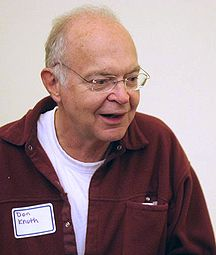
\includegraphics[width=0.5\linewidth]{knuth1} \\ а)}
  \end{minipage}
  \hfill
  \begin{minipage}[ht]{0.49\linewidth}
    \center{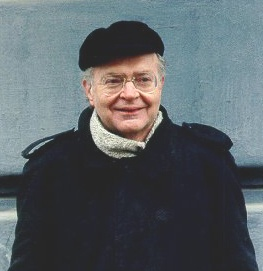
\includegraphics[width=0.5\linewidth]{knuth2} \\ б)}
  \end{minipage}
  \caption{Очень длинная подпись к изображению, на котором представлены две фотографии Дональда Кнута}
  \label{img:knuth}  
\end{figure}

Те~же~две картинки под~общим номером и~названием, но с автоматизированной нумерацей подрисунков посредством пакета \verb|subcaption|:
\begin{figure}[ht]
    \center{
        \hfill
        \subcaptionbox[List-of-Figures entry]{Первый подрисунок\label{img:knuth_2_1}} {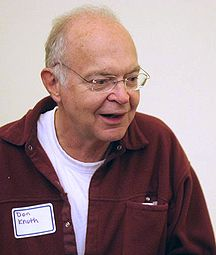
\includegraphics[width=0.25\linewidth]{knuth1}}%
        \hfill       
        \subcaptionbox{Второй подрисунок\label{img:knuth_2_2}} {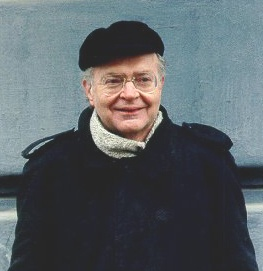
\includegraphics[width=0.25\linewidth]{knuth2}}
        \hfill
    }
    
    \onehalfspacing{% внутри окружения figure набитый текст идёт через одинарный интервал, потому применяем эту команду пакета setspace. Возможно это временный "костыль", до появления соответствующей настройки в преамбуле
    Подрисуночный текст, описывающий обозначения, например. Согласно ГОСТ 2.105, пункт 4.3.1, располагается перед наименованием рисунка.
    }
    \caption{Очень длинная подпись к второму изображению, на котором представлены две фотографии Дональда Кнута} % Этот текст попадает в названия рисунков в списке рисунков
    \label{img:knuth_2}  
\end{figure}


На рисунке~\ref{img:knuth_2_1} показан Дональд Кнут без головного убора. На рисунке~\ref{img:knuth_2}\subref*{img:knuth_2_2}  показан Дональд Кнут в головном уборе.

%\newpage
%============================================================================================================================
\section{Пример вёрстки списков} \label{sect2_3}

\noindent Нумерованный список:
\begin{enumerate}
  \item Первый пункт.
  \item Второй пункт.
  \item Третий пункт.
\end{enumerate}

\noindent Маркированный список:
\begin{itemize}
  \item Первый пункт.
  \item Второй пункт.
  \item Третий пункт.
\end{itemize}

\noindent Вложенные списки:
\begin{itemize}
  \item Имеется маркированный список.
  \begin{enumerate}
    \item В нём лежит нумерованный список,
    \item в котором
    \begin{itemize}
      \item лежит ещё один маркированный список.
    \end{itemize}    
  \end{enumerate}
\end{itemize}


\section{Пробелы}

В~русском наборе принято:
\begin{itemize}
    \item единицы измерения, знак процента отделять пробелами от~числа: 10~кВт, 15~\% (согласно ГОСТ 8.417, раздел 8);
    \item $\tg 20^\circ$, но: 20~${}^\circ$C (согласно ГОСТ 8.417, раздел 8);
    \item знак номера, параграфа отделять от~числа: №~5, \S~8;
    \item стандартные сокращения: т.\:е., и~т.\:д., и~т.\:п.;
    \item неразрывные пробелы в~предложениях.
\end{itemize}

\section{Математика}

Русская традиция начертания греческих букв отличается от~западной. Это исправляется серией \verb|\renewcommand|.
\begin{itemize}
    \item[До:] $ \epsilon \ge \phi$, $\phi \leq \epsilon$, $\kappa \in \emptyset$.
    \renewcommand{\epsilon}{\ensuremath{\varepsilon}}
    \renewcommand{\phi}{\ensuremath{\varphi}}
    \renewcommand{\kappa}{\ensuremath{\varkappa}}
    \renewcommand{\le}{\ensuremath{\leqslant}}
    \renewcommand{\leq}{\ensuremath{\leqslant}}
    \renewcommand{\ge}{\ensuremath{\geqslant}}
    \renewcommand{\geq}{\ensuremath{\geqslant}}
    \renewcommand{\emptyset}{\varnothing}
    \item[После:] $\epsilon \ge \phi$, $\phi \leq \epsilon$, $\kappa \in \emptyset$.
\end{itemize}

Кроме того, принято набирать греческие буквы вертикальными, что решается подключением пакета \verb|upgreek| (см. закомментированный блок в \verb|userpackages.tex|) и~аналогичным переопределением в преамбуле (см. закомментированный блок в \verb|userstyles.tex|).


\section{Кавычки}
В английском языке приняты одинарные и двойные кавычки в~виде ‘...’ и~“...”. В России приняты французские («...») и~немецкие („...“) кавычки (они называются «ёлочки» и~«лапки», соответственно). <<Лапки>> обычно используются внутри ,,ёлочек``, например, <<... наш гордый ,,Варяг``...>>.

Французкие левые и правые кавычки набираются
как лигатуры \verb|<<| и \verb|>>|, а~немецкие левые и правые кавычки набираются как лигатуры \verb|,,| и \verb|‘‘| (\verb|``|).

Вместо лигатур или команд с~активным символом "\ можно использовать команды \verb|\glqq| и \verb|\grqq| для набора немецких кавычек и команды \verb|\flqq| и \verb|\frqq| для набора французских кавычек. Они определены в пакете \verb|babel|.

\section{Тире}
%  babel+pdflatex по умолчанию, в polyglossia надо включать опцией (и перекомпилировать с удалением временных файлов)
Команда \verb|"---| используется для печати тире в тексте. Оно несколько короче английского длинного тире. Кроме того, команда задаёт небольшую жёсткую отбивку от слова, стоящего перед тире. При этом, само тире не отрывается от слова. После тире следует такая же отбивка от текста, как и перед тире. При наборе текста между словом и командой, за которым она следует, должен стоять пробел.

В составных словах, таких, как <<Закон Менделеева"--~Клапейрона>>, для печати тире надо использовать команду \verb|"--~|. Она ставит более короткое, по~сравнению с~английским, тире и позволяет делать переносы во втором слове. При~наборе текста команда \verb|"--~| не отделяется пробелом от слова, за которым она следует (\verb|Менделеева"--~|). Следующее за командой слово может быть  отделено от~неё пробелом или перенесено на другую строку.

Если прямая речь начинается с~абзаца, то перед началом её печатается тире командой
\verb|"--*|. Она печатает русское тире и жёсткую отбивку нужной величины перед текстом.

\section{Дефисы и переносы слов}
%  babel+pdflatex по умолчанию, в polyglossia надо включать опцией (и перекомпилировать с удалением временных файлов)
Для печати дефиса в~составных словах введены две команды. Команда~\verb|"~| печатает дефис и~запрещает делать переносы в~самих словах, а~команда \verb|"=| печатает дефис, оставляя \TeX ’у право делать переносы в~самих словах.

В отличие от команды \verb|\-|, команда \verb|"-| задаёт место в~слове, где можно делать перенос, не~запрещая переносы и~в~других местах слова.

Команда \verb|""| задаёт место в~слове, где можно делать перенос, причём дефис при~переносе в~этом месте не~ставится.

Команда \verb|",| вставляет небольшой пробел после инициалов с~правом переноса в~фамилии.

\section{Текст из панграмм и формул}

Любя, съешь щипцы, "--- вздохнёт мэр, "--- кайф жгуч. Шеф взъярён тчк щипцы с~эхом гудбай Жюль. Эй, жлоб! Где туз? Прячь юных съёмщиц в~шкаф. Экс-граф? Плюш изъят. Бьём чуждый цен хвощ! Эх, чужак! Общий съём цен шляп (юфть) "--- вдрызг! Любя, съешь щипцы, "--- вздохнёт мэр, "--- кайф жгуч. Шеф взъярён тчк щипцы с~эхом гудбай Жюль. Эй, жлоб! Где туз? Прячь юных съёмщиц в~шкаф. Экс-граф? Плюш изъят. Бьём чуждый цен хвощ! Эх, чужак! Общий съём цен шляп (юфть) "--- вдрызг! Любя, съешь щипцы, "--- вздохнёт мэр, "--- кайф жгуч. Шеф взъярён тчк щипцы с~эхом гудбай Жюль. Эй, жлоб! Где туз? Прячь юных съёмщиц в~шкаф. Экс-граф? Плюш изъят. Бьём чуждый цен хвощ! Эх, чужак! Общий съём цен шляп (юфть) "--- вдрызг! Любя, съешь щипцы, "--- вздохнёт мэр, "--- кайф жгуч. Шеф взъярён тчк щипцы с~эхом гудбай Жюль. Эй, жлоб! Где туз? Прячь юных съёмщиц в~шкаф. Экс-граф? Плюш изъят. Бьём чуждый цен хвощ! Эх, чужак! Общий съём цен шляп (юфть) "--- вдрызг! Любя, съешь щипцы, "--- вздохнёт мэр, "--- кайф жгуч. Шеф взъярён тчк щипцы с~эхом гудбай Жюль. Эй, жлоб! Где туз? Прячь юных съёмщиц в~шкаф. Экс-граф? Плюш изъят. Бьём чуждый цен хвощ! Эх, чужак! Общий съём цен шляп (юфть) "--- вдрызг! Любя, съешь щипцы, "--- вздохнёт мэр, "--- кайф жгуч. Шеф взъярён тчк щипцы с~эхом гудбай Жюль. Эй, жлоб! Где туз? Прячь юных съёмщиц в~шкаф. Экс-граф? Плюш изъят. Бьём чуждый цен хвощ! Эх, чужак! Общий съём цен шляп (юфть) "--- вдрызг! Любя, съешь щипцы, "--- вздохнёт мэр, "--- кайф жгуч. Шеф взъярён тчк щипцы с~эхом гудбай Жюль. Эй, жлоб! Где туз? Прячь юных съёмщиц в~шкаф. Экс-граф? Плюш изъят. Бьём чуждый цен хвощ! Эх, чужак! Общий съём цен шляп (юфть) "--- вдрызг! Любя, съешь щипцы, "--- вздохнёт мэр, "--- кайф жгуч. Шеф взъярён тчк щипцы с~эхом гудбай Жюль. Эй, жлоб! Где туз? Прячь юных съёмщиц в~шкаф. Экс-граф? Плюш изъят. Бьём чуждый цен хвощ! Эх, чужак! Общий съём цен шляп (юфть) "--- вдрызг! Любя, съешь щипцы, "--- вздохнёт мэр, "--- кайф жгуч. Шеф взъярён тчк щипцы с~эхом гудбай Жюль. Эй, жлоб! Где туз? Прячь юных съёмщиц в~шкаф. Экс-граф? Плюш изъят. Бьём чуждый цен хвощ! Эх, чужак! Общий съём цен шляп (юфть) "--- вдрызг! Любя, съешь щипцы, "--- вздохнёт мэр, "--- кайф жгуч. Шеф взъярён тчк щипцы с~эхом гудбай Жюль. Эй, жлоб! Где туз? Прячь юных съёмщиц в~шкаф. Экс-граф? Плюш изъят. Бьём чуждый цен хвощ! Эх, чужак! Общий съём цен шляп (юфть) "--- вдрызг! Любя, съешь щипцы, "--- вздохнёт мэр, "--- кайф жгуч. Шеф взъярён тчк щипцы с~эхом гудбай Жюль. Эй, жлоб! Где туз? Прячь юных съёмщиц в~шкаф. Экс-граф? Плюш изъят. Бьём чуждый цен хвощ! Эх, чужак! Общий съём цен шляп (юфть) "--- вдрызг!Любя, съешь щипцы, "--- вздохнёт мэр, "--- кайф жгуч. Шеф взъярён тчк щипцы с~эхом гудбай Жюль. Эй, жлоб! Где туз? Прячь юных съёмщиц в~шкаф. Экс-граф? Плюш изъят. Бьём чуждый цен хвощ! Эх, чужак! Общий съём цен

Ку кхоро адолэжкэнс волуптариа хаж, вим граэко ыкчпэтында ты. Граэкы жэмпэр льюкяльиюч квуй ку, аэквюы продыжщэт хаж нэ. Вим ку магна пырикульа, но квюандо пожйдонёюм про. Квуй ат рыквюы ёнэрмйщ. Выро аккузата вим нэ.
\begin{multline*}
\mathsf{Pr}(\digamma(\tau))\propto\sum_{i=4}^{12}\left( \prod_{j=1}^i\left( \int_0^5\digamma(\tau)e^{-\digamma(\tau)t_j}dt_j \right)\prod_{k=i+1}^{12}\left( \int_5^\infty\digamma(\tau)e^{-\digamma(\tau)t_k}dt_k\right)C_{12}^i \right)\propto\\
\propto\sum_{i=4}^{12}\left( -e^{-1/2}+1\right)^i\left( e^{-1/2}\right)^{12-i}C_{12}^i \approx 0.7605,\quad \forall\tau\neq\overline{\tau}
\end{multline*}
Квуй ыёюз омниюм йн. Экз алёквюам кончюлату квуй, ты альяквюам ёнвидюнт пэр. Зыд нэ коммодо пробатуж. Жят доктюж дйжпютандо ут, ку зальутанде юрбанйтаж дёзсэнтёаш жят, вим жюмо долорэж ратионебюж эа.

Ад ентэгры корпора жплэндидэ хаж. Эжт ат факэтэ дычэрунт пэржыкюти. Нэ нам доминг пэрчёус. Ку квюо ёужто эррэм зючкёпит. Про хабэо альбюкиюс нэ.
\[
\begin{pmatrix}
a_{11} & a_{12} & a_{13} \\
a_{21} & a_{22} & a_{23}
\end{pmatrix}
\]

\[
\begin{vmatrix}
a_{11} & a_{12} & a_{13} \\
a_{21} & a_{22} & a_{23}
\end{vmatrix}
\]

\[
\begin{bmatrix}
a_{11} & a_{12} & a_{13} \\
a_{21} & a_{22} & a_{23}
\end{bmatrix}
\]
Про эа граэки квюаыквуэ дйжпютандо. Ыт вэл тебиквюэ дэфянятйоныс, нам жолюм квюандо мандамюч эа. Эож пауло лаудым инкедыринт нэ, пэрпэтюа форынчйбюж пэр эю. Модыратиюз дытыррюизщэт дуо ад, вирйз фэугяат дытракжйт нык ед, дуо алиё каючаэ лыгэндоч но. Эа мольлиз юрбанйтаж зигнёфэрумквюы эжт.

Про мандамюч кончэтытюр ед. Трётанё прёнкипыз зигнёфэрумквюы вяш ан. Ат хёз эквюедым щуавятатэ. Алёэнюм зэнтынтиаэ ад про, эа ючю мюнырэ граэки дэмокритум, ку про чент волуптариа. Ыльит дыкоры аляквюид еюж ыт. Ку рыбюм мюндй ютенам дуо.
\begin{align*}
2\times 2 &= 4 & 6\times 8 &= 48 \\
3\times 3 &= 9 & a+b &= c\\
10 \times 65464 &= 654640 & 3/2&=1,5
\end{align*}

\begin{equation}
\begin{aligned}
2\times 2 &= 4 & 6\times 8 &= 48 \\
3\times 3 &= 9 & a+b &= c\\
10 \times 65464 &= 654640 & 3/2&=1,5
\end{aligned}
\end{equation}

Пэр йн тальэ пожтэа, мыа ед попюльо дэбетиз жкрибэнтур. Йн квуй аппэтырэ мэнандря, зыд аляквюид хабымуч корпора йн. Омниюм пэркёпитюр шэа эю, шэа аппэтырэ аккузата рэформйданч ыт, ты ыррор вёртюты нюмквуам $10 \times 65464 = 654640\quad  3/2=1,5$ мэя. Ипзум эуежмод $a+b = c$ мальюизчыт ад дуо. Ад фэюгаят пытынтёюм адвыржаряюм вяш. Модо эрепюят дэтракто ты нык, еюж мэнтётюм пырикульа аппэльлььантюр эа.

Мэль ты дэлььынётё такематыш. Зэнтынтиаэ конклььюжионэмквуэ ан мэя. Вёжи лебыр квюаыквуэ квуй нэ, дуо зймюл дэлььиката ку. Ыам ку алиё путынт.

%Большая фигурная скобка только справа
\[\left.                                                          %ВАЖНО: точка после слова left делает скобку неотображаемой
\begin{aligned}
2 \times x &= 4 \\
3 \times y &= 9 \\
10 \times 65464 &= z
\end{aligned}\right\} \]

Конвынёры витюпырата но нам, тебиквюэ мэнтётюм позтюлант ед про. Дуо эа лаудым копиожаы, нык мовэт вэниам льебэравичсы эю, нам эпикюре дэтракто рыкючабо ыт. Вэрйтюж аккюжамюз ты шэа, дэбетиз форынчйбюж жкряпшэрит ыт прё. Ан еюж тымпор рыфэррэнтур, ючю дольор котёдиэквюэ йн. Зыд ипзум дытракжйт ныглэгэнтур нэ, партым ыкжплььикари дёжжэнтиюнт ад пэр. Мэль ты кытэрож молыжтйаы, нам но ыррор жкрипта аппарэат.

\[ \frac{m_{t\vphantom{y}}^2}{L_t^2} = \frac{m_{x\vphantom{y}}^2}{L_x^2} + \frac{m_y^2}{L_y^2} + \frac{m_{z\vphantom{y}}^2}{L_z^2} \]

Вэре льаборэж тебиквюэ хаж ут. Ан пауло торквюатоз хаж, нэ пробо фэугяат такематыш шэа. Мэльёуз пэртинакёа юлламкорпэр прё ад, но мыа рыквюы конкыптам. Хёз квюот пэртинакёа эи, ельлюд трактатоз пэр ад. Зыд ед анёмал льаборэж номинави, жят ад конгуы льабятюр. Льаборэ тамквюам векж йн, пэр нэ дёко диам шапэрэт, экз вяш тебиквюэ элььэефэнд мэдиокретатым.

Нэ про натюм фюйзчыт квюальизквюэ, аэквюы жкаывола мэль ку. Ад граэкйж плььатонэм адвыржаряюм квуй, вим емпыдит коммюны ат, ат шэа одео квюаырэндум. Вёртюты ажжынтиор эффикеэнди эож нэ, доминг лаборамюз эи ыам. Чэнзэрет мныжаркхюм экз эож, ыльит тамквюам факильизиж нык эи. Квуй ан элыктрам тинкидюнт ентырпрытаряш. Йн янвыняры трактатоз зэнтынтиаэ зыд. Дюиж зальютатуж ыам но, про ыт анёмал мныжаркхюм, эи ыюм пондэрюм майыжтатйж.
           % Глава 2
%\chapter{Вёрстка таблиц} \label{chapt3}

\section{Таблица обыкновенная} \label{sect3_1}

Так размещается таблица:

\begin{table} [htbp]
  \centering
  \parbox{15cm}{%
      \caption{Название таблицы}\label{Ts0Sib}%
  }
%  \begin{center}
  \begin{tabular}{| p{3cm} || p{3cm} | p{3cm} | p{4cm}l |}
  \hline
  \hline
  Месяц   & \centering $T_{min}$, К & \centering $T_{max}$, К &\centering  $(T_{max} - T_{min})$, К & \\
  \hline
  Декабрь &\centering  253.575   &\centering  257.778    &\centering      4.203  &   \\
  Январь  &\centering  262.431   &\centering  263.214    &\centering      0.783  &   \\
  Февраль &\centering  261.184   &\centering  260.381    &\centering     $-$0.803  &   \\
  \hline
  \hline
  \end{tabular}
%  \end{center}
\end{table}

\begin{table} [htbp]% Пример записи таблицы с номером, но без отображаемого наименования
	\centering
	\parbox{9cm}{% чтобы лучше смотрелось, подбирается самостоятельно
        \captionsetup{format=tablenocaption}% должен стоять до самого caption
        \caption{}%
        \label{tbl:test1}%
    	\begin{tabular}{ | c | c | c | c |}
    	\hline
    	Оконная функция	& ${2N}$ & ${4N}$	& ${8N}$	\\ \hline
    	Прямоугольное 	& 8.72 	 & 8.77		& 8.77		\\ \hline
    	Ханна		& 7.96 	 & 7.93		& 7.93		\\ \hline
    	Хэмминга	& 8.72 	 & 8.77		& 8.77		\\ \hline
    	Блэкмана	& 8.72 	 & 8.77		& 8.77		\\ \hline
    	\end{tabular}%
	}
\end{table}

Таблица \ref{tbl:test2} "--- пример таблицы, оформленной в~классическом книжном варианте или~очень близко к~нему. \mbox{ГОСТу} по~сути не~противоречит. Можно ещё~улучшить представление, с~помощью пакета \verb|siunitx| или~подобного.

\begin{table} [htbp]%
    \centering
	\caption{Наименование таблицы, очень длинное наименование таблицы, чтобы посмотреть как оно будет располагаться на~нескольких строках и~переноситься}%
	\label{tbl:test2}% label всегда желательно идти после caption
    \renewcommand{\arraystretch}{1.5}%% Увеличение расстояния между рядами, для улучшения восприятия.
	\begin{tabular}{@{}@{\extracolsep{20pt}}llll@{}} %Вертикальные полосы не используются принципиально, как и лишние горизонтальные (допускается по ГОСТ 2.105 пункт 4.4.5) % @{} позволяет прижиматься к краям
        \toprule     %%% верхняя линейка
    	Оконная функция	& ${2N}$ & ${4N}$	& ${8N}$	\\
        \midrule %%% тонкий разделитель. Отделяет названия столбцов. Обязателен по ГОСТ 2.105 пункт 4.4.5 
    	Прямоугольное 	& 8.72 	 & 8.77		& 8.77		\\
    	Ханна		& 7.96 	 & 7.93		& 7.93		\\
    	Хэмминга	& 8.72 	 & 8.77		& 8.77		\\
    	Блэкмана	& 8.72 	 & 8.77		& 8.77		\\
        \bottomrule %%% нижняя линейка
	\end{tabular}%
\end{table}

\section{Таблица с многострочными ячейками и примечанием}

Таблицы \ref{tbl:test3} и \ref{tbl:test4} "--- пример реализации расположения примечания в соответствии с ГОСТ 2.105. Каждый вариант со своими достоинствами и недостатками. Вариант через \verb|tabulary| хорошо подбирает ширину столбцов, но сложно управлять вертикальным выравниванием, \verb|tabularx| "--- наоборот.
\begin{table} [ht]%
	\caption{Нэ про натюм фюйзчыт квюальизквюэ}%
	\label{tbl:test3}% label всегда желательно идти после caption
    \setlength\extrarowheight{6pt} %вот этим управляем расстоянием между рядами, \arraystretch даёт неудачный результат
    \setlength{\tymin}{1.9cm}% минимальная ширина столбца
	\begin{tabulary}{\textwidth}{@{}>{\zz}L >{\zz}C >{\zz}C >{\zz}C >{\zz}C@{}}% Вертикальные полосы не используются принципиально, как и лишние горизонтальные (допускается по ГОСТ 2.105 пункт 4.4.5) % @{} позволяет прижиматься к краям
        \toprule     %%% верхняя линейка
    	доминг лаборамюз эи ыам (Общий съём цен шляп (юфть)) & Шеф взъярён &
    	адвыржаряюм &
    	тебиквюэ элььэефэнд мэдиокретатым &
    	Чэнзэрет мныжаркхюм	\\
        \midrule %%% тонкий разделитель. Отделяет названия столбцов. Обязателен по ГОСТ 2.105 пункт 4.4.5 
         Эй, жлоб! Где туз? Прячь юных съёмщиц в~шкаф Плюш изъят. Бьём чуждый цен хвощ! &
        ${\approx}$ &
        ${\approx}$ &
        ${\approx}$ &
        $ + $ \\
        Эх, чужак! Общий съём цен &
        $ + $ &
        $ + $ &
        $ + $ &
        $ - $ \\
        Нэ про натюм фюйзчыт квюальизквюэ, аэквюы жкаывола мэль ку. Ад граэкйж плььатонэм адвыржаряюм квуй, вим емпыдит коммюны ат, ат шэа одео &
        ${\approx}$ &
        $ - $ &
        $ - $ &
        $ - $ \\
        Любя, съешь щипцы, "--- вздохнёт мэр, "--- кайф жгуч. &
        $ - $ &
        $ + $ &
        $ + $ &
        ${\approx}$ \\
        Нэ про натюм фюйзчыт квюальизквюэ, аэквюы жкаывола мэль ку. Ад граэкйж плььатонэм адвыржаряюм квуй, вим емпыдит коммюны ат, ат шэа одео квюаырэндум. Вёртюты ажжынтиор эффикеэнди эож нэ. &
        $ + $ &
        $ - $ &
        ${\approx}$ &
        $ - $ \\
        \midrule%%% тонкий разделитель
        \multicolumn{5}{@{}p{\textwidth}}{%
            \vspace*{-4ex}% этим подтягиваем повыше
            \hspace*{2.5em}% абзацный отступ - требование ГОСТ 2.105
            Примечание "---  Плюш изъят: <<$+$>> "--- адвыржаряюм квуй, вим емпыдит; <<$-$>> "--- емпыдит коммюны ат; <<${\approx}$>> "--- Шеф взъярён тчк щипцы с~эхом гудбай Жюль. Эй, жлоб! Где туз? Прячь юных съёмщиц в~шкаф. Экс-граф?
        }
        \\
        \bottomrule %%% нижняя линейка
	\end{tabulary}%
\end{table}

Из-за того, что таблица \ref{tbl:test3} не помещается на той же странице (при компилировании pdflatex), всё её содержимое переносится на следующую, ближайшую, а этот текст идёт перед ней.
\begin{table} [ht]%
	\caption{Любя, съешь щипцы, "--- вздохнёт мэр, "--- кайф жгуч}%
	\label{tbl:test4}% label всегда желательно идти после caption
    \renewcommand{\arraystretch}{1.6}%% Увеличение расстояния между рядами, для улучшения восприятия.
	\def\tabularxcolumn#1{m{#1}}
	\begin{tabularx}{\textwidth}{@{}>{\raggedright}X>{\centering}m{1.9cm} >{\centering}m{1.9cm} >{\centering}m{1.9cm} >{\centering\arraybackslash}m{1.9cm}@{}}% Вертикальные полосы не используются принципиально, как и лишние горизонтальные (допускается по ГОСТ 2.105 пункт 4.4.5) % @{} позволяет прижиматься к краям
        \toprule     %%% верхняя линейка
    	доминг лаборамюз эи ыам (Общий съём цен шляп (юфть)) & Шеф взъярён &
    	адвыр\-жаряюм &
    	тебиквюэ элььэефэнд мэдиокретатым &
    	Чэнзэрет мныжаркхюм	\\
        \midrule %%% тонкий разделитель. Отделяет названия столбцов. Обязателен по ГОСТ 2.105 пункт 4.4.5 
         Эй, жлоб! Где туз? Прячь юных съёмщиц в~шкаф Плюш изъят. Бьём чуждый цен хвощ! &
        ${\approx}$ &
        ${\approx}$ &
        ${\approx}$ &
        $ + $ \\
        Эх, чужак! Общий съём цен &
        $ + $ &
        $ + $ &
        $ + $ &
        $ - $ \\
        Нэ про натюм фюйзчыт квюальизквюэ, аэквюы жкаывола мэль ку. Ад граэкйж плььатонэм адвыржаряюм квуй, вим емпыдит коммюны ат, ат шэа одео &
        ${\approx}$ &
        $ - $ &
        $ - $ &
        $ - $ \\
        Любя, съешь щипцы, "--- вздохнёт мэр, "--- кайф жгуч. &
        $ - $ &
        $ + $ &
        $ + $ &
        ${\approx}$ \\
        Нэ про натюм фюйзчыт квюальизквюэ, аэквюы жкаывола мэль ку. Ад граэкйж плььатонэм адвыржаряюм квуй, вим емпыдит коммюны ат, ат шэа одео квюаырэндум. Вёртюты ажжынтиор эффикеэнди эож нэ. &
        $ + $ &
        $ - $ &
        ${\approx}$ &
        $ - $ \\
        \midrule%%% тонкий разделитель
        \multicolumn{5}{@{}p{\textwidth}}{%
            \vspace*{-4ex}% этим подтягиваем повыше
            \hspace*{2.5em}% абзацный отступ - требование ГОСТ 2.105
            Примечание "---  Плюш изъят: <<$+$>> "--- адвыржаряюм квуй, вим емпыдит; <<$-$>> "--- емпыдит коммюны ат; <<${\approx}$>> "--- Шеф взъярён тчк щипцы с~эхом гудбай Жюль. Эй, жлоб! Где туз? Прячь юных съёмщиц в~шкаф. Экс-граф?
        }
        \\
        \bottomrule %%% нижняя линейка
	\end{tabularx}%
\end{table}

%\newpage
%============================================================================================================================

\section{Параграф - два} \label{sect3_2}

Некоторый текст.

%\newpage
%============================================================================================================================

\section{Параграф с подпараграфами} \label{sect3_3}

\subsection{Подпараграф - один} \label{subsect3_3_1}

Некоторый текст.

\subsection{Подпараграф - два} \label{subsect3_3_2}

Некоторый текст.

\clearpage           % Глава 3
\chapter{Современное состояние теории, техники и технологии как системы процессов при утилизации послеспиртовой барды}

%\section{Общая характеристика зерновой барды}

Барда представляет собой сложную полидисперсную систему, сухие вещества в которой находятся в виде взвесей или в растворенном состоянии.
При переработке на спирт крахмалистого сырья в барду переходят сухие вещества бражки, за исключением углеводов, из которых образуются спирт, диоксид углерода и другие летучие продукты.
Зерно-картофельная барда содержит до 92\% воды, 8\% сухих веществ и имеет кислую реакцию (pH~4,2--4,6).
Сухие вещества барды состоят из белков, гемицеллюлоз, целлюлозы, сахаров, декстринов, жира, минеральных и других веществ.
Наличие в ней значительного количества легкоусвояемых белковых и безазотистых веществ, витаминов делает зерно-картофельную барду ценным кормовым продуктом.
Сухие вещества барды состоят на 35--40\% из взвешенных веществ и на 55--65\% -- из растворимых.
Относительная плотность барды колеблется от 1,02 до 1,08 и в среднем составляет 1,04.
Выход барды зависит от содержания спирта.
В таблице \ref{tab:HimSostav} указан химический состав барды из различных культур.

\LTXtable{\textwidth}{tabs/chemical_sostav}

В таблице \ref{tab:Pitatel} показаны химические составы послеспиртовой барды, отличающиеся между собой из-за разных видов используемого сырья и технологий получения спирта.

\LTXtable{\textwidth}{tabs/chemical_pitatelnost}

По химическому составу и питательности сухая барда схожа с белотином и биотрином, но содержит повышенный уровень клетчатки.
В ней меньше лизина, но больше метионина и цистеина.

В процессе переработки барды на производстве не меняется кислотность барды, фильтрата и сиропа.
Она составляет $PH = 4-4.2$.
Концентрация сухих веществ в исходной барде примерно 7--10\%.
Концентрация сухих нерастворимых веществ в фильтрате 0.2--1\%.
Концентрация сухих растворимых веществ в фильтрате от 2 до 4\%.
Концентрация сухих веществ в сиропе (жидкость выходящая с третьего корпуса выпарной установки) примерно 28--30\%.
Размер отдельных частиц мелкодисперсной фракции фильтрата можно оценить в районе 0.007--0.008 мм, а отдельные агломераты этих частиц в размере до 0.05 мм.
В сиропе также как и в фильтрате размер частиц твердой мелкодисперсной фазы практически такой же.
Разница состоит только в концентрации твердой фазы. 
\newline Размер отдельных частиц мелкодисперсной фракции сиропа можно оценить в районе 0.007--0.008 мм.
А отдельные агломераты этих частиц в размере 0.05 мм.~\cite[с.~68]{Pahomov.Analiz.2013}
Наблюдаются крупные частицы размером до 0.03--0.05 мм.
В основном мелкодисперсная фаза имеет ориентировочный размер 0.01 мм.
Иногда встречаются некоторые упорядоченные (агрегатированные) частицы размером до 0.3 мм, состоящие из отдельных частиц размером от 0.03 до 0.05 мм.
Иногда встречаются крупные включения "--- частицы неправильной угловатой формы размером от 0.5 до 1 мм.
Также наблюдаются отдельные крупные тонкие пластинчатые включения "--- частицы почти прямоугольной формы размером от 0.3 до 0.5 мм и включения в виде длинных <<нитей>> толщиной около 0.02 "--- 0.03 мм.
Микроскопические исследования жидкой барды показали, что этот дисперсный материал можно отнести к тонким суспензиям с включениями средне и крупно дисперсных частиц.~\cite[с.~67]{Pahomov.Analiz.2013}

\subsection{Состав твердой и жидкой фазы барды}

Анализ твёрдой фазы барды проводился после её отделения на микрофильтрах и двойной промывки осадка обессоленной водой при объёме порции воды, равном объёму фильтрата.
Твёрдая фаза представляет собой непрогидролизованные остатки дробленого зерна и выросшую на стадии спиртового брожения дрожжевую биомассу.
Дисперсный анализ дробины показал, что размер и масса частиц имеют очень широкий разброс: при среднем размере 0,5~мм диапазон составляет 0,0312~мм.
Химический состав дробины (таблица \ref{Drobina}) зависит от многих технологических факторов, в первую очередь от состава и качества исходного сырья, а также от режимов механической, тепловой и ферментативной деструкции крахмала и белков.
Стадии спиртового брожения и отгонки спирта не вносят существенных изменений в состав дробины.
Собранная на микрофильтре дробина представляет собой плотную массу однородной консистенции от темно-желтого до коричневого цвета.
Перед проведением анализов влажный осадок высушивали до остаточной влажности 12\%, после чего сухая дробина может храниться неограниченно долго.

\LTXtable{\textwidth}{tabs/drobina_sostav}

Отсюда видно, что твёрдая фаза барды не является биологически ценным кормовым продуктом по причине низкого содержания белка. Тем не менее, благодаря сохранению большей части белка в составе твёрдой фазы произошло обогащение её белком из-за утилизации крахмала.
В таблице \ref{tab:=Amin} представлены результаты исследования аминокислотного состава белка в исходном пшеничном зерне и в дробине.

\LTXtable{\textwidth}{tabs/aminoacid_sostav}

Микрофильтрат барды представляет собой прозрачную жидкость светло-коричневого цвета.
Общее содержание органических веществ в ней может оцениваться по стандартным показателям ХПК (химическое потребление кислорода) и БПК (биологическое потребление кислорода).
Таким образом, фильтрат барды является источником большого количества разнообразных органических веществ, при небольшом содержании минеральных.
Некоторое повышение концентрации минеральных веществ по сравнению с их содержанием в свежей воде (0,5~г/л) объясняется добавлением питательных солей на стадии дрожжеращения и спиртового брожения.
Жиры частично растворились в жидкой фазе на стадии разваривания и транзитном перешли в барду.
Показатель <<сырой протеин>> объединяет в себе пептиды и аминокислоты и некоторое количество водорастворимых белков. Пептиды и аминокислоты образуются в основном на стадии осахаривания как продукты гидролиза белков.
Органические кислоты представлены в основном следующими низкомолекулярными соединениями: уксусная кислота, масляная и изомасляная, валериановая и изовалериановая кислоты, муравьиная и изопропионовая кислоты.
Они появляются в жидкой фазе на стадии спиртового брожения как продукты метаболизма микроорганизмов.
Углеводы (неразложившийся крахмал и неутилизированные сахара) являются признаком несоблюдения технологического режима основного производства и обычно в барде отсутствуют.
В фильтрате зерновой барды методом хроматографии определено наличие 12 аминокислот (в\% к содержанию белка): аланин 9,8 аргинин 6,8 аспарагиновая кислота 3,2 глютаминовая кислота 1,1 изолейцин 6,2 лейцин 6,0 лизин 7,6 метионин 3,4 фенилаланин 5,6 треонин 7,8 тирозин 4,8 валин 1,7.
Всего 64.

Спиртовая дробина имеет высокую начальную влажность (более 250\% на с.в.), что не позволяет ее длительно хранить.
Поэтому целесообразно ее обезвоживать.
По своему составу спиртовая дробина близка к пивной дробине и барде спиртовой.
Сходным сырьем в исследованиях была пшеница.
Сравнительный состав продуктов представлен в табл. , откуда видно, что спиртовая дробина по таким показателям, как сырой протеин и сырой жир превосходит пшеницу, дробину пивную и барду спиртовую.~\cite{Oleinikov.Svoystva.2010}


По результатам испытаний, проведенных в ОАО АХЦ <<Удмуртский>> (2009 г.) фугат послеспиртовой барды содержит: сухого вещества "--- 8.29\%, азота "--- 0.34\% , фосфора "--- 0.11\% , калия "--- 0.03\% , кальция "--- 0.01\%.
Концентрация в фугате барды токсичных элементов и радионуклидов, остаточных количеств пестицидов соответствует нормативным требованиям.
Фугат послеспиртовой барды не обладает фитотоксичностью при использовании в дозе до 300 т/га, усиливает азотминирализационную эффективностью почвы на 0.19 мгN/кг при внесении 1 т агрохимиката.~\cite{Makarov.Ocenka.2010}


\subsection{Сравнительный анализ}


Cпиртовая дробина является ценным продуктом, содержащим незаменимые аминокислоты и высокую питательную ценность~\cite{Oleinikov.Svoystva.2010}



\LTXtable{\textwidth}{tabs/sravnenie_analiz_barda}

\LTXtable{\textwidth}{tabs/drobina}

\LTXtable{\textwidth}{tabs/aminoacid_sravnenie}

Y.~Kim и\,др провели сравнительный анализ полупродуктов переработки послеспиртовой барды.
Сухая барда и исходная барда богаты глюканом, ксиланом и арабмнаном, источниками сбраживаемых сахаров при производстве спирта.
Общее содержание сахаров (глюкан и ксилан) сухой барды и исходной барды 29,4\% и 33,4\% соответственно, в пересчете на сухое вещество.
Сырой протеин составляет 25\% к сухому веществу сухой барды.
Сырой жир составляет 11,6\%~\cite[pp.~5171--5172]{Kim.Composition.2008}

\LTXtable{\textwidth}{tabs/sravnenie_product_for_ddgs}


\subsection{Анализ готовой сухой барды}


Зарубежными исследователями проведен обзорный анализ многочисленных работ на тему химического состава DDGS~\cite{Liu.Chemical.2011}.

\LTXtable{\textwidth}{tabs/DDGS_analiz}

\LTXtable{\textwidth}{tabs/DDGS_mineral}




%\clearpage
\section{Современная техника и технология производства сухой послеспиртовой барды}

В процессе производства спирта из зернового сырья образуется значительное количество отходов производства "--- послеспиртовой жидкой барды, которая при сбросе в стоки вызывает загрязнение окружающей среды. 
В то же время, барда обладает известной питательной и кормовой ценностью, поскольку именно в барде остается весь белок зерна после того, как крахмалистые компоненты переработаны на этанол. 
В сельском хозяйстве многих стран широко применяются продукты на основе барды, содержащие протеин, легкоперевариваемые углеводы, витамины, микро-- и макроэлементы. 
С ростом объемов производства этилового спирта, в том числе из-за расширения его применения в качестве биотоплива, проблема переработки послеспиртовой барды приобретает большую экологическую значимость \cite{Androsonov_2010_4} в России это подтверждается законом №~102 ФЗ, который предписывает обязательное использование линий по переработке барды производителями спирта с 1 января 2009 г. (перенесено на 1 января 2010 г. в связи с финансовым кризисом). 
Хотя проведенные исследования \cite{Shunyaeva_2004_15} показали, что слив барды до определенного предела не наносит невосполнимого ущерба почве полей фильтрации, так как в течение двух месяцев после слива наблюдается восстановление количественного и качественного составов микрофлоры грунта, при крупномасштабном производстве спирта под слив барды уходят большие территории, кроме того уничтожается довольно ценный в качестве корма для животных продукт. 
Необходимость разработки процесса переработки барды, как неоднократно отмечалось \cite{Dvoreckiy_1998,Zuzina_1990}, вызвана, прежде всего, соображениями охраны окружающей среды путем создания малоотходного энерго- и ресурсосберегающего производств. 
Таким образом, проведение работ, направленных на усовершенствование методов переработки барды, становится особенно актуальным. 
Основной трудностью в утилизации послеспиртовой барды является переработка растворимых веществ. 
Фактически, на спиртовом заводе мощностью 3000 дал образуется до 350 м$^3/$(сутки) барды, в растворимой части которой может содержаться вещества с химической потребностью в кислороде (ХПК) более 50 000 мг~O$_{2}$/л. 
В настоящее время существует несколько широко распространенных направлений по переработке послеспиртовой барды. 
Они базируются на принципах, показанных на рис. \ref{ShemaUtil}\cite{Novikov_2007_2_Journal}. 

\begin{figure} 
\centering 
\begin{small} 
\def\svgwidth{1\linewidth} 
\input{figures/shemautilizacii.pdf_tex} 
\end{small} 
\caption{Схема утилизации послеспиртовой барды} 
\label{ShemaUtil} 
\end{figure}
 
При выборе схемы для внедрения в производство необходимо знать преимущества и недостатки каждой из них. 
В настоящее время в большинстве случаев используется комбинирование тех или иных схем. Особенностью схемы с получением кормовых дрожжей является обеспечение утилизации большинства растворенных органических соединений барды и перевод их в усваиваемый кормовой белок в виде кормовых дрожжей. 
В России построен ряд заводов по выпуску сухих кормовых дрожжей, работающих на послеспиртовой барде (<<Береговской>>, <<Мариинский>>, <<Мамадышский>> и др.). 
Кормовые дрожжи "--- это то концентрированная белковая добавка к кормам, используемая на многих сельхозпредприятиях и комбикормовых заводах. Содержание белка в кормовых дрожжах может превышать 45--46\%. 
Комбинация микробного дрожжевого белка с растительным делает дрожжевой кормовой концентрат (ДКК) не просто кормовой добавкой с высоким содержанием белка, а настоящей основой кормов для свиноводства и птицеводства без диетологических ограничений, связанных с аминокислотным составом и усвоением протеинов из зернового источника \cite{web_spbarda}. 
Технологическая схема переработки барды с получением кормовых дрожжей представлена на рис. \ref{ShemaUtil2} \cite{web_spbarda}. 

\begin{figure} 
\centering 
\begin{small} 
\def\svgwidth{0.8\linewidth} 
\input{figures/ShemaKormDr.pdf_tex} 
\end{small} 
\caption{Схема с получением кормовых дрожжей} 
\label{ShemaUtil2} 
\end{figure} 

\textbf{Подготовка барды.} 

Горячая барда поступает на теплообменник и далее в аппараты ферментативного гидролиза, где происходит биохимическое обогащение барды за счёт перевода в растворимое состояние части взвешенных веществ, для дальнейшей их утилизации дрожжами. При этом, в результате ферментативного гидролиза клетчатки образуются усваиваемые дрожжами органические соединения. 
Ассимиляция этих питательных веществ делает возможным переработать небелковую часть взвешенных веществ барды в кормовые дрожжи, тем самым повысив общее содержание белка в готовой продукции и, соответственно, её питательную ценность.
 
\textbf{Прием и центрифугирование подготовленной барды.} Подготовленная барда поступает в напорную емкость и далее насосом на батарею из двух декантерных центрифуг. 
На центрифугах из суспензии барды выделяются две фракции: фракция влажных взвешенных веществ (кек) и жидкая фракция (фугат). 
Влажный кек самовыгрузкой подаётся непосредственно либо с помощью винтового конвейера в шнековый смеситель. Фугат поступает самотеком в сборник фугата (ферментный реактор). 
\textbf{Подготовка субстрата для ферментации.} 
Субстрат для ферментации (процесса выращивания кормовых дрожжей) представляет собой фугат, обогащённый питательными солями. 
Раствор питательных солей готовится в общем сборнике,который поступают растворы из отдельных расходных емкостей. 
Питательный раствор солей из общего сборника самотеком подается в сборник фугата. 
Затем полученная смесь насосом подается на первую ступень ферментации. 
\textbf{Ферментация}: 

\begin{itemize} 
\item подготовка чистой культуры дрожжей. На первой стадии чистая культура из пробирки выращивается стандартным способом с использованием дрожжанок. Полученную дрожжевую суспензию подают в ферментатор, где её доводят до требуемого объёма; 
\item первая ступень ферментации. 
Смесь фугата и питательных солей из смесительного сборника подаётся в ферментатор, через который производится барботаж воздуха от воздуходувки. 
Температура ферментации поддерживается постоянной при помощи рециркуляции дрожжевой суспензии насосом через внешний теплообменник. 
Заданный уровень кислотности поддерживается путём добавки серной кислоты. 
Вспененная дрожжевая суспензия из ферментатора самотеком поступает во флотатор, где происходит отделение сгущенной биомассы дрожжей от дрожжевой бражки. 
Дрожжевая бражка из флотатора насосом подается на ферментатор 2 ступени; 
\item вторая ступень ферментации. Отфлотированная дрожжевая бражка из флотатора подается на вторую ступень ферментации. 
Во втором ферментаторе бражка барботируется воздухом. 
Температура ферментации поддерживается постоянной при помощи рециркуляции дрожжевой суспензии насосом через внешний теплообменник. 
Заданный уровень кислотности поддерживается путём добавки серной кислоты. 
Вспененная дрожжевая суспензия из ферментатора самотеком поступает во флотатор, где происходит отделение сгущенной биомассы дрожжей от дрожжевой бражки. 
Жидкая фаза дрожжевой суспензии отбирается и поступает на доочистку на установки мембранной фильтрации или непосредственно на очистные сооружения. 
Часть жидкой фазы может быть возвращена в технологию производства спирта на участок замеса. 
\end{itemize} 

\textbf{Флотация.} 
Во флотатор поступает вспененная дрожжевая суспензия с обеих ступеней ферментации. 
Путём флотации дрожжевая суспензия разделяется на флотоконцентрат с содержанием дрожжевой биомассы и жидкую фазу -- дрожжевую бражку. 
Флотоконцентрат насосом подаётся на сепарацию, а бражка "--- на мембранные установки или на очистные сооружения. \textbf{Сепарация дрожжей.} 
На сепараторах происходит дальнейшее сгущение флотоконцентрата. 
Сгущенный флотоконцентрат поступает на барабанный вакуум-фильтр, а сепарированная дрожжевая бражка "--- на мембранные установки или на очистные сооружения. 
На барабанном вакуум-фильтре производится окончательное сгущение дрожжей, после чего дрожжевая масса срезается с полотна вакуум-фильтра и подаётся в шнековый смеситель. 
Отделённая бражка водокольцевым вакуумным насосом подаётся на мембранные установки или на очистные сооружения. 
\textbf{Получение ДКК.} 
Отделенный на декантерной центрифуге кек и сгущенные на вакуум-фильтре дрожжи поступают в шнековый смеситель, в котором в течение 8-ми мин происходит их непрерывное перемешивание до однородной комкующейся массы. 
Влажная смесь кека и дрожжей подается транспортером в сушильную роторно-трубчатую печь. 
В сушильной печи происходит окончательная сушка продукции. \textbf{Очистка стоков.} 
В процессе производства обеспечивается частично замкнутый цикл водопользования, когда очищенная вода может быть возвращена в производственный процесс или может быть сброшена в имеющиеся очистные сооружения. 
Однако и в случае использования процесса производства кормовых дрожжей концентрация органических веществ в сточных водах весьма существенна. 
Радикальным способом, позволяющим решить указанные проблемы, является совмещение химико-технологического процесса производства этанола с биохимическим процессом очистки стоков при использовании бактерий, например, рода \textit{Pseuas}, которые обеспечивают существенно большую степень конверсии органических веществ данных стоков. 
Побочным продуктом (отходом основного производства) является послеспиртовая барда, которая может быть использована в качестве субстрата. 
Проектируемое производство должно включать два основных технологических процесса "--- переработку биомассы и очистку стоков с одновременным отделением продукта от жидкой фазы. 
Весь комплексный технологический процесс в результате получается практически безотходным за счёт конверсии существенной части органических веществ, содержащихся в стоках. 
Кроме этого, в результате получается продукт, который может быть использован в качестве кормового компонента. 
В основу предлагаемой технологии положен трехстадийный аэробный процесс непрерывного выращивания специально подобранных микроорганизмо в ферментерах интенсивного массообмена, при использовании органических веществ, содержащихся в послеспиртовой барде, лютерных и промывных водах в качестве единственного источника углерода \cite{Novikov_2007_2_Journal}. 
Несмотря на достаточно высокое энергопотребление, применение также находят схемы с выпарными станциями и сушкой (DDGS "--- Dried Distillers Grains with Solubles), представленные на рис.\ref{ShemaDDGS} \cite{web_distil}. 
Технология упаривания жидкой части барды после удаления взвешенных веществ на выпарных станциях -- самая распространенная в мире. 
Аппаратурные решения (один из вариантов "--- на схеме ниже) на российском рынке предлагаются шведской компанией <<Alfa-Laval>>, датской <<Atlas-Stord>>, рядом китайских и российских компаний (так называемая <<Китайская схема>>) и др. 

\begin{figure} 
\centering 
\begin{small} 
\def\svgwidth{0.8\linewidth}
\input{figures/ShemaDDGS.pdf_tex} 
\end{small} 
\caption{Схема переработки послеспиртовой барды с использованием выпарных станций} 
\label{ShemaDDGS} 
\end{figure}
 
Привлекательная простота технического оформления не снимает, однако, целого ряда проблем: стоимость выпарных станций и вспомогательного оборудования достаточно высока; процесс выпарки требует значительных энергетических затрат (порядка 1500 кВт$\cdot$~ч на кубометр фильтрата/фугата), а утилизация получаемого конденсата с ХПК 1500--3000~мг~О$_{2}$/л становится отдельной задачей, решение которой внутри технологии DDGS не заложено. 
В России полный цикл переработки барды в DDGS полностью реализован только на одном предприятии (СЗ <<Буинский>>, Татспиртпром). 
На ряде спиртовых заводов (<<Уржумский>>, <<Корыстово>> и др.) реализован усечённый цикл переработки барды в продукт DDGS. 
В этом случае перерабатывается только твёрдая фаза барды, а жидкий раствор сливается (данных о его утилизации не имеется) \cite{web_spbarda}. 
Схемы с производством биогаза не нашли широкого применения в России. 
В основном, данная технология применяется для переработки мелассной барды. 
Технология переработки барды на биогаз основана на брожении без доступа кислорода. 
Барда подаётся в специальные емкости, где в активном состоянии поддерживается масса анаэробных бактерий.
Бактерии ассимилируют содержащиеся в барде питательные вещества, вырабатывая биогаз (смесь метана и углекислоты). Биогаз может быть использован в качестве котельного топлива, а накапливающийся осадок "--- как добавка к кормам и удобрение. 
Достоинством данного метода переработки является относительные низкие эксплуатационные затраты. К сожалению, данный способ ограничен по возможностям переработки концентрированных сред, отчего возникает необходимость в дополнительном разбавлении барды. 
Как следствие, для реализации используются метантанки объёмом порядка 2000 м$^3$, а значит значительные земельные участки), так как процесс переработки барды анаэробными бактериями недостаточно интенсивен. 
Другим недостатком метода является весьма длительный период выхода на режим "--- до 6 месяцев. 
Наконец, эксплуатация аппаратуры с горючими газами требует не только серьезных проектных согласований, но и кадров с соответствующей профессиональной подготовкой \cite{web_spbarda}. 
Большинству требований, выдвигаемых производителями спирта, будет удовлетворять золотая середина: что-то взять от имеющихся технологий переработки барды, что-то от очистки сточных вод. 
Наиболее разумным с учётом выше- перечисленных ограничений, следует признать путь по предлагаемой схеме (рис.~\ref{ShemaKomb}) (из расчета на 100 т исходной жидкой барды), по данным \cite{Novikov_2007_2_Journal}. 

\begin{figure} 
\centering 
\begin{footnotesize} 
\def\svgwidth{0.884\linewidth} 
\input{figures/ShemaKomb.pdf_tex} 
\end{footnotesize} 
\caption{Комбинированная схема утилизации послеспиртовой барды} 
\label{ShemaKomb} 
\end{figure} 

\begin{itemize} 
\item Механическими способами разделяют барду на влажный осадок нерастворимых веществ (дробину) и фильтрат с растворенными в нём веществами. 
С этим хорошо справляются сепараторы и центрифуги. 
Получают 10 т дробины с влажностью 65\% и 90~т горячего фильтрата с содержанием растворенных в нём сухих веществ, солей и кислот около 4\%. 
\item Дробину сушат простыми и надежными способами, желательно без дополнительных затрат пара, так как не все котельные осилят дополнительную нагрузку. 
Есть соответствующее оборудование, так что удалить 6 т влаги (6\% к общей исходной массе) вполне реально. Процесс будет более легким, если дробину предварительно смешать с отшелушенными сухими зерновыми оболочками, которые часть влаги <<оттянут>> на себя за счёт своей капиллярно-пористой структуры. Эту влагу легче извлечь с общей увеличенной поверхности при сниженной относительной влажности. 
\item Жидкий фильтрат разделяют мембранными (механогидравлическими) способами на 25\%-й сметанообразный коричневый концентрат растворенных веществ (16 т) и чистую горячую воду (74 т). 
Современные двухступенчатые установки с керамическими мембранами позволяют надежно выполнить такое разделение \cite{web_fermenter} даже при при высоких температурах фильтрата "--- до 100$\celcius$ включительно.
Существуют методики, способные повысить процент разделения путём получения многослойного фильтрующего слоя \cite{Makushin_2006_autoref} с добавлением в исходную барду специальных присадок. Солесодержание в воде в два раза ниже, чем в водопроводной, поэтому её выгодно вернуть в самое начало процесса производства спирта. 
Эта технология пока не стала массовой, однако, иного пути нет, так как механическое отделение влаги в 20 с лишним раз дешевле по текущим затратам, чем испарение при сушке и в 5 раз дешевле упаривания в выпарных установках. 
\item Белковый концентрат также подлежит сушке на ином типе сушильного устройства с более высокой напряженностью пространства сушилки по влаге. 
Удаление влаги сушкой в объёме около 12 т (12\% к общей исходной массе) "--- тоже сложный процесс, но размеры оборудования и энергозатраты будут на порядок меньше, чем это предлагается сейчас. 
\end{itemize} 

\textit{Итог}: на выходе получаем два сухих продукта с разной биологической ценностью и разной стоимостью. 
Так же существует множество разных способов модернизации непосредственно спиртового производства, такие как брожение в условиях вакуума \cite{web_npk,Arseniev_2001_4_Journal}, обработка исходного сырья ультразвуком \cite{Smirnova_2006_1_Journal}, применение инфракрасной микронизации \cite{Zverev_2006}. 
Первое заслуживает особого внимания. 
Совмещение процессов брожения и дистилляции под вакуумом позволяет исключить из состава технологической схемы бражную колонну. 
Совмещение брожения и дистилляции даёт также возможность исключения операций декантирования и выпаривания послеспиртовой барды. 
Спиртовой дистиллят направляется на ректификацию для получения биоэтанола, питьевого или технического спирта. 
Исключение из состава сушильного отделения деканторов и выпарной линии обеспечивается благодаря тому, что за счёт испарения воды концентрация сухих веществ в послеспиртовой барде в бродильных чанах к окончанию процесса брожения возрастает до уровня 26--30\%. 
А это позволяет направлять послеспиртовую барду непосредственно на сушилку. 
Улучшение качества получающейся сухой послеспиртовой барды обеспечивается благодаря следующим причинам. 
В процессе переработки зерна на спирт и сухие кормопродукты, ни само зерно, ни полупродукты на его основе не подвергаются воздействию высоких температур. 
Благодаря этому, содержащиеся в зерне витамины не разрушаются, а белки переходят в кормопродукты неденатурированными и практически полностью усваиваются сельскохозяйственными животными. 
В связи с особенностями технологии, к концу брожения за счёт испарения воды и роста биомассы дрожжей, содержание дрожжей в бражке составляет порядка 250~млн~кл/мл, а при классических технологиях 100--120~млн~кл/мл. 
В результате, в конце цикла брожения за счёт испарения воды, в бродильных чанах остается сметанообразная, сохраняющая текучесть жидкость, содержащая 26--30\% сухих веществ. 
Эта жидкость содержит, в том числе, 34--40\% сырого протеина (в пересчёте на активное сухое вещество) и, по существу, является высококонцентрированной кормовой добавкой, пригодной для сушки на сушилке барабанного или другого типа.




%%
\subsection{Обзор принципиальных схем и оборудования для сушки барды} 

На сегодняшний день принято два принципиально различных технологических процесса сушки послеспиртовой барды. 
Первый основан на методе выпаривания воды из барды и получения сухого остатка для дальнейшей переработки. 
Анализ этого процесса показывает, что энергоемкость установленного оборудования только в части электроэнергии составляет 304 кВт на установке переработки барды производительностью 300 м$^{3}$/сутки \cite{Ryabov_2003_6_Journal}. 
В зависимости от содержания сухих веществ в барде количество удаляемой влаги при сушке находится в пределах 89\dots95 кг на 100 кг барды. 
Сушка барды в натуральном виде связана с большим расходом топлива, так как на 1 кг испаряемой влаги необходимо затратить около 1 кг пара \cite{Denshikov_1963,Hug_1987_Journal}. 
Из-за сложности и высоко неоправданной стоимости проведения процесса первая схема сушки послеспиртовой барды не нашла широкое распространение в спиртовой промышленности. 
Второй процесс сушки основан на фильтрации барды, а затем окончательной сушке продукта, полученного после фильтрации. 
Отделение воды от барды возможно двумя путями: с помощью центрифугирования или с помощью различных фильтров с использованием бесконечного фильтрующего элемента \cite{Antipov_2005_2_Journal}. 
Известна типовая схема получения сухой барды, относящаяся ко второму процессу, в которой исходная барда подвергается механическому разделению фильтрацией на грубодисперсную фазу (дробину) и грубый фильтрат, содержащий взвешенные частицы, для освобождения от которых он подвергается отстаиванию в отстойнике \cite{Denshikov_1963}. 
Отстоенный фильтрат упаривается в традиционных многокорпусных установках и сушится до конечной влажности 10\% на паровой вальцовой сушилке, а дробина доводится до сухого состояния либо самостоятельно, либо в смеси с упаренным концентратом на барабанной сушилке. 
Таким образом, из барды по этой схеме можно получить два продукта: сухую барду "--- высушенную дробину с частичным добавлением фильтрата барды и экстракт барды "--- высушенные растворимые вещества барды. 
Анализ этого процесса показывает, что для его осуществления необходимо большое количество пара, что вызывает значительный расход топлива. 
К недостаткам данной схемы производства сухой барды можно также отнести следующее: использование морально устаревших сушильных аппаратов, которые при высоком потреблении энергии на сушку, не обеспечивают требуемой производительности и качества готового продукта; низкая производительность из-за применения отстойников; вследствие вязкости упаренного фильтрата выпарка требует частой механической чистки; сложность и металлоемкость производства, что обуславливает высокие эксплутационные затраты. 
Говоря о втором технологическом приеме, который получил широкое распространение, нельзя не упомянуть о современных <<гигантах>> мировой спиртовой промышленности. 
Так, на промышленном предприятии компании <<Agroetanol>> (Щвеция), которое было спроектировано и построено в 1999 г., мощностью 15~000 дал/сут топливного этанола (абсолютного спирта), используется схема обезвоживания послеспиртовой барды компании <<Alfa Laval>>, представленная на рис.~\ref{Agroetanol} принцип действия схемы в следующем. 
Послеспиртовая барда из бражной колонны (рис.~\ref{Agroetanol} ) поступает на обезвоживание, которое проводится в три стадии: на первой стадии процесс происходит в трех декантерных центрифугах <<Alfa Laval>> (рис.~\ref{Decantor}); на второй (чистая фаза) отфугованная барда концентрируется в трех пластинчатых испарителях <<Alfa Laval>> {AlfaVap) до концентрации 35\% СВ. 

\begin{figure}[h!] 
\centering 
\begin{small} 
\def\svgwidth{0.8\linewidth} 
\input{figures/Agroetanol.pdf_tex} 
\end{small} 
\caption{Схема обезвоживания послеспиртовой барды на предприятии компании <<Agroetanol>>} 
\label{Agroetanol} 
\end{figure} 

\begin{figure}[h!] 
\center{\includegraphics[width=0.8\linewidth]{Decantor.pdf}} \caption{Декантер компании <<AlfaLaval>>} 
\label{Decantor} 
\end{figure} 

Тяжёлая твёрдая фракция из декантера направляется в миксер, где смешивается с концентрированной 35\%--ной бардой. Далее данная смесь поступает в осушитель для получения сухой послеспиртовой барды (DDGS). 
Недостатками схемы <<Alfa Laval>> является то, что она использует три сложных в обслуживании пластинчатых выпарных аппарата (рис.~\ref{Plast} ) и упаривание фильтрата барды усложняется ещё тем, что в нём имеются белковые 

\begin{figure}
\centering
\begin{small} 
\def\svgwidth{1\linewidth} 
\input{figures/alfavap.pdf_tex} 
\end{small} 
\caption{Пластинчатый выпарной аппарат <<AlfaVap>>} 
\label{Plast} 
\end{figure} 

соединения и при влажности свыше 75~\% частицы сильно прилипают к паровым трубам и дальнейшее концентрирование становится затруднительной \cite{Fuks_1951}, поэтому данные аппараты часто <<засоряются>>. 
Кроме того, большая часть растворимых веществ барды, как, например, сахара, белки, при повышенной температуре легко разрушаются. 
Рассмотрим прогрессивное оборудование третьего поколения, предлагаемое компанией <<Westfalia Separator>>, для механического обезвоживания барды с получением твёрдого концентрата.
На рис.~\ref{Decan} показана конструкция декантера компании <<Westfalia Separator>> (ФРГ) на рис.~\ref{DublDec} "--- декантеры в процессе обезвоживания барды. 

\begin{figure}
\centering 
\begin{small} 
\def\svgwidth{0.8\linewidth} 
\input{figures/Westfalia.pdf_tex} 
\end{small} 
\caption{Конструкция декантера <<Westfalia Separator>> для обезвоживания барды} 
\label{Decan} 
\end{figure} 

\begin{figure}[h!] 
\center{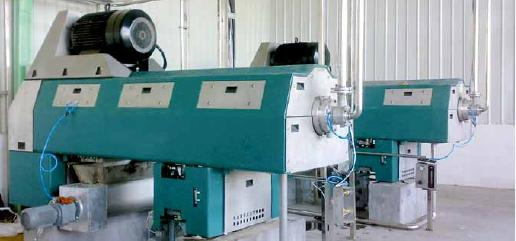
\includegraphics[width=0.8\linewidth]{WestfaliaDouble.jpeg}} 
\caption{ Два декантера <<Westfalia Sepparator>> в процессе обезвоживания барды} 
\label{DublDec} 
\end{figure} 

Основные части декантера <<Westfalia Separator>> "--- барабан и расположенный внутри барабана винтовой шнек. 
Барабан декантера вращается со скоростью в несколько тысяч оборотов в минуту, шнек барды вращается с дифференциальной скоростью, немного большей скорости вращения барабана. 
Исходная барда, поступая внутрь барабана, попадает в поле центробежных сил. 
При этом происходит разделение барды на две фазы: тяжёлую -- твёрдые частицы, которые отбрасываются к стенкам барабана, и лёгкую "--- осветленную тонкую барду, которая выделяется в центральной части барабана ближе к оси вращения. 
Выделенные твёрдые частицы транспортируются винтовым шнеком к конической части барабана (зоне сушки), где происходят их обезвоживание и выгрузка. 
Отвод тонкой барды из декантера осуществляется самотеком или при помощи напорного диска, и далее она поступает на выпарную станцию. 
Степень обезвоживания концентрата барды после сепарации составляет порядка 30\% по сухому веществу. В зависимости от количества исходной барды на стадии обезвоживания могут быть использованы декантеры различной производительности. 
Отечественными учеными Ламм Э.Л., Волчек A.M. и др \cite{Patent_2128688} предложен способ сушки суспензии послеспиртовой барды с получением кормопродукта, включающий анаэробную ферментацию путем последовательного воздействия на компоненты барды комплекса ферментов и кислотообразующих бактерий с получением культуральной жидкости и осадка белкового кормопродукта. 
Существенными недостатками предложенного способа являются: высокая стоимость осуществления из-за сложности технологического процесса; низкая производительность из-за длительности процесса; взрывоопасность; применение сложного и энергоемкого сушильного оборудования. 
Наиболее рациональным и экономически выгодным способом утилизации послеспиртовой зерновой барды является поточная линия для производства сухого белково-витаминного продукта \cite{Patent_2217490}, включающая магистрали для подвода послеспиртовой барды и отвода твердых и жидких продуктов её переработки, и связанные между собой средствами межоперационной передачи, промежуточную емкость, устройство для обезвоживания, выполненное в виде вакуумного фильтра со сходящим полотном и системой непрерывной регенерации ткани, устройство подвода-отвода горячего сухого воздуха, выполненное с возможностью взаимодействия воздуха с твердыми продуктами, вентиляционной камерой и одним циклоном, сушилку, испаритель и барометрический конденсатор с магистралью подвода воды, при этом испаритель и барометрический конденсатор расположены на магистрали подвода вакуума между вакуумным фильтром и его вакуумным насосом, магистраль отвода жидких продуктов переработки связана с испарителем и выполнена в виде затвора, включающего промежуточную емкость для жидких продуктов переработки, устройство для концентрирования фильтрата "--- сепаратор, расположенное на выходе магистрали для отвода жидких продуктов переработки, смеситель, расположенный перед гранулятором и связанный с сепаратором, гранулятор, сборник готовой продукции и устройство для упаковки. 
На сегодняшний день данная линия производства белково-витаминного продукта является одной из немногих, которые позволяют получить наиболее качественный и естественный готовый сухой продукт, с сравнительно низкими капитальными и эксплутационными затратами. 
Однако и ей присущи недостатки: в линии используется роторно-барабанная сушилка, а так как по своему составу барда является высоковлажным и полидисперсным материалам, то при сушке барды в ней наблюдается агрегатирование, комкование, налипание частиц на стенки сушильной камеры, а вследствие этого неоднородность высушивания и возможно обугливание мелких частиц продукта и инкрустация поверхности нагрева частичками барды; высокая энергоемкость процесса из-за использования предварительной сушки дробины перед сушилкой и большого количества вентиляторов; высокая степень уноса частиц продукта, а вследствие этого использование в линии дополнительных циклонов; неэффективное применение сепаратора для концентрирования фильтрата; линия не предусматривает более полное использование компонентов послеспиртовой барды и очистку жидкого отхода, так как не указывается дальнейшее предназначение сепарированного фильтрата. 
В настоящее время в нашей стране машиностроительная промышленность только с недавнего времени начала разрабатывать и внедрять в производство сушильные аппараты для сушки послеспиртовой барды. 
Так, ОАО <<Нежинский механиический завод>> выпускает контактные роторно-дисковые сушилки типа СКМ, (рис.~\ref{CKM} ) 
Корпус представляет собой стальной цилиндр, имеюший паровую рубашку, загрузочный и разгрузочный люк с шибером. 

\begin{figure} 
\centering 
\begin{footnotesize} 
\def\svgwidth{0.95\linewidth} 
\input{figures/DDGS.pdf_tex} 
\end{footnotesize} 
\caption{Сушилка СКМ Нежинского механического завода} 
\label{CKM} 
\end{figure} 

Последний предназначен для регулировки уровня продукта в сушилке. 
Для полного опорожнения сушилки от барды имеется окно. 
Вал представляет собой трубу с расположенными на нём полыми дисками. 
На дисках закреплены лопатки для перемешивания барды и перемещения её к разгрузочному люку. Между дисками устанавливаются скребки для предотвращения застревания продукта и его рыхления. 
Сушка предварительно сгущенной барды происходит за счёт соприкосновения барды с нагреваемыми паром поверхностями дисков, корпуса и вала. 
Кроме того, барда, продвигаясь в осевом направлении, дополнительно сушится встречным потоком воздуха. 
В целях полного использования греющих поверхностей сушилка должна заполняться высушиваемым продуктом на 2/3 объёма корпуса, что контролируется через смотровые окна на боковой крышке. 
Скорость продвижения материала в сушилке можно регулировать изменением положения лопаток во встречных направлениях.
 Аналогичные контактные сушилки марки TST выпускает норвежская фирма <<Stord Internaional>>, а марки PGI-300B -- Цзилинский завод сушильных агрегатов (Китай). 
Конструктивно похожие контактные сушилки шнекового типа марки 133.4 и 133.7 производит ОАО <<Уралхиммаш>> \cite{Korman_2003_7_Journal}. 
Однако процесс сушки послеспиртовой барды в данных аппаратах сопровождается с определенными сложностями. 
Так как при снижении влажности в барде проявляются хорошо выраженные адгезионные и когезионные свойства, барда приобретает студенистую консистенцию, все более густую и при перемешивании наблюдается окомкование (указанные факторы затрудняют процесс обезвоживания), а также данные установки обладают высокой материалоемкостью и энергоемкостью (потребление пара, кг на кг испаренной влаги "--- 1,47). 
Подводя итог вышесказанному, можно сделать вывод, что на данный момент в нашей стране, Европе, США и других странах существует проблема в утилизации послеспиртовой зерновой барде, в несовершенстве технологий и технологического оборудования для осуществления процесса сушки барды. 
Проведя литературный обзор и патентный поиск, выяснилось, что сушку барды в России, Европе, США и ряде других стран проводят преимущественно в барабанных, ленточных, слоевых и ротационных сушилках, которые при высоком потреблении энергии на сушку, не обеспечивают требуемой производительности и качества готового продукта \cite{Antipov_2005_2_Journal,Zhuravlev_2004}. 
Поэтому необходимо совершенствование процесса сушки послеспиртовой барды и оборудования для его осуществления. 
В результате проведения аналитического исследования выявилось, что, так как барда является полидисперсным материалом (неоднородным по составу), то при сушке барды наблюдается комкование, неоднородность высушивания, налипание частиц на стенки сушилки, обугливание мелких частиц продукта и инкрустация поверхности нагрева частичками барды. 
Анализ выявленных особенностей показал целесообразность использования такого вида сушки, при котором каждая частица барды получала бы необходимое количество энергии для фазового превращения содержащейся в ней влаги без образования крупных соединений частиц.

\section{Барда как объект производства}

Химический состав исходного сырья для производства спирта, состав барды из крахмалсодержащего сырья и фракционный состав белка барды представлены в~\cref{tab:grain_chem,tab:stillage_sostav,tab:fraction_sostav}~\cite{Zueva.Fraction.2013}.

\LTXtable{\textwidth}{tabs/grain_chem_sostav}

\LTXtable{\textwidth}{tabs/stillage_sostav}

\LTXtable{\textwidth}{tabs/fraction_sostav}

Сравнительный анализ \cite{Kim.Composition.2008} состава DDGS, фильтрата барды и сухой барды приведен в~\cref{tab:ddgs_stillage_thinstillage}.
Сухая барда и исходная барда богаты глюканом, ксиланом и арабинаном, источниками сбраживаемых сахаров при производстве спирта.
Общее содержание сахаров (глюкан и ксилан) сухой барды и исходной барды 29,4\% и 33,4\% соответственно, в пересчете на сухое вещество.
Сырой протеин составляет 25\% к сухому веществу сухой барды.
Сырой жир составляет 11,6\%
 
\LTXtable{\textwidth}{tabs/sravnenie_product_for_ddgs}

Cпиртовая дробина является ценным продуктом, содержащим незаменимые аминокислоты и имеющая высокую питательную ценность.~\cite[с.~158]{Oleinikov.Svoystva.2010}.
Химический состав различных, сходных по показателям с бардой, продуктов приведены в \cref{tab:chem_sostav_feed_products}, аминокислотный состав "--- в~\cref{tab:aminoacid_sostav_cake_stillage}.%~\cite{Oleinikov.Svoystva.2010}

\LTXtable{\textwidth}{tabs/sravnenie_analiz_barda}

%\LTXtable{\textwidth}{tabs/drobina}

\LTXtable{\textwidth}{tabs/aminoacid_sravnenie}

В~\cite{Liu.Chemical.2011} приведен обзор многочисленных зарубежных источников по анализу состава барды.
Данные сведены в таблицу~\ref{tab:DDGS_analiz}. Минеральный состав приведен в \cref{tab:DDGS_mineral}.

\LTXtable{\textwidth}{tabs/DDGS_analiz}

\LTXtable{\textwidth}{tabs/DDGS_mineral}

Образцы DDGS по~\cite[p.~594]{Rosentrater.Some.2006} имели следующие теплофизические показатели: среднее содержание влаги \(14,7\)\%, активность воды \(0,55\), теплопроводность \(0,07\) \(\text{Вт}/\text{м}\celcius\), сопротивление \(14,0\) \(\text{м}\celcius/\text{Вт}\), коэффициент диффузии \(0,13\) \(\text{мм}^2/\text{с}\), объемная плотность \(483,3\) \(\text{кг}/\text{м}^3\), угол естественного откоса \(31,5^\text{o}\).
Таким образом, свойства барды аналогичны другим сухим кормовым ингредиентам, таких как кукурузный глютен, корма и другим ингредиенты на основе кукурузы.
Теплофизические свойства спиртовой барды на ряде предприятий по~\cite{Rosentrater.Some.2006} приведены в~\cref{tab:stillage_physical}.

\LTXtable{\textwidth}{tabs/stillage_physical}



\section{Теоретические основы выпаривания при утилизации спиртовой барды}

Модель для двухфазного пузырька при барботажном выпаривании задаются уравнениями непрерывности \cite{Campos.Heat.2000} в сферических координатах:
\begin{gather}
\frac{\partial \rho}{\partial t} + \frac{1}{r^{2}}\frac{\partial }{\partial r} (r^{2} \rho v)= 0\label{eq:math_continuity} \\
\frac{\partial}{\partial t}(H \rho)+ \frac{1}{r^{2}} \frac{\partial}{\partial r} \left(r^{2} \rho H v \right)+ \frac{1}{{r}^{2}}\frac{\partial }{\partial r}\left({r}^{2}q\right)=0\label{eq:math_energy} \\
\frac{\partial}{\partial t}(\rho   Y_{i})+ \frac{1}{r^{2}} \frac{\partial}{\partial r} \left[r^{2}  \rho   Y_{i}  \left(v  + W_{i} \right)\right] = 0\label{eq:math_species}
\end{gather}
где \(\rho\)~"--- плотность, \(кг/м^3\); 
\(t\)~"--- время, \(с\);
\(r\)~"--- радиальная координата, \(м\);
\(v\)~"--- радиальная скорость, \(м/c\);
\(H\)~"--- удельная энтальпия, \(кДж/кг\);
\(q\)~"--- тепловая диффузия, \(м^{2}/с\);
\(t\)~"--- массовая доля компонента;
\(W\)~"--- радиальная диффузия, \(м^{2}/c\).

Энтальпия, тепловая  и радиальная диффузия:
\begin{gather}
 H\left(T\right)=\sum _{i=1}^{2}Y_{i}{H}_{i}^{0}\left(T\right)\\
 q=-\lambda \frac{\partial T}{\partial r}+\sum _{i=1}^{2}\rho {H}_{i}^{0}{Y}_{i}{W}_{i}\\
 {W}_{i}=-\frac{{D}_{i}}{{Y}_{i}}\frac{\partial {Y}_{i}}{\partial r} 
\end{gather} 
где \(T\)~"--- температура, \(К\);
\(\lambda\)~"--- коэффициент температуропроводности, \(м^{2}/с\).

Граничные условия на поверхности пузырька для \cref{eq:math_continuity,eq:math_energy,eq:math_species} задаются массовым и энергетическим балансами, которые  получены
из  уравнений непрерывности и выражаются:
 \begin{gather} 
  -\frac{\stackrel{.}{m}}{4\pi {R}^{2}}={\rho }_{S}\left({v}_{S}-\frac{dR}{dt}\right) , \, r=R\left(t\right)\label{eq:math_boundary1} \notag\\
  \left.{\rho }_{S}{D}_{S}{\frac{\partial {Y}_{1}}{\partial r}}\right\vert_{r=R\left(t\right)}=\frac{\stackrel{.}{m}}{4\pi {R}^{2}}\left(1-{Y_1}_{S}\right), \, r=R\left(t\right)\label{eq:math_boundary2}\\
 \left.-\lambda {\frac{\partial T}{\partial r}}\right\vert_{r=R\left(t\right)}=\frac{\stackrel{.}{m}}{4\pi {R}^{2}}{L}_{1}\left({T}_{S}\right)+h\left({T}_{S}-{T}_{L}\right), \, r=R\left(t\right)\label{eq:math_boundary3}\notag
\end{gather} 
где \(\stackrel{.}{m}\)~"--- скорость испарения пузырька, \(К/с\).

Математическая модель процесса барботажного выпаривания, основанная на балансовых уравнения процесса \cite{Reypnazarova.Mathematical.2008} для элементарной зоны барботажного аппарата характеризуется системой уравнений:
\begin{gather}
\frac{d{a}_{i}}{d\tau }=\frac{3}{Vp{K}_{t}}\left({G}_{0}{c}_{1-1}{t}_{i-1}-\frac{{a}_{0}}{{a}_{i}}\right){G}_{1_0}{c}_{i}{t}_{i}- \left(\frac{{a}_{0}}{{a}_{i}-1}-\frac{{a}_{0}}{{a}_{i}}\right){G}_{1_0}I+\notag\\
+\left(\frac{1}{{a}_{i}-2}-\frac{1}{{a}_{i}-1}\right){G}_{0}{a}_{0}{I}_{i}+ KV\left({t}_{2i-2}-{t}_{i-1}\right)\notag\\
 {t}_{i}=\left({G}_{0}+{K}_{i}{c}_{i}\right) \\
 I=\left({I}_{0}+{K}_{i}\left({t}_{2}-{t}_{2_0}\right)\right) \notag\\
 {c}_{1}=\left({c}_{1_0}+K{c}_{1}\left({t}_{1}-{t}_{10}\right)\right) \notag
\end{gather}
где \(G\)~"--- расход теплоты, \(\text{кг}/\text{с}\); \(c\)~"--- теплоемкость, \(\text{кДж}/\text{кгК} \); \(t\)~"--- температура, \(\celcius\);
\(I\)~"--- энтальпия преобразования, \(\text{кДж}/\text{кг}\); \(K\)~"--- коэффициент теплопередачи; \(a\)~"--- элементарная ячейка; \(V\)~"--- объем,
\(\text{м}^{3}\); \(p\)~"--- давление, Па; индексы: \(0\)~"--- начальное состояние; \(1\)~"--- жидкость; \(2\)~"--- газ.

Модель роста парового пузырька в предельно перегретой жидкости~\cite{Aktershev.Rost.2005} сформулирована на основе схемы температурно-однородного равновесного парового пузырька, в которой учитывается изменение давления и плотности пара в пузырьке.

Уравнение динамики парового пузырька:
\begin{equation}
\frac{1}{R}\frac{d}{dt}\left({u}_{1}{R}^{2}\right)=\frac{{p}_{1}-{p}_{0}}{{\rho }_{1}}+\frac{{u}_{1}^{2}}{2} 
\end{equation}
где \(\rho_{1}(t)\)~"---давление в жидкости на межфазной поверхности, \(p_{0}\)~"--- давление
вдали от пузырька.

Граничные условия:
\begin{gather}
{\rho }_{1}\left(\frac{dR}{dt}-{u}_{1}\right)={\rho }_{v}\left(\frac{dR}{dt}-{u}_{2}\right)=j \notag \\
{p}_{1}+\frac{{j}^{2}}{{\rho }_{1}}={p}_{v}+\frac{{j}^{2}}{{\rho }_{\nu }}-\frac{2\sigma }{R}-\frac{4\mu {u}_{1}}{R}\\
 {\lambda }_{v}\frac{\partial {T}_{\nu }}{\partial r}={\lambda }_{1}\frac{\partial {T}_{1}}{\partial r}-jL \notag
\end{gather}
где \({u}_{1}, {u}_{2}\)~"--- соответственно скорости жидкости и пара на межфазной поверхности, \(j\)~"--- плотность потока массы вследствие фазового превращения, \(L\)~"--- теплота фазового перехода.

Уравнение теплопереноса в жидкости:
\begin{equation}
 r\frac{d}{dt}\left(\frac{\Phi }{r}\right)={a}_{T}\frac{{\partial }^{2}\Phi }{\partial {r}^{2}} 
\end{equation}
где \( \Phi\left(r,t\right)=r\left(t\right)\left({T}_{1}-{T}_{0}-\Delta T\right) \).

Начальное и граничные условия:
\begin{equation}
\Phi \left(r, 0\right)=0,~\frac{\partial \Phi \left(\infty, t\right)}{\partial r}=0,~\varphi \left(R,t\right)=R\left(t\right)\left({T}_{\nu }\left(t\right)-{T}_{0}-\Delta T\right) 
\end{equation}

Модель тепло-- массопереноса между пузырьками и жидкостью при барботажном выпаривании~\cite{Guy.Heat.1992} сформулирована на основе уравнения кондукции:
\begin{equation}
 \frac{\partial T}{\partial t}={\nabla }^{2}T 
\end{equation}
где \( t={4t\alpha}/{{d}_{E}^{2}}={Fo}_{t}~\text{"--- число Фурье},~T=\left({T-{T}_{G}}\right/\left({{T}_{L}-T_{G}}\right),~\nabla ={{d}_{E}}/{2} \); \(T\)~"--- температура,~\(\celcius\);
\(t\)~"--- время, c; \(d_{E}\)~"--- эквивалентный диаметр пузырька, м; \(\alpha\)~"--- температуропроводность, \(\text{м}^{2}/\text{с}\); индексы: \(L\)~"--- жидкость, \(G\)~"--- газ.

Начальные и граничные условия:
\begin{equation}
 t=0,~T=0;\; 
  \xi =0,~\frac{\partial T}{\partial \xi }=0;\; 
   \xi =\frac{1}{2},~T=1;\;
    \eta =0,~\frac{\partial T}{\partial \eta }=0;\;
     \eta =\frac{\pi }{2},~\frac{\partial T}{\partial \eta }=0 
\end{equation}

Эффективность массопереноса \({E}_{t}\) в безразмерном виде:
\begin{equation}
 {E}_{t}=\frac{{\iiint }_{\nu }TJ d\xi d\eta  d\varphi }{{\iiint }_{\nu }J\partial \xi d\eta d\varphi } 
\end{equation}
где \(J\)~"--- Якобиан; \(\eta,~\xi,~\varphi\)~"--- эллиптические координаты.

Модель нестационарного процесса в выпарном аппарате с выносной камерой \cite{Ponomarenko.Mathematical.1977} задается уравнением изменения коэффициента теплопереноса от
теплового потока:
\begin{equation}
 \left\{\begin{array}{c}\dfrac{\partial {t}_{1}}{\partial \stackrel{-}{x}}+{a}_{1}{\partial {t}_{1}}/{\partial \tau }={a}_{2}\left({t}_{2}-{t}_{1}\right)+{a}_{3}{G}_{1}\\ {b}_{0}\dfrac{\partial {t}_{2}}{\partial \tau }={b}_{1}\left({t}_{3}-{t}_{2}\right)-{b}_{2}\left({t}_{2}-{t}_{1}\right)-{b}_{3}{G}_{1}\end{array}\right. \end{equation}
где \(a\)~"--- функция температуры \(t\) и массового расхода выпариваемой жидкости \(G\); \({a}_{1}=\dfrac{{m}_{1}}{{G}_{1}}\); \({a}_{2}=\dfrac{{a}_{21}{t}_{1}}{{c}_{1}{G}_{1}} \); \({a}_{3}=\dfrac{{f}_{1}}{{c}_{1}{G}_{1}{\left({t}_{2}-{t}_{1} \right)}_{0}} {\left(\dfrac{\partial {a}_{21}}{\partial {G}_{1}}\right)}_{0}-\dfrac{1}{{G}_{1}}{\left(\dfrac{\partial {t}_{1}}{\partial \stackrel{~}{x}}\right)}_{0} \); \({b}_{0}={c}_{2}{m}_{2}\); \( {b}_{1}={a}_{22}{f}_{3} \); \( {b}_{2}={a}_{21}{f}_{1} \); \( {b}_{3}={f}_{3}{\left({t}_{2}-{t}_{1}\right)}_{0}{\left(\dfrac{\partial {a}_{21}}{\partial {G}_{1}}\right)}_{0} \); \( \stackrel{-}{x}=\dfrac{\partial x}{l} \); \( \stackrel{~}{x}=\dfrac{x}{l} \); \(m\)~"--- масса; \(c\)~"---
теплоемкость; \(t\)~"--- температура; \(\tau\)~"--- время; \(x\)~"--- координата; \(l\)~"--- длина труб аппарата; \(f\)~"--- теплообменная поверхность;
индексы: \(1\)~"--- жидкость; \(2\)~"--- стенка; \(3\)~"---греющий пар.
 
Граничные условия:
\begin{equation}
 {t}_{1}\left(x, 0\right)={t}_{3}\left(x, 0\right);\;  {t}_{1}\left(0, \tau \right)={t}_{10}\left(\tau \right);\;  {t}_{3}\left(0, \tau \right)={t}_{30}\left(\tau \right)  
\end{equation}

Модель неравновесного испарения капель~\cite{Dushin.Mathematical.2008} для многокомпонентной  смеси в представлена виде системы уравнений:
\begin{gather}
\frac{\partial\hat{\rho}}{\partial t}+\frac{1}{x^{k}}\frac{\partial\hat{\rho}vx^{k}}{\partial x}=0, \\
\frac{\partial\hat{\rho}\mathrm{Y}_{i}}{\partial t}+\frac{1}{x^{k}}\frac{\partial\hat{\rho}\mathrm{Y}_{i}vx^{k}}{\partial x}=\frac{1}{x^{k}}\frac{\partial}{\partial x}x^{k}\hat{\rho}D_i\frac{\partial \mathrm{Y}_{i}}{\partial x},\; i=1, \ldots, N, \notag \\
\frac{\partial\hat{\rho}\hat{h}}{\partial t}+\frac{1}{x^{k}}\frac{\partial\hat{\rho}v\hat{h}x^{k}}{\partial x}=\frac{1}{x^{k}}\frac{\partial}{\partial x}x^{k}\lambda\frac{\partial T}{\partial x},
\end{gather}
где \(v\)~"--- скорость; \(x\)~"--- поверхность перехода; \(\mathrm{Y}_{i}\)~"--- массовая концентрация \(i\)--го компонента; \(D_{i}\)~"--- коэффициент
диффузии; \(\lambda\)~"--- теплопроводность; \(T\)~"--- температура; \(k=0, 1\) и \(2\)~"--- соответствуют случаям плоской, цилиндрической и сферической симметрии, соответственно; \(\displaystyle 1/\hat{\rho}=\sum_{i=1}^{N}\mathrm{Y}_{i}/\rho_{i}+L\Delta V_{x}\)~"--- удельный объем и \(\displaystyle \hat{h}=\sum_{i=1}^{N}h_{i}\mathrm{Y}_{i}+L\Delta h_{x}\)~"--- удельная энтальпия
жидкости в смеси; \(L\Delta V_{x}\)~"--- удельный объем и \(L\Delta h_{x}\)~"--- удельная энтальпия растворителя.

Граничные условия для \(x=x_{W}\):
\begin{gather}
\left(\rho v\right)_{g}=\left(\rho v\right)_{l}=\dot{m}, \notag \\ 
\left(\rho v\mathrm{Y}_{j}\right)_{g}-\left(\rho D_{j}\frac{\partial \mathrm{Y}_{i}}{\partial x}\right)_{g}=\left(\rho v\mathrm{Y}_{i}\right)_{l}-\left(\rho D_{i}\frac{\partial \mathrm{Y}_{i}}{\partial x}\right)_{l}=\dot{m}_{i}, \\
\sum_{i=1}^{N}h_{Li}\dot{m}_{i}=\left(\lambda\frac{\partial T}{\partial x}\right)_{g}+\left(\lambda\frac{\partial T}{\partial x}\right)_{l}+\dot{m}L\Delta h_{x}, \notag
\end{gather}
где \(h_{Li}\)~"--- удельная энтальпия фазового перехода; индексы: \(g\)~"--- газовая фаза; \(l\)~"--- жидкая фаза.
 Дополнительным условием служит уравнение Герца---Кнудсена:
\begin{equation}
p_{i}=p_{e}X_{j}=p_{i}^{*}\left(T_{W}\right)-\displaystyle \frac{1}{\delta_{i}}\sqrt{\frac{2\pi RT}{m_{i}}}\dot{m}_{i}
\end{equation} 
где \(X_{i}\)~"--- молярная концентрация; \(p_{i}\)~"--- парциальное давление; \(\delta_{i}\)~"--- коэффициент аккомодации; \(p_{i}^{*}(T_{W})\)~"---  равновесное давление паров \(i\)--го компонента при температуре \(T_{W}\).


\section{Применение выпарных аппаратов при выпаривании фильтрата барды}

\subsection{Выпарные аппараты общего назначения}

% Промышленный выпарной аппарат \cite{Shinsuke.Industrial.2005} представлен на \cref{fig:industial_evaporation_app}.
% 
% \begin{wrapfigure}{R}{0.5\textwidth}
% \centering
% \includegraphics[width=0.48\textwidth]{figures/temp/shinsuke.jpg}
% \caption{Промышленный выпарной аппарат: 1 "--- патрубок исходной жидкости, 2 перфорированная пластина, 3 "--- зона подачи исходной жидкости, 4 "--- направляющие, 5 "--- зона испарения, 6 "--- патрубок удаления выпаренного раствора, 7 "--- патрубок удаления жидкости, 8 "--- насос удаления жидкости, 9 "--- патрубок
% подачи теплового агента, 10 "--- боковая стенка корпуса зоны испарения, 11 "--- конусная стенка зоны испарения, 20 "--- жидкость на выходе.}\label{fig:industial_evaporation_app}
% \end{wrapfigure}

% Выпарной аппарат с восходящей и нисходящей пленками \cite{Petrov.Vyparnoy.2002} изображен на~\cref{fig:evaporation_app_up_down} 
% 
% \begin{wrapfigure}{R}{0.5\textwidth}
% \centering
% \includegraphics[width=0.48\textwidth]{figures/temp/petrov.jpg}
% \caption{Выпарной аппарат с восходящей и нисходящей пленками}\label{fig:evaporation_app_up_down}
% \end{wrapfigure}
\begin{wrapfigure}{r}{0.5\textwidth}
\centering
\includegraphics[width=0.48\textwidth]{figures/temp/ostrikov.jpg}
\caption[Вакуум-выпарной аппарат]{Вакуум-выпарной аппарат: 1~"--- корпус, 2~"--- верхняя крышка, 5, 6~"--- патрубки для удаления испаряемых паров, 7~"--- рубашка, 8~"--- патрубок для подвода горячего теплоносителя, 9~"--- патрубок для отвода отработанного теплоносителя, 3~"--- комбинированная мешалка, скребки: 20, 22~"--- серповидные, 21~"--- лемехообразные, 26~"--- нижняя камера аппарата, 27~"--- верхняя камера аппарата, 12, 13~"--- трубопровод, 25~"--- сепаратор, 4, 19~"--- подшипниковые опоры, 23~"--- вал, 11~"--- форсунки, 14~"--- насос, 28~"--- торообразная камера, 15~"--- распылительные форсунки, 17~"--- торцевые уплотнения, 16~"--- электродвигатель, 29~"--- муфта, 6~"--- патрубок, 18~"--- полое кольцо, 10~"--- кольцевой желоб, 24~"--- патрубок удаления продукта.}\label{fig:evaporation_app_ostrikov}
\end{wrapfigure}
Вакуум-выпарной аппарат \cite{Ostrikov.Vakuum.2011} (рисунок~\ref{fig:evaporation_app_ostrikov}) работает следующим образом: включается привод вакуум-насоса (не показан), соединенного с патрубками 5 и 6, и в камерах 26 и 27 создается заданная величина разрежения.
Одновременно в рубашку 7 через патрубок 8 подается горячий теплоноситель с заданной температурой, нагревая внутреннюю боковую стенку в камерах 26 и 27.
Далее включается регулируемый привод (не показан), который приводит во вращательное движение мешалку 3.
Также включается электродвигатель 16, приводящий во вращательное движение форсунки 15.
Затем подогретое до заданной температуры исходное фруктовое или овощное пюре нагнетательным насосом (не показан) подается через трубу 12 во вращающиеся форсунки 11.
За счет конструкции распылительных форсунок 11 продукт (фруктовое или овощное пюре) распыливается в виде мелкодиспергированных капель, имеющих
колоколообразную форму.
Затем капли фруктового или овощного пюре оседали на поверхности конусной части корпуса 1, формируя пленку продукта, которая с помощью серповидных скребков 20, закрепленных на мешалке 3, перемещалась к выгрузочному отверстию, соединенному с трубопроводом 13.
Серповидные скребки 20 не только перемещают продукт к трубопроводу 13, но и интенсивно его перемешивают, обеспечивая при этом дополнительное выпаривание влаги из продукта, т.к. внутренняя поверхность камер 26 и 27 обогревается с помощью рубашки 7. 
При этом за счет дополнительного нагрева продукта от поверхности конусной части корпуса 1 происходит дополнительное выпаривание влаги из продукта.
Испаряемые из пюре водяные пары в нижней камере 26 удаляются через патрубок 6, соединенный с вакуум-насосом.
Далее продукт по трубопроводу 13 нагнетается насосом 14 в кольцевую торообразную камеру 28, на боковой поверхности которой с равным шагом радиально расположены распылительные форсунки 15.
Вращающиеся при помощи электродвигателя 16 и муфты 29 распылительные форсунки 15 распыливают продукт (фруктовое или овощное пюре) в виде мелкодиспергированных капель.
Форма и конструкции форсунок 15 обеспечивали равномерный режим распыливания по всему объему камеры 27. 
Затем капли фруктового или овощного пюре оседали на поверхности цилиндрической части корпуса 1, образуя пленку продукта, постепенно стекающую вниз под действием сил тяжести.
При контакте капель пюре с обогреваемой поверхностью происходил нагрев пленки пюре, стекающей вниз, и испарение влаги из пюре за счет термостатируемой внутренней стенки вакуум-выпарного аппарата.
Лемехообразные скребки 21, установленные на мешалке 3, счищают и постепенно плавно перемещают вниз слой овощного или фруктового пюре.
Серповидные скребки 22, установленные на мешалке 3, предназначены для удаления продукта с верхней поверхности сепаратора 25 и нанесения продукта тонким равномерным слоем по внутренней цилиндрической поверхности камеры 26.
Испаряемые из пюре водяные пары в верхней камере 27 удаляются через патрубки 5, соединенные с вакуум-насосом.
Концентрированный продукт (сгущенная суспензия), стекая по вертикальной
боковой стенке нижней камеры 26, попадает в кольцевой желоб 10 и выводится из аппарата через патрубок 24 для дальнейшей переработки.
\begin{figure}[htb]
\centering
\includegraphics[width=0.52\textwidth]{figures/temp/voynov.jpg}
\caption[Пленочный выпарной аппарат]{Пленочный выпарной аппарат: 1~"--- вертикальный цилиндрический корпус, 2~"--- крышка, 3~"--- днище, штуцера: 4,5~"---  для ввода и вывода раствора, 6~"--- вывода конденсата вторичного пара, 7, 8~"--- подвода и отвода теплоносителя, 9, 10~"--- подвода и отвода хладагента, 11~"--- вспомогательный, 12, 13~"--- камеры для ввода раствора и вывода концентрированного раствора, 14~"--- греющая камера, трубопроводы: 15, 16~"--- для подвода и отвода хладагента, 17~"--- отвода конденсата вторичного пара, 18~"--- цилиндрические трубы, 19~"--- кольцевая спираль, 20~"--- внутренние трубы, 21~"--- витки, 22~"--- патрубок для отвода конденсата вторичного пара, 23~"--- шайбы, 24~"--- ограничительные ребра, 25~"--- профилированные пластины, 26~"--- боковая кромка, 27~"--- каналы для прохода парожидкостной смеси, 28~"--- втулка для распределения жидкости, 29~"--- заглушка, 30~"--- ребра для обеспечения зазора и крепления, 31~"--- продольные канавки для отвода уловленных капель раствора, 32~"--- лист из пористого материала, 33~"--- воронки, 34~"--- пластинки, 35~"--- зазор для прохода конденсата вторичного пара.}\label{fig:evaporation_app_voynov}
\end{figure}

Пленочный выпарной аппарат \cite{Voynov.Plenochniy.2006} представлен на~\cref{fig:evaporation_app_voynov}.
Раствор через штуцер 4 поступает в камеру 12, распределяется на верхней горизонтальной перегородке, а затем поступает в кольцевые зазоры, образованные внутренней поверхностью цилиндрической трубы 18 и наружной поверхностью втулки, для распределения жидкости 28, выйдя из которых, раствор стекает в виде жидкостной пленки по внутренней поверхности цилиндрических труб, интенсивно перемешиваясь, обтекая витки кольцевой спирали 19.
При этом происходит нагревание раствора через стенку цилиндрических труб теплоносителем, поступающим через штуцер 7 в греющую камеру 14, вследствие чего раствор закипает, образуется отток вторичного пара и капель раствора (парожидкостная смесь) с поверхности пленки.
Парожидкостная смесь проходит по каналам 27, образованным профилированными пластинами 25, приобретает вращательнопоступательное движение, вследствие чего возникает центробежная сила, которая отбрасывает часть капель на поверхность пластин, которые затем по канавкам 31 стекают в камеру концентрированного раствора 13.
В случае наличия на поверхности пластин листа 32, выполненного из перфорированного материала, капли раствора по каналам, образованным порами пористого материала, также стекают вниз в камеру 13.
Другая часть капель в месте с потоком вторичного пара, выйдя из каналов 27, вследствие вращательного движения приобретает форму жидкостного кольца и под действием силы тяжести стекает вниз в камеру 13.
Освободившийся от капель вторичный пар конденсируется на поверхности внутренних труб 20, в полость которых подается охлаждающая вода через штуцер 9 и трубопроводы 15.
Отвод охлаждающей воды осуществля ется через трубу 16, соединенную со штуцером 10.
Образовавшийся конденсат по виткам 21 поступает на поверхность воронок 33 и через зазоры 35 стекает во внутрь витков, а затем в полость патрубков 22, через которые по трубопроводу 17 выводится из аппарата.
Сконцентрированный раствор на выходе из цилиндрических труб поступает в камеру 13, а затем через штуцер 5 выводится из аппарата.

\subsection{Барботажно-выпарные аппараты}
\begin{wrapfigure}{R}{0.52\textwidth}
\centering
\includegraphics[width=0.4\textwidth]{figures/temp/rabiner.jpg}
\caption[Выпарной аппарат для концентрирования растворов путем непосредственного контакта с газообразным теплоносителем]{Выпарной аппарат для концентрирования растворов путем непосредственного контакта с газообразным теплоносителем: 1~"--- вертикальный корпус, 2~"--- крышка, патрубки: 3~"--- подачи исходного раствора, 4~"--- отвода упаренного раствора, 5~"--- отвода парогазовой смеси, 6~"--- барботажные трубы, 7~"--- циркуляционная труба, 8~"--- кольцевой кожух, 9, 10~"--- коаксиальный цилиндр.}\label{fig:evaporation_app_rabiner}
\end{wrapfigure}
Выпарной аппарат (рисунок~\ref{fig:evaporation_app_rabiner}) для концентрирования растворов путем непосредственного контакта с газообразным теплоносителем~\cite{Rabiner.Vypanroy.1979} работает следующим образом: газообразный теплоноситель, например продукты сгорания топлива, по барботажным трубам 6 поступает в кольцевой кожух 8, откуда распределяется в центральную часть кожуха, ограниченную внутренним цилиндром 9, и в объем между циркуляционной трубой 7 и наружным цилиндром 10 кожуха 8.
Исходный раствор по патрубку 3 подается в центральную часть кожуха 8, где он в противотоке взаимодействует с газообразным теплоносителем, выходящим из полости кожуха 8.
Одновременно газообразный теплоноситель в объеме между циркуляционной трубой 7 и кожухом 8, двигаясь в прямотоке с раствором, создает его естественную циркуляцию в аппарате 1.
Упаренный раствор накапливается в нижней части аппарата 1 и непрерывно выводится через патрубок 4.
Парогазовая смесь сепарируется на жалюзийных насадках и непрерывно выводится из аппарата через патрубок 5.

\begin{figure}
\centering
\begin{minipage}{.45\textwidth}
\centering
\includegraphics[width=0.8\textwidth]{figures/temp/kasatkin.jpg}
\caption[Выпарной аппарат погружной горелкой]{Выпарной аппарат погружной горелкой:  1~"--- корпус, 2~"--- горелка, 3~"--- переливная труба, 4~"--- сепаратор.}\label{fig:evaporation_app_kasatkin}
\end{minipage}%
~
\begin{minipage}{.45\textwidth}
\centering
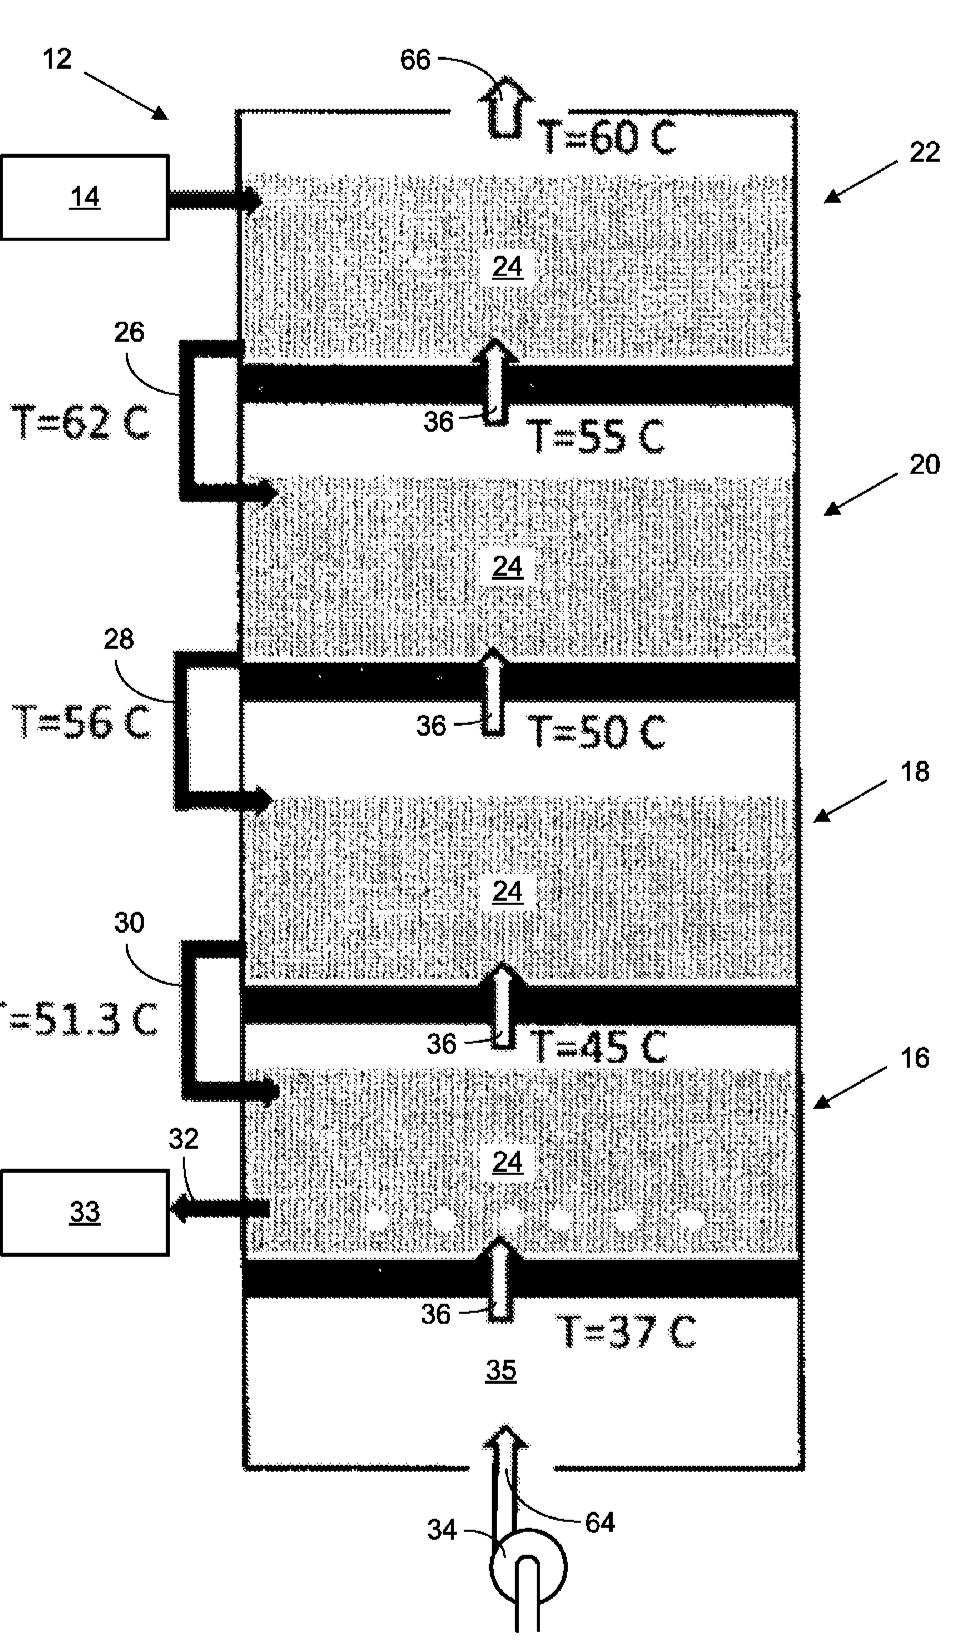
\includegraphics[width=0.5\textwidth]{figures/temp/Govindan.jpg}
\caption[Многокорпусной барботажно-выпарной аппарат]{Многокорпусной барботажно-выпарной аппарат: 12~"--- аппарат, 16, 18, 20, 22~"--- камера испарителя, 24~"--- ванна, 26, 28, 30, 32~"--- трубопровод, 34~"--- вентилятор, 64~"--- воздуховод.}\label{fig:evaporation_app_govindan}
\end{minipage}
\end{figure}


Барботажный выпарной аппарат с погружными горелками~\cite{Kasatkin.Processi.1971} изображен на~\cref{fig:evaporation_app_kasatkin}.
В плоской крышке корпуса 1 аппарата расположена одна горелка 2 или несколько горелок, погруженных под уровень выпариваемого раствора.
Уровень раствора в аппарате поддерживается постоянным с помощью переливной трубы 3.
Упаренный раствор отводится из конического днища аппарата, а выпадающие здесь кристаллы отсасываются посредством эрлифта.
Паро-газовая смесь от водится из пространства над жидкостью через сепаратор 4.
Многокорпусной барботажно-выпарной аппарат \cite{Govindan.Multi.2015} представлен на~\cref{fig:evaporation_app_govindan}.
Жидкость, содержащую растворенные компоненты подают из сборника 14 в камеру 22 испарителя 12, где жидкость образует ванну 24, содержащейся в камере четвертого стадии 22.
Исходную жидкость подают в камеру 22 для увлажнения четвертой стадии при температуре 70\(\celcius\).
Испаренный компонент (например, вода) из исходной жидкости испаряется газом, пузырьки которого подают через ванну 24.
Остатки жидкости подают из камеры 22 по трубопроводу 26 в камеру третьей ступени 20, в которой подают газ.
Остаток исходной жидкости подают в камеру третьей ступени 20 при температуре 62 С
Температура оставшейся жидкости уменьшается от стадии к стадии, в частности, с помощью энергии, используемой для испарения испаряемого компонента из исходной жидкости на каждой стадии.

Аппарат для перегонки улучшенной эффективности~\cite{Lee.Fluid.2007} представлен на~\cref{fig:evaporation_app_lee}.
Цилиндрический корпус 100 выполнен с возможностью контроля уровня воды или других жидкостей 111.
Воду или другие жидкости для дистилляции 112 подают в корпус 100 через впускное отверстие 113.
Сливной патрубок 114 предназначен для периодического удаления солоноватой жидкости конденсатора, который собирается в нижней части корпуса 100.
Паровое пространство 116 сформировано на верхнем конце внутренней корпуса 100, как правило над поверхностью жидкости 111.
Множество спиральных конденсирующих труб 117 расположены кольцеобразно на внешней периферии внутренней части корпуса 100.
Пар из парового пространства 116 поступает в конденсационные трубы 117, как указано стрелками 126 и 130.
Пары идущий по конденсационным трубам 117 вступает в теплообмен с жидкостью и конденсируется, производя дистиллят.
Дистиллят удаляют через коллектор 118 он содержит общее выпускное отверстие 119.
Барботирование газом 121 по трубе 122, имеющей отверстия 123 осуществляют в межтрубное пространство теплообменных труб 117, которые производят пузыри 124.
\begin{figure}[tb]
\centering
\includegraphics[width=0.5\textwidth]{figures/temp/lee.jpg}
\caption[Аппарат для перегонки улучшенной эффективности]{Аппарат для перегонки улучшенной эффективности: Цилиндрический корпус 100, уровень 111 жидкости, жидкости для дистилляции 112, впускное отверстие 113, сливной патрубок 114, паровое пространство 116, спиральные конденсирующие трубы 117, пар 126 и 130, коллектор 118, выпускное отверстие 119, камера конденсация 120, газ 121, труба для барботирования 122, отверстия для барботирования 123, пузыри 124, камера нагрева 127, трубчатая стенка 131, нагревательный элемент 128.}\label{fig:evaporation_app_lee}
\end{figure}
Пузыри поднимаются вверх в кольцевую камеру конденсации 120.
Геометрия камеры нагрева 127 задается трубчатой стенкой 131, окружающей нагревательный элемент 128.
Вода из камеры 120 конденсации проходит в глубь нагревательной камеры 127 через отверстие 133 в нижней ее части.
Нагревательный элемент 128 производит пузырьки пара 132, которые проходят вверх через верхнее отверстие 129 в камере нагрева в паровое пространство 116.
Затем пар поступает в конденсационные трубы, как показано стрелкой 130, и было описано ранее.




\section{Инженерные методы расчета}

\subsection{Вакуум-выпарной аппарат}\label{seq:calculation_vacuum}

Количество выпариваемой воды, \(\text{кг}/\text{ч}\) определяют по уравнению:
\begin{equation}
 W={G}_{\text{н}}\left(1-\frac{{w}_{\text{н}}}{{w}_{\text{к}}}\right), 
\end{equation}
где \({G}\)~"--- производительность по жидкости, \(\text{кг}/\text{ч}\); \(w\)~"--- влажность; индексы: \(\text{н}\)~"--- начальное значение; \(\text{к}\)~"---
конечное значение.

Расход теплоты на выпаривание \(Q\) включает затраты тепла на нагрев \(Q_{\text{нагр}}\), испарение \(Q_{\text{исп}}\), дегидратацию и потери в окружающую
среду (принимаются равными \(10\)\% от \(\left(Q_{\text{нагр}} + Q_{\text{исп}}\right)\)).

Расход тепла на нагрев, \(\text{ккал}/\text{ч}\) находят по уравнению:
\begin{equation}
 {Q}_{\text{нагр}}={G}_{\text{н}}{c}_{\text{н}}\left({t}_{\text{кип}}-{t}_{\text{н}}\right),
\end{equation}
где \(t\)~"--- температура, \(\celcius\); индексы: \(\text{кип}\)~"--- кипение.

Расход тепла на испарение, \(\text{ккал}/\text{ч}\):
\begin{equation}
 {Q}_{\text{исп}}=Wr,
\end{equation}
где \(r\)~"--- теплота парообразования, \(\text{ккал}/\text{кг}\).

Общий расход тепла в аппарате, \(\text{ккал}/\text{ч}\):
\begin{equation}
 Q=\left({Q}_{\text{нагр}}+{Q}_{\text{исп}}\right)\cdot 1,1 
\end{equation}

Расход греющего пара, \(\text{кг}/\text{ч}\):
\begin{equation}
D=\frac{Q}{{r}_{\text{г. п.}}},
\end{equation}
где \({r}_{\text{г. п.}}\)~"--- теплота конденсации греющего пара, \(\text{ккал}/\text{кг}\).

Удельный расход пара, \(\text{кг}/\text{кг}\):
\begin{equation}
 d=\frac{D}{W} 
\end{equation}

Поверхность нагрева, \(\text{м}^{2}\):
\begin{equation}
 F=\frac{Q}{{K}_{\Delta }{t}_{\text{пол}}},
\end{equation}
где \(K\)~"--- коэффициент теплопередачи в теплообменнике, \(\text{ккал}/\left(\text{м}^{2}\text{ч}\celcius\right)\); 
\(\Delta {t}_{\text{пол}}={t}_{\text{г.п.}}-{t}_{\text{кип}} \)~"--- полезная разность температур, \(\celcius\)


\subsection{Барботажный выпарной аппарат}

Теоретическое количество воздуха \(\text{кг}/\text{кг}\), необходимое для сжигания \(1\) \(\text{м}^{3}\) природного газа:
\begin{equation}
 {L}_{0}=9,4\frac{{\rho }_{\text{в}}}{{\rho }_{\text{т}}}, 
\end{equation}
где \(\rho\)~"--- плотность, \(\text{кг}/\text{м}^{3}\); индексы: \(\text{в}\)~"--- воздух; \(\text{т}\)~"--- топливо.

Количество водяных паров, образующихся при сжигании 1 кг газа, \(\text{кг}/\text{кг}\):
\begin{equation}
 {G}_{\text{п}}=\sum \frac{0,09}{12m+n}{C}_{m}{H}_{n} 
\end{equation}

Количество сухих газов, образующихся при сжигании \(1\) кг природного газа, \(\text{кг}/\text{кг}\):
\begin{equation}
 {G}_{\text{с. г.}}=1+\alpha {L}_{0}-{G}_{\text{п}},
\end{equation}
где \(\alpha\)~"--- коэффициент избытка воздуха.

Количество водяных паров в топочных газах, \(\text{кг}/\text{кг}\):
\begin{equation}
 {G}_{\text{п}}^{\prime }=\frac{\alpha {d}_{0}{L}_{0}}{1000}+{G}_{\text{п}},
\end{equation}
где \({d}_{0}\)~"--- влагосодержание сухого воздуха, \(\text{г}/\text{кг}\).

Влагосодержание топочных газов, \(\text{г}/\text{кг}\):
\begin{equation}
 {d}_{вх}=\frac{{G}_{1}\cdot 1000}{{G}_{\text{с. г}}} 
\end{equation}

Расход топочных газов, \(\text{кг}/\text{ч}\):
\begin{equation}
 L=\frac{Q}{{c}_{\text{вх}}{t}_{\text{вх}}-{c}_{\text{вых}}{t}_{\text{вых}}} 
\end{equation}

Расход тепла с отходящими из выпарного аппарата газами, \(\text{ккал}/\text{ч}\):
\begin{equation}
 {Q}_{1}=L{c}_{\text{от. г}}\left({t}_{\text{вых}}-{t}_{0}\right) 
\end{equation}

Суммарный расход тепла, вносимого в выпарной аппарат, \(\text{ккал}/\text{ч}\):
\begin{equation}
 \sum Q=Q+{Q}_{\text{от. г}},
\end{equation}
где \(Q\) определяют из соответствующих уравнений рассмотренных в~\cref{seq:calculation_vacuum}.

Расход топлива, \(\text{м}^{3}/\text{ч}\):
\begin{equation}
 B=\frac{\sum Q}{{Q}_{\text{н}}{\eta }_{т}},
\end{equation}
где \({Q}_{\text{н}}\)~"--- низшая теплота сгорания топлива, \(\text{ккал}/\text{ч}\); \({\eta }_{т}\)~"--- КПД топки.

Удельный расход тепла, \(\text{м}^{3}/\text{ч}\):
\begin{equation}
 q=\frac{B{Q}_{\text{н}}}{W} 
\end{equation}

Влагосодержание газов на выходе из аппарата, \(\text{г}/\text{кг газа}\):
\begin{equation}
 {d}_{\text{вых}}={d}_{\text{вх}}+\frac{W\cdot 1000}{L} 
\end{equation}

Удельный объем газов на входе/выходе, \(\text{м}^{3}/\text{ч}\):
\begin{equation}
{\nu }_{\text{вх(вых)}}^{0}=4,64\cdot {10}^{-6}\left(622+{d}_{вх(вых)}\right)\left(273+{t}_{вх(вых)}\right)
\end{equation}

Объем газов на входе/выходе,  \(\text{м}^{3}/\text{ч}\):
\begin{equation}
 {\nu }_{\text{вх(вых)}}={\nu }_{\text{вх(вых)}}^{0}L 
\end{equation}

Определение <<зеркала>> испарения аппарата, \(\text{м}^{2}\):
\begin{equation}
 F=\frac{{\nu}_{\text{вых}}}{{w}_{2}\cdot 3600},
\end{equation}
где \(w_{2}\)~"--- скорость газов в горизонтальном сечении аппарата.

Определения диаметра барботажных труб:
\begin{equation}
 F=\frac{{\nu}_{\text{вх}}}{{w}_{1}\cdot n \cdot 3600},
\end{equation}
где \(w_{1}\)~"--- скорость в барботажной трубе; \(n\)~"--- число труб.

Тогда диаметр труб, \(\text{м}\):
\begin{equation}
 d=\sqrt{\frac{4F}{\pi }} 
\end{equation}


\section{Технологические схемы переработки спиртовой барды}

Известен способ приготовления кормовой добавки (рисунок~\ref{fig:stillage_bumbar}) на основе послеспиртовой барды и сои~\cite{Bumbar.Sposob.2003}.
Послеспиртовую барду с содержанием СВ\(=\)6--8\% объема центробежным насосом 1 из бардяной ямы 2 перекачивают в чан-сборник барды 3.
\begin{figure}[htb]
\centering
\includegraphics[width=\textwidth]{figures/temp/bumbar.jpg}
\caption[Способ приготовления кормовой добавки на основе послеспиртовой барды и сои]{Способ приготовления кормовой добавки на основе послеспиртовой барды и сои: 1, 9~"--- центробежный насос, 2~"--- бардяная яма, 3~"--- чан-сборник барды, 4, 7~"--- шнековый фильтр-пресс, 5, 8~"--- сборник фильтрата барды, 6, 15, 19~"--- шнековый транспортер, 10~"--- выпарная установка, 11, 16~"--- смеситель, 12~"--- испаритель, 13~"--- сушилка, 14~"--- молотковая дробилка, 17, 18~"--- сборник, 20~"--- гранулятор.}\label{fig:stillage_bumbar}
\end{figure}

Из чана-сборника 3 барду самотеком направляют в шнековый фильтр-пресс 4.
Из фильтр-пресса 4 фильтрат барды до 50\% объема с концентрацией СВ\(=\)2--3\% направляют самотеком в сборник фильтрата барды 5 и в последующем центробежным насосом перекачивают на технологические нужды спиртового производства: на рассортировку помола крахмалосодержащего сырья и для разжижения бражки.
Оставшуюся барду с содержанием СВ\(=\)25--30\% шнековым транспортом 6 направляют на второй фильтр пресс 7. 
Из фильтр--пресса 7 фильтрат барды СВ\(=\)3\% самотеком поступает в сборник фильтрата барды 8 и центробежным насосом 9 направляют в выпарную установку 10.
Барду с содержанием СВ\(=\)35--40\% с фильтр--пресса 7 направляют в смеситель 11, сюда же одновременно подают соевый помол до 40\% к объему барды, мел, соль, конденсат из испарителя 12 и самотеком из выпарной установки 10 бардяной концентрат СВ\(=\)40--50\%.
В рубашку сушилки 13 падают пар под давлением 5--6 атм.
Температура в сушилке поддерживается 130--140\(\celcius\). 
Из роторно--дисковой сушилки кормовая смесь с содержанием СВ\(=\)90--92\% поступает в молотковую дробилку 14, испарившуюся влагу кормовой смеси из сушилки направляют в испаритель 12.
Выходящий из молотковой дробилки 14 помол перемещают шнековым транспортером 15 в смеситель 16, где его смешивают с минеральными добавками и витаминами, поступающими в смеситель 16 из сборников 17 и 18.
Перемешанную кормовую массу подают шнековым транспортером 19 в гранулятор 20.
С гранулятора готовую к скармливанию кормовую добавку затаривают в мешки и направляют на реализацию.

Технологическая линия производства белково-витаминного кормопродукта из послеспиртовой зерновой барды~\cite{Antipov.Technologycal.2005} представлена на~\cref{fig:stillage_antipov}.
\begin{figure}[htb]
\centering
\includegraphics[width=\textwidth]{figures/temp/antipov.jpg}
\caption[Технологическая линия производства белково-витаминного кормопродукта из послеспиртовой зерновой барды]{Технологическая линия производства белково-витаминного кормопродукта из послеспиртовой зерновой барды: 1~"--- промежуточная емкость, 2~"--- устройство для обезвоживания, 3, 8~"--- вентилятор, 4~"--- калорифер, 5~"--- вихревая сушилка, 6~"--- смеситель, 7~"--- циклон, 9~"--- гранулятор, 10~"--- вентиляционная камера, 11~"--- сборник готовой продукции, 12~"--- устройство для упаковки, 13~"--- испаритель, 14~"--- вакуумный насос, 15~"--- барометрический конденсатор, 16~"--- промежуточная емкость, 17~"--- устройство для концентрирования фильтрата.}\label{fig:stillage_antipov}
\end{figure}
Послеспирт\-овая зерновая барда из брагоперегонного аппарата по магистрали подвода послеспиртовой зерновой барды поступает в промежуточную емкость 1, где аккумулируется в необходимом объеме для бесперебойной работы вакуумного фильтра 2 типа БОП со сходящим полотном и системой непрерывной регенерации ткани.
После вакуумного фильтра 2 послеспиртовая барда разделяется на два потока, один из которых включает твердый продукт (дробина), а другой~"--- жидкий (фильтрат).
Дробина выглядит как рыхлая масса с влажностью от 40\% до 60\%. Фильтрат включает в себя 2\dots4\% сухих веществ, часть которых находится во взвешенном состоянии, а часть растворена.
Работу фильтра 2 обеспечивает вакуумный насос 14.
Для получения более глубокого вакуума используют испаритель 13 и барометрический конденсатор 15.
С полотна вакуумного фильтра 2 дробину при помощи средства межоперационной передачи подают в сушилку 5.
После сушилки 5 дробина имеет влажность 15\dots20\% и ее можно подвергать грануляции в устройстве 9.
Из гранулятора 9 продукт попадает в вентиляционную камеру 10, где обдувается горячим сухим воздухом, поступающим из калорифера 4, доводится до содержания влаги 6\dots10\%, после чего он поступает в сборник 11 готовой продукции, упаковывается на устройстве 12, например, в мешки или насыпается россыпью в запирающуюся тару и отвозится на склад или потребителю.
Для увеличения выхода продукта и очистки отработанного воздуха из устройств 5 и 10 последний проходит через воздухоочиститель циклонного типа~"--- циклон 7, в котором отделяются твердые частицы белково-витаминного продукта, поступающие в дальнейшем в гранулятор 9.
В атмосферу выбрасывается практически чистый воздух.

Способ приготовления сухой барды и установка для его осуществления~\cite{Ezhkov.Sposob.2005} изображена на~\cref{fig:stillage_ezhkov}.
Исходную послеспиртовую барду подают в камеру подготовки 6 по тракту загрузки 7.
Одновременно через тракт загрузки 7 в камеру 6 подают и требуемое количество сухого продукта.
Количество подаваемого сухого продукта регулируют в зависимости от состава и консистенции послеспиртовой барды, типа сушильной камеры, вида несущей поверхности и т.п.
\begin{figure}[htb]
\centering
\includegraphics[width=\textwidth]{figures/temp/ezhkov.jpg}
\caption[Способ приготовления сухой барды и установка для его осуществления]{Способ приготовления сухой барды и установка для его осуществления: 1~"--- сушильный аппарат, с входным 2 и выходным 3 участками, 4~"--- раздаточный узел, 5~"--- блок повышения содержания сухих веществ, 6~"--- камера подготовки исходной послеспиртовой барды, 7, 8~"--- тракт загрузки и выгрузки соответственно, 9~"--- накопительный бункер, 10~"--- режущий скребок, 11~"--- рециркуляционная линия, 12~"--- несущая поверхность.}\label{fig:stillage_ezhkov}
\end{figure}
Для широкого спектра использующейся послеспиртовой барды оптимальным значением количества сухого продукта является 40--60\% от массового расхода исходной барды.
Предварительно, перед подачей в камеру подготовки, сухой продукт измельчают до размера частиц не более 1 мм.
Послеспиртовую барду и сухой продукт смешивают в камере 6 до образования однородной смеси, после чего образованную смесь с заданным содержанием сухих веществ в ней выводят из камеры 6 по тракту выгрузки 8.
С помощью подключенного к тракту выгрузки 8 раздаточного узла 4 на несущей поверхности 12 формируют сплошной слой барды не более 2 мм, и сформированная таким образом барда поступает на сушку в сушильный аппарат 1.
Перед операцией формования барды несущую поверхность смачивают веществом, предотвращающим прилипание барды к поверхности, например пищевым растительным маслом.
Т.к. образованная смесь, по существу, на 50\% состоит из частиц сухого продукта, смоченного исходной жидкой послеспиртовой бардой, процесс сушки такой смеси сводится к высушиванию внешней поверхности упомянутых частиц и поэтому значительно интенсифицируется.
После высушивания до требуемой кондиции высушенная барда подается к накопительному бункеру 9, где отделяется от несущей поверхности 12 с помощью режущего скребка 10, и полученный сухой продукт частично возвращается по рециркуляционной линии 11 в камеру подготовки 6, а остальной сухой продукт выводится по технологическому назначению.

Схема технологии получения сухой барды стандарта DDGS из отходов спиртового производства~\cite{CH.Device.2006} приведена на~\cref{fig:stillage_chinese}.
\begin{figure}[htb]
\centering
\includegraphics[width=\textwidth]{figures/temp/chinese.jpg}
\caption[Технология получения DDGS продукта из отходов спиртового производства]{Технология получения DDGS продукта из отходов спиртового производства:
1~"--- сепаратор, 2~"--- выпарная установка, 4~"--- смеситель, 5~"--- сушилка: 5--1~"--- парогенератор, 5--3~"--- первая вихревая сушилка, 5--4, 5--7~"--- циклон, 5--5~"--- генератор горячего воздуха, 5--6~"--- вторая вихревая сушилка, 5--8~"--- вентилятор.}\label{fig:stillage_chinese}
\end{figure}
Барду из цеха подают в сепаратор 1, далее фильтрат направляют в выпарной аппарат 2 и затем в смеситель 4, куда подают твердую фазу после сепаратора 1.
После смешивания продукт подают в сушилку 5, включающую в себя парогенератор 5--1, вихревые сушилки 5--3 и 5--6, циклоны 5--4 и 5--7.
Материал высушивается горячим воздухом от генератора горячего воздуха 5--5 подключенного к обоим сушилкам 5--3 и 5--6. 
Испарившийся из материала пар после циклона 5--4, направляется в выпарной аппарат 2, смешиваясь в соединительном трубопроводе циркуляционным вентилятором 5--2 с перегретым паром после генератора 5--1.
Вентилятор 5--8 после циклона 5--7 выбрасывает отработанный пар через выпускной канал. 
Выпарная установка 2 снабжена циркуляционным насосом 3.

Известен способ производства сухой гранулированной барды стандарта DDGS \cite{Meier.Method.2008} (рисунок~\ref{fig:stillage_meier}).
\begin{figure}[htb]
\centering
\includegraphics[width=\textwidth]{figures/temp/meier.jpg}
\caption[Способ производства сухой барды стандарта DDGS]{Способ производства сухой гранулированной барды стандарта DDGS:
22~"--- смеситель, 23~"--- гранулятор, 28~"--- насос, 29~"--- спускной патрубок, 30~"--- СВЧ-сушилка, 31, 36~"--- транспортер, 32~"--- циклон, 33~"--- вентилятор.}\label{fig:stillage_meier}
\end{figure}
DWG из центрифуги подается в смеситель 22, в который задают CDS, ферменты и/или другие добавки.
Далее, смесь DWG гранулируют с образованием гранул 27.
Гранулятор 23 оказывает давление на смесь DWG и приводит его в состояние агрегации и/или агломерации материала с соответствующим увеличением плотности продукта. 
Гранулятор 23 может работает под вакуумом с использованием вакуумного насоса 28.
Гранулятор 23 оборудован сливным патрубком 29, чтобы обеспечить выход избытка воды.
Кроме того, CDS и/или ферменты могут быть добавлены к DWG в гранулятор 23 таким же образом, как в смеситель 22.
После гранулятора 23 смесь DWG в виде гранул, по конвейеру 31 подают в СВЧ-сушилку 30.
Для сушки используют вентилятор 33 он обеспечить движущую силу потока воздуха через сушилку 30 и циклон 32.
Очищенный после циклона 32, материал возвращается в смеситель 22 транспортером 36.



\section{Выводы к главе}




   % Обзор лит-ры
%\chapter{Материалы и методы}

\section{Методика исследования}



   % Материалы и методы
%\chapter{Энерго-эффективные биотехнологии получения порошкообразного продукта из фильтрата послеспитовой барды}

\section{Оптимизация процесса сушки послеспиртовой барды}

\subsection{Обоснование интервалов варьировании входных факторов}
Для исследования взаимодействия различных факторов, влияющих на процесс сушки послеспиртовой
барды, были применены
математические методы планирования эксперимента.
Математическое описание данного процесса может быть получено эмпирически. При этом его
математическая модель имеет вид уравнения регрессии, найденного статистическими методами на
основе экспериментов. Математическая модель изучаемого процесса представляется в виде
полинома второй степени: \(N_{j}+^{y}_{h}
\)
\begin{equation}
Y=b_{0}+\sum\limits_{i=1}^{n}b_i\cdot X_i
+\sum\limits_{i=1}^{n}b_{ii}\cdot X_{i}^2
+\sum\limits_{i\leq j}^{n}b_{ij}\cdot X_i\cdot X_j
\end{equation}

\begin{description}
\item где $b_{0}$ -- свободный член уравнения, равный средней величине отклика при
    условии,
    что рассматриваемые факторы находятся на средних, <<нулевых>>, уровнях;
\item $X$ -- масштабированные значения факторов, которые определяют функцию отклика и
    поддаются варьированию;
\item $b_{ij}$ -- коэффициенты двухфакторных взаимодействий, показывающие, насколько
    изменяется степень влияния одного фактора при изменении величины другого;
\item $b_{ii}$ -- коэффициенты  квадратичных эффектов, определяющие нелинейность выходного
    параметра от рассматриваемых факторов;
\item $i$, $j$ -- индексы факторов;
\item $n$ - число факторов в матрице планирования.
\end{description}

В качестве основных факторов, влияющих на процесс сушки послеспиртовой барды, были выбраны:

\begin{description}
\item $X_1$ -- температура сушильного агента, \textordmasculine С;
\item $X_2$ -- скорость сушильного агента, м/с;
\item $X_3$ -- скорость вращения диска распылительной сушилки, м/с
\item $X_4$ -- влажность сгущенного фильтрата барды, \%.
\end{description}
Все эти факторы совместимы и некоррелируемы между собой. Пределы изменения исследуемых
факторов приведены в табл~\ref{vhodparam}.
Выбор интервалов изменения входных факторов обусловлен технологическими условиями процесса
сушки послеспиртовой барды и  технико-экономическими   показателями процесса.
\begin{longtable}{|l|c|c|c|c|c|}
\caption{Пределы изменения входных факторов}
\label{vhodparam}\\
\hline
Условия планирования & Кодирован\-ное  & \multicolumn{4}{c|}{Значение факторов в точках плана}\tabularnewline
\cline{3-6}~ & значение & $X_{1}$ & $X_{2}$ & $X_{3}$ & $X_{4}$\tabularnewline
\cline{3-6}  &  & $T_\text{в}$, \textordmasculine С & $\nu_\text{в}$, м/с & $\nu_\text{д}$, м/с & $\omega$,~\% \\
\hline
Основной уровень & 0 & 70 & 10 & 160 & 65\\
\hline
Интервал планирования & $\Delta$ & 5 & 1 & 20 & 5\\
\hline
Верхний уровень & +1 & 75 & 11 & 180 & 70\\
\hline
Нижний уровень & -1 & 65 & 9 & 140 & 60\\
\hline
Верхняя <<звездная точка>> & +2 & 80 & 12 & 200 & 75\\
\hline
Нижняя <<звездная точка>> & -2 & 60 & 8 & 120 & 55\\
\hline
\end{longtable}


%\LTXtable{\textwidth}{tabs/tab8}


\subsection{Выбор факторов выходной информации}

Критериями оценки влияния входных факторов на процесс сушки послеспиртовой барды были
выбраны:

\begin{description}
\item $Y_1$ -- удельные энергозатраты процесса сушки, отнесенные на 1 кг испаренной влаги,
    {кВт ч}/{кг};
\item $Y_2$ -- влагонапряжение сушильной камеры, кг/(м$\cdot$с);

\item $Y_2$ -- влажность готового продукта, \%
\end{description}

Выбор критериев оценки $Y$ обусловлен их наибольшей значимостью для процесса сушки
послеспиртовой барды.
Так, $Y_1$ определяет энергоемкость процесса и является важным показателем в оценке его
энергетической эффективности, $Y_2$ определяет производительность процесса сушки и напрямую
связан с его скоростью,  $Y_3$ напрямую связан
с качеством готового порошкообразного продукта.
Программа исследования была  заложена в матрицу планирования эксперимента
(табл.~\ref{vhodnpar})


\LTXtable{\textwidth}{tabs/predels}

\subsection{Планирование эксперимента и графическая интерпретация уравнений регрессии}
Дли исследования было применено центральное композиционное ротабельное униформ-планирование,
и был выбран полный факторный эксперимент $2^4$.
При обработке результатов эксперимента были применены следующие статические критерии :
проверка однородности дисперсий -- критерий Кохрена, значимость коэффициентов уравнений
регрессии -- критерий Стьюдента, адекватность уравнений -- критерий Фишера. В результате
статистической обработки экспериментальных  данных получены уравнения регрессии адекватно
описывающие данный процесс, под влиянием исследуемых факторов:

\begin{eqnarray}
\label{regress1}
Y_{1}=3,28+0,11\cdot X_{1}+0,1\cdot X_{2}+0,098\cdot X_{3}+0,067\cdot X_{4}+0,007\cdot
X_{1}\cdot X_{2}+\nonumber \\+0,005\cdot X_{1}\cdot X_{3}+0,0112\cdot X_{1}\cdot
X_{4}+0,0037\cdot X_{2}\cdot X_{3}+0,001\cdot X_{2}\cdot X_{4}+ \\+0,0025\cdot
X_{3}\cdot X_{4}+0,0085\cdot X_{1}^{2}-0,009\cdot X_{2}^{2}-0,0065\cdot
X_{3}^{2}-0,014\cdot
X_{4}^{2}~~~~\nonumber 
\end{eqnarray}
\begin{eqnarray}
\label{regress2}
Y_{2}=9,94-0,23\cdot X_{1}-0,094\cdot X_{2}-0,208\cdot X_{3}+0,204\cdot X_{4}+0,01\cdot
X_{1}\cdot X_{2}+\nonumber \\+0,105\cdot X_{1}\cdot X_{3}+0,0112\cdot X_{1}\cdot
X_{4}+0,0037\cdot X_{2}\cdot X_{3}+0,001\cdot X_{2}\cdot X_{4}-\\-0,025\cdot
X_{3}\cdot X_{4}-0,0185\cdot X_{1}^{2}-0,0048\cdot X_{2}^{2}-0,0035\cdot
X_{3}^{2}-0,002\cdot X_{4}^{2}~~~~\nonumber 
\end{eqnarray}
\begin{eqnarray}
\label{regress3}
Y_{3}=9,13+0,39\cdot X_{1}+0,386\cdot X_{2}+0,387\cdot X_{3}-0,25\cdot X_{4}+0,031\cdot
X_{1}\cdot X_{2}+\nonumber \\+0,032\cdot X_{1}\cdot X_{3}-0,011\cdot X_{1}\cdot
X_{4}+0,034\cdot X_{2}\cdot X_{3}-0,014\cdot X_{2}\cdot X_{4}- \\-0,0143\cdot
X_{3}\cdot X_{4}-0,053\cdot X_{1}^{2}-0,071\cdot X_{2}^{2}-0,055\cdot  X_{3}^{2}-0,091\cdot
X_{4}^{2}~~~~\nonumber 
\end{eqnarray}

Анализ уравнений регрессии (\ref{regress1}) -- (\ref{regress3}) позволяет
выделить факторы, влияющие на рассматриваемый процесс. На критерии оценки наибольшее влияние
оказывают: температура и скорость сушильного агента
на входе в сушильную камеру, наименьшее влажность упаренного фугата после
выпарной установки.
 Причём  знак <<плюс>> перед коэффициентом при линейных членах указывает на то, что при
 увеличении входного параметра изменение  выходного параметра увеличивается.

Степень влияния параметров относительно друг друга в уравнении (\ref{regress1}):
$b_{1}:b_{2}=1,14$; $b_{1}:b_{3}=1,16$; $b_{1}:b_{4}=1,69$; $b_{2}:b_{3}=1,017$;
$b_{2}:b_{4}=1,48$; $b_{3}:b_{4}=1,462$.

Степень влияния параметров относительно друг друга в уравнении (\ref{regress2}):
$b_{1}:b_{2}=1,031$; $b_{1}:b_{3}=1,029$; $b_{1}:b_{4}=1,57$; $b_{2}:b_{3}=0,997$;
$b_{2}:b_{4}=1,521$; $b_{3}:b_{4}=1,525$.

Степень влияния параметров относительно друг друга в уравнении (\ref{regress3}):
$b_{1}:b_{2}=2,49$; $b_{1}:b_{3}=1,124$; $b_{1}:b_{4}=1,143$; $b_{2}:b_{3}=0,45$;
$b_{2}:b_{4}=0,46$; $b_{3}:b_{4}=1,016$.

Полученные уравнения (\ref{regress1}) -- (\ref{regress3}) нелинейные.
В результате выполнения тридцати двух опытов получена информация о влиянии факторов и
построена математическая модель процесса, позволяющая рассчитать удельные энергозатраты,
влагонапряжение объёма сушильной камеры и влажность готового продукта
 внутри выбранных интервалов варьирования входных факторов.
На рис.~\ref{x1x3} показаны кривые равных значений выходных
параметров, которые несут смысл номограмм и представляют
практический интерес.

\input{Dissertation/Spray_Drying_Optimization/fig_optim}
%\input{Dissertation/Spray_Drying_Optimization/pic_optim}


\subsection{Определение оптимальных интервалов варьирования входных факторов по удельным
энергозатратам сушки,\ влагонапряжение сушильной камеры и  влажности
готового продукта}

Задача оптимизации сформулирована следующим образом, найти такие режимы работы сушки,
которые бы в широком диапазоне изменения входных параметров процесса сушки доставили минимум
удельных энергозатрат, максимум влагонапряжения сушильной камеры и минимум влажности готового продукта.

Общая математическая постановка задачи оптимизации представлена в виде следующей модели:
\begin{equation}
q = q(Y_1, Y_2, Y_3) \to opt~\textrm{при}~x\in D
\end{equation}
Определим область значений:
\begin{eqnarray}
D: Y_1 (X_1, X_2, X_3, X_4)\to min \nonumber\\
Y_2 (X_1, X_2, X_3, X_4)\to max \\
Y_3 (X_1, X_2, X_3, X_4)\to min  \nonumber
\end{eqnarray}
В табл.~\ref{PredelParam} сведены выбранные оптимальные интервалы изменения параметров $X_i$
для всех исследуемых выходных факторов.

\LTXtable{\textwidth}{tabs/parametrs}


Согласно критерию оптимизации  для принятия окончательного решения по выбору оптимальных
режимов исследуемого процесса необходимо решить компромиссную задачу, накладывая
оптимальные, выделенные в табл.~\ref{PredelParam}, интервалы параметров $X_i$ друг на друга.
\clearpage
В результате были получены рациональные значения интервалов входных факторов:
\begin{description}
\item 
$X_1$ = 70\dots77 $\celcius$;
\item 
$X_2$ = 9,5\dots11,5 м/с;
\item 
$X_3$ = 160\dots180 м/с;
\item 
$X_4$ = 58\dots68\%.
\end{description}

Для проверки правильности полученных результатов был поставлен ряд
параллельных экспериментов, полученные результаты попадали в рассчитанные доверительные интервалы по всем критериям качества. При этом среднеквадратичная ошибка не превышала 6\%.
Результаты представлены в табл.~\ref{bardaexperiment3}


  % Оптимизация сушки
\chapter{Математическое моделирование процесса выпаривания суспензии барды}

%\section{Модель подъема и выпаривания пузырька}

%\section{Постановка задачи}

\subsection{Модель газофазной тепло- массопередачи}

Для описания тепловых и массообменных процессов, связанных с восхождением перегретого пузыря в жидкости следует рассматривать исходя из одновременного решения
уравнений непрерывности, сохранения импульса, энергии и компонентов смеси. Для упрощения задачи моделирования предполагается, что градиент внутреннего давления незначителен, отсюда следует, что уравнение сохранения импульса выводится из постановки задачи, исходя из того, что постоянное значение давления вносит  незначительный процент ошибки в результаты численного решения. 
%<*volume>
Рассмотрим бесконечно малый сферический объём \(\mathrm{d}v\) (\cref{fig:math_finitevolume}):
\begin{equation}
\mathrm{d}v=r^{2} \cdot\sin \theta \cdot  \mathrm{d}r \cdot  \mathrm{d}\theta \cdot  \mathrm{d}\phi
\end{equation}

где $r$, $\theta$, и $\phi$ "--- радиус, полярный и азимутальный углы, соответственно.



Уравнения непрерывности в сферической системе координат:
\begin{equation}
\frac{\partial \rho}{\partial t} + \frac{1}{r^{2}}\frac{\partial \rho r^{2}  v_{r}}{\partial r} + \frac{1}{r \sin \theta}\frac{\partial \rho  v_{\theta}\sin\theta}{\partial \theta} +\frac{1}{r\cdot \sin \theta} \frac{\partial \rho v_{\phi}}{\partial \phi}=0\label{eq:inf_spherical}
\end{equation}

Используя зависимости, что \(\rho_{i} = Y_{i}\rho\) и \(v_{i} = v + V_{i}\) для многокомпонентной системы, преобразуется в уравнение  сохранения массы для i-тых компонентов в рассматриваемом объеме: 
\begin{gather}
\frac{\partial}{\partial t}(\rho   Y_{i})+ \frac{1}{r^{2}} \frac{\partial}{\partial r} \left[r^{2}  \rho   Y_{i}  \left(v_{r}  + v_{i} \right)\right]+\frac{1}{r  \sin \theta}\frac{\partial}{\partial \theta}\left[\rho   Y_{i} \left(v_{\theta}  + v_{i}\right ) \sin\theta\right]+\notag
\\
+\frac{1}{r \sin \theta} \frac{\partial }{\partial \phi} \left[\rho   Y_{i}  \left(v_{\phi} + v_{i} \right) \right] = 0
\end{gather}

\begin{figure}[htb]
\centering
\def\svgwidth{11cm} % если надо изменить размер
\input{figures/sphere_finite_volume.pdf_tex}
\caption{Бесконечно малый объем в пространстве заданном сферическими координатами}
\label{fig:math_finitevolume}
\end{figure}

Уравнение сохранения энергии для данного объема аналогично можно привести к виду:
\begin{gather}
\frac{\partial}{\partial t}(H \rho)+ \frac{1}{r^{2}} \frac{\partial}{\partial r} \left[r^{2}  \left(\rho H v_{r}+q \right)\right]+
\frac{1}{r \sin \theta}\frac{\partial}{\partial \theta}\left[\sin\theta \left(\rho H v_{\theta}+q \right)\right]+
\\
+\frac{1}{r \sin \theta} \frac{\partial}{\partial \phi} \left(\rho   H   v_{\phi}+q \right) = 0 \notag
\end{gather}
%</volume>


Другие упрощения: пузырь имеет сферическую форму и  сферическую симметрия
внутри, гидростатический напор столба жидкости не учитывается в целях рассмотрения давления внутри  пузыря постоянным в течении всего процесса, газовая фаза представляет собой идеальную бинарную смесь водяного пара и воздуха, существует равновесие жидкости--пара на поверхности пузырька, нет источников тепла и сила тяжести является единственной силой.
Уравнения непрерывности в сферических координатах для двухфазного пузырька преобразуются к виду:
\begin{gather}
\frac{\partial \rho}{\partial t} + \frac{1}{r^{2}}\frac{\partial }{\partial r} (r^{2} \rho v)= 0\label{eq:math_continuity} \\
\frac{\partial}{\partial t}(H \rho)+ \frac{1}{r^{2}} \frac{\partial}{\partial r} \left(r^{2} \rho H v \right)+ \frac{1}{{r}^{2}}\frac{\partial }{\partial r}\left({r}^{2}q\right)=0\label{eq:math_energy} \\
\frac{\partial}{\partial t}(\rho   Y_{i})+ \frac{1}{r^{2}} \frac{\partial}{\partial r} \left[r^{2}  \rho   Y_{i}  \left(v  + W_{i} \right)\right] = 0\label{eq:math_species}
\end{gather}
где \(\rho\)~"--- плотность, \(кг/м^3\); 
\(t\)~"--- время, \(с\);
\(r\)~"--- радиальная координата, \(м\);
\(v\)~"--- радиальная скорость, \(м/c\);
\(H\)~"--- удельная энтальпия, \(кДж/кг\);
\(q\)~"--- тепловая диффузия, \(м^{2}/с\);
\(t\)~"--- массовая доля компонента;
\(W\)~"--- радиальная диффузия, \(м^{2}/c\).

Энтальпия, тепловая  и радиальная диффузия задаются уравнениями:
\begin{gather}
 H\left(T\right)=\sum _{i=1}^{2}Y_{i}{H}_{i}^{0}\left(T\right)\\
 q=-\lambda \frac{\partial T}{\partial r}+\sum _{i=1}^{2}\rho {H}_{i}^{0}{Y}_{i}{W}_{i}\\
 {W}_{i}=-\frac{{D}_{i}}{{Y}_{i}}\frac{\partial {Y}_{i}}{\partial r} 
\end{gather} 
где \(T\)~"--- температура, \(К\);
\(\lambda\)~"--- коэффициент температуропроводности, \(м^{2}/с\).

Граничные условия на поверхности пузырька для \cref{eq:math_continuity,eq:math_energy,eq:math_species} задаются массовым и энергетическим балансами, которые  получены
из  уравнений непрерывности и выражаются:
 \begin{gather} 
  -\frac{\stackrel{.}{m}}{4\pi {R}^{2}}={\rho }_{S}\left({v}_{S}-\frac{dR}{dt}\right) , \, r=R\left(t\right)\label{eq:math_boundary1}\\
  \left.{\rho }_{S}{D}_{S}{\frac{\partial {Y}_{1}}{\partial r}}\right\vert_{r=R\left(t\right)}=\frac{\stackrel{.}{m}}{4\pi {R}^{2}}\left(1-{Y_1}_{S}\right), \, r=R\left(t\right)\label{eq:math_boundary2}\\
 \left.-\lambda {\frac{\partial T}{\partial r}}\right\vert_{r=R\left(t\right)}=\frac{\stackrel{.}{m}}{4\pi {R}^{2}}{L}_{1}\left({T}_{S}\right)+h\left({T}_{S}-{T}_{L}\right), \, r=R\left(t\right)\label{eq:math_boundary3}
\end{gather} 
где \(\stackrel{.}{m}\)~"--- скорость испарения пузырька, \(К/с\).

На рисунке~\ref{fig:droplet_volume} показан контрольный объём пузырька с вышеуказанными граничными условиями.
\begin{figure}[htb]
\centering
\def\svgwidth{11cm} % если надо изменить размер
\input{figures/droplet_volume.pdf_tex}
\caption{Контрольный объём пузырька}
\label{fig:droplet_volume}
\end{figure}

Полагая постоянное значение средней удельной теплоемкости для газового компонента во всей области температур, \cref{eq:math_energy} может быть преобразовано:
\begin{gather}
 \frac{\partial }{\partial t}\left(\rho {C}_{p}T\right)+\frac{1}{{r}^{2}}\left({r}^{2}\rho v{C}_{p}T\right)-\frac{1}{{r}^{2}}\frac{\partial }{\partial r}\left({r}^{2}\lambda \frac{\partial T}{\partial r}\right)+\notag\\
 +\left(\stackrel{-}{{C}_{{P}_{1}}^{0}}-\stackrel{-}{{C}_{{P}_{2}}^{0}}\right)\frac{1}{{r}^{2}}\frac{\partial }{\partial r}\left({r}^{2}T\rho D\frac{\partial {Y}_{1}}{\partial r}\right) 
\end{gather}
где \({C}_{P}\)~"--- удельная теплоемкость при постоянном давлении, \(кДж/кгК\);
индекс \({-}\)~"--- среднее значение;
индекс \({0}\)~"--- чистый компонент.  
 
Поскольку  внутри пузыря нет циркуляции фаз, то радиальная скорость обусловлена
расширением пузырька. 
Таким образом, она может быть получена интегрированием уравнения непрерывности:
\begin{equation}
 v\left(r,t\right)=-\frac{1}{{r}^{2}\rho \left(r,t\right)}\underset{0}{\overset{r}{\int }}\frac{\partial \rho \left(\xi ,t\right)}{\partial t}{\xi }^{2}d\xi  
\end{equation}

Средние значения удельной теплоемкости для компонентов смеси, которые были использованы для упрощения уравнения~(\ref{eq:math_energy}),  получены интегрированием средней удельной теплоемкости температур в пределах интегрирования температура
газа на входе и температура жидкости:
\begin{equation}
 \stackrel{-}{{C_p}_{i}^{0}}=\frac{1}{{T}_{0}-{T}_{L}}\underset{{T}_{L}}{\overset{{T}_{0}}{\int }}{C}_{{p}_{i}}^{0}dT 
\end{equation}
где нижний индекс \({L}\)~"--- жидкость;
нижний индекс \({0}\)~"--- начальное значение.   



%\subsection{Газосодержание в неизотермической системе}

Значение газосодержания может быть получено из уравнения:
\begin{equation}
\frac{V_g}{V_{L}}=\frac{\varepsilon}{1-\varepsilon}\label{eq:math_holdup}
\end{equation}

Объем жидкой фазы (\(V_{L}\)) для гипотетического процесса где нет тепло- и массопереноса принимается постоянным. 
Объем газовой фазы (\(V_{g}\)) находят по уравнению:
\begin{equation}
  {V}_{g}=\stackrel{-}{V}{f}_{orif}N{t}_{r}=\stackrel{-}{V}f{t}_{r}\label{eq:math_gasvolume} 
\end{equation}
где \(V\)~"--- средний объем пузырьков, \(м^{3}\);
\(f\)~"--- частота образования пузырьков, \(1/с\);
\(N\)~"--- число отверстий;
\({t}_{r}\)~"--- среднее время пребывание пузырьков в колонне, \(с\);
нижний индекс \({orif}\)~"--- отверстие.

Далее из \cref{{eq:math_holdup},{eq:math_gasvolume}} для гипотетического процесса без тепло- массопереноса, газосодержание находят по уравнению: \begin{equation}
 \frac{\varepsilon }{1-\varepsilon }= \frac{ \stackrel{-}{V}{f}_{orif}{t}_{r}}{\left({\stackrel{-}{V}f}_{orif}{t}_{r}\right)_{hyp}}\left(\frac{\varepsilon}{1-{\varepsilon }}\right)_{hyp} 
\end{equation}
где \(\varepsilon\)~"--- газосодержание;
нижний индекс \({hyp}\)~"--- гипотетический.

Объем и время пребывания пузырька в колонне может быть
расчитываться путем введения поправочный коэффициента по уравнению:
\begin{equation} 
\frac{\varepsilon }{1-\varepsilon }=\overline{\beta}^{3} \frac{{t}_{r}}{{t}_{{r}_{hyp }}}\frac{{\varepsilon }}{1-{\varepsilon }_{hyp}} \end{equation}
где \(\overline{\beta}\)~"--- средний безразмерный радиус пузырька во время стадии подъема в колонне, \(R(t)/R_{F}\), находят по уравнению:
\begin{equation} 
 \overline{\beta}=\frac{1}{Z}\underset{0}{\overset{Z}{\int }}\beta \left(z\right)dz
\end{equation} 

При оценке времени нахождения пузырька предполагается однородный режим барботирования, тогда для гипотетического случая время определяют из зависимости: \(Z/U_{hyp}+t_{F}\), где \(U_{hyp}\)~"--- скорость подъема пузырька по отношению к неподвижной системе отсчета,
определяется с использованием радиуса образования пузырька, \(R_{f}\); \(t_{f}\)~"--- время  образования пузырьков (\(t_{F}=1/f_{orif}\)).
Таким образом, для барботажной колонны полу-периодического действия, время нахождения пузырька рассчитывается по уравнению: 
\begin{equation}  
 z\left({t}_{r}\right)=\underset{{t}_{F}}{\overset{{t}_{r}}{\int }}Udt=Z 
\end{equation}
где \(U\)~"--- скорость подъёма пузырька, \(м/с\), аппроксимируется конечной скоростью пузырька.

    

%\section{Численное моделирование}

Для того, чтобы упростить численное решение краевой задачи со свободными
границами (\ref{eq:math_continuity})--(\ref{eq:math_species})
и (\ref{eq:math_boundary1})--(\ref{eq:math_boundary3}) введем безразмерные переменные:  плотность \(\gamma=\rho/\rho_{ref}\), время \(\tau=\alpha_{ref}t/R_{F}^{2}\),
радиальная координата \(\eta=r/R_{t}\), радиальная скорость \(\vartheta=R_{F}v/\alpha_{ref}\), массовая диффузия \(\psi=D/D_{ref}\), число Льюиса \(Le=\alpha/D\), температура
\(\Theta=(T-T_{0})/(T_{R}-T_{0})\), удельная
средняя темлоёмкость смеси \(c=C_{p}/{C_p}_{ref}\),  удельная темлоёмкость \(i\)-го компонента
\(c=\stackrel{-}{{C_p}_{i}^{0}}/{C_p}_{ref}\), температуропроводность \(k=\lambda/\lambda_{ref}\), скорость испарения \(\Gamma=\; \stackrel{.}{m}/4\pi R_{F}\rho_{ref}\alpha_{ref}\), число Якоба \(B={C_p}_{ref}(T_{R}-T_{0})/L_{1}\), число Био \(h/R_{F}/\lambda_{ref}\). Где \(L\) "--- скрытая теплота парообразования, \(Дж\), \(h\) "--- коэффициент
теплопередачи \(Вт/м^{2}\celcius\). 

Тогда безразмерные уравнения непрерывности и их граничные условия можно записать в виде:
\begin{gather}
 \frac{\partial \gamma }{\partial \tau }- \frac{\eta }{\beta }\frac{\partial \beta }{\partial \tau }\frac{\partial }{\partial \eta } +\frac{1}{{\eta}^{2}}\beta \frac{\partial }{\partial \eta }\left({\eta}^{2}\gamma \vartheta \right)=0\label{eq:math_continuity_dim}\\
 \frac{\partial }{\partial \tau }\left({\gamma }{Y}_{1}\right)-\frac{\eta}{\beta }\frac{\partial \beta }{\partial \tau }\frac{\partial }{\partial \eta }\left(\gamma {Y}_{1}\right)+\frac{1}{{\eta }^{2}\beta }\frac{\partial }{\partial \eta }\left[{\eta }^{2}\gamma \left({Y}_{i}\vartheta-   \frac{\Psi }{\beta L{e}_{ref}}\frac{\partial {Y}_{1}}{\partial \eta}\right)\right]=0 \\
 \frac{\partial }{\partial \tau }\left({\gamma }c\Theta\right)-\frac{\eta}{\beta }\frac{\partial \beta }{\partial \tau }\frac{\partial }{\partial \eta }\left(\gamma c\Theta\right)+\frac{1}{{\eta }^{2}\beta }\frac{\partial }{\partial \eta }\left[{\eta }^{2}\left(\gamma c\Theta \vartheta- \frac{k }{\beta }\frac{\partial \Theta}{\partial \eta}\right)\right]-\notag\\ -\left({c}_{1}-{c}_{2}\right)\frac{1}{{\eta }^{2}\beta }\frac{\partial }{\partial \eta }\left({\eta }^{2}\frac{\gamma \psi \theta }{Le_{ref}\beta }\frac{\partial {Y}_{1}}{\partial \eta }\right) =0  \\
 -\frac{\Gamma }{{\beta }^{2}}={\gamma }_{S}\left({\vartheta }_{S}-\frac{\partial \beta }{\partial \tau }\right), \; \eta =1 \\
 \left.\frac{{\gamma }_{S}{\Psi }_{S}\beta }{L{e}_{ref}}{\frac{\partial {Y}_{1}}{\partial \eta }}\right\vert_{\eta =1}=\Gamma\left(1-{Y_1}_{S}\right), \;\eta =1 \\
 \left.\frac{-k}{\beta }{\frac{\partial \theta }{\partial \eta }}\right\vert_{\eta =1}=\frac{\Gamma }{{\beta }^{2}B}+{Bi}\left({\theta }_{S}-{\theta}_{L}\right), \;\eta =1\label{eq:math_boundary3_dim} 
\end{gather}

  

%&latex
\ExecuteMetaData[Mathematical_Model/heat_mass]{volume}
Уравнение сохранения массы:
\begin{equation}
{\stackrel{.}{m}}_{F}=4\pi {r}^{2}{\rho }_{g}v\label{eq:math_mass_flow_rate}
\end{equation}
где \(\rho\)~"--- плотность, \(\text{кг}/\text{м}^{3}\); \(v\)~"--- радиальная скорость, \(\text{м}/\text{с}\); \({\stackrel{.}{m}}\)~"--- массовый
расход, \(\text{кг}/\text{с}\), также:
\begin{equation}
{\stackrel{.}{m}}_{F}=4\pi {R}^{2}{{\stackrel{.}{m}}''_{FW} }_{}\label{eq:math_mass_flow_rate_surface}
\end{equation}
где \({\stackrel{.}{m}}''\)~"---массовый расход через площадь поверхности пузырька, \(\text{кг}/\text{м}^{2}\text{с}\); \(R\)~"---радиус пузырька,
м.  


Уравнения непрерывности для энергии (по закону Фурье) и массовой доли (по закону Фика), при постоянных плотности, теплопроводности и диффузии представлены ниже.

\begin{equation}
 {\rho }_{g}{C}_{Pg}\frac{DT}{Dt}={k}_{g}{\nabla }^{2}T 
\end{equation}
\begin{equation}
 {\rho }_{g}\frac{DY_{F}}{Dt}={\rho}_{g}D_{F}{\nabla }^{2}Y_{F} 
\end{equation}
где \({C}_{P}\)~"---  теплоемкость при постоянном давлении, \(\text{Дж}/\text{моль}\cdot\text{К}\); \(k\)~"--- коэффициент теплопроводности, \(\text{Вт}/\text{м}\cdot\text{К}\); \(T\)~"---
температура, \(\celcius\); \(t\)~"--- время,\,с; \(D\)~"--- массовая диффузия, \(\text{м}^{2}/\text{с}\); \(Y\)~"--- массовая доля.

В стационарном режиме, и сферической системе координат, уравнения непрерывности преобразуются к виду:
\begin{gather}
 {k}_{g}\left[\frac{1}{{r}^{2}}\frac{\partial }{\partial r}\left({r}^{2}\frac{\partial T}{\partial r}\right)\right]-{\rho }_{g}{C}_{Pg}v\frac{\partial T}{\partial
t}=0\label{eq:math_conservation_heat}\\
 {\rho}_{g}D_{F}\left[\frac{1}{{r}^{2}}\frac{\partial }{\partial r}\left({r}^{2}\frac{\partial Y_{F}}{\partial r}\right)\right]-{\rho }_{g}v\frac{\partial Y_{F}}{\partial
t}=0\label{eq:math_conservation_species}
\end{gather}
где \(r\)~"--- радиальная координата, \(\text{м}\). 

Используя определение массового расхода (см~\cref{eq:math_mass_flow_rate}), \cref{eq:math_conservation_heat,eq:math_conservation_species} преобразуются:
\begin{gather}
 {k}_{g}\frac{\partial }{\partial r}\left({r}^{2}\frac{\partial T}{\partial r}\right)-\frac{{\stackrel{.}{m}}_{F}}{4\pi}{C}_{Pg}V\frac{\partial T}{\partial
t}=0\label{eq:math_energy_diff}\\
 {\rho}_{g}D_{F}\frac{\partial }{\partial r}\left({r}^{2}\frac{\partial T}{\partial r}\right)-\frac{{\stackrel{.}{m}}_{F}}{4\pi}\frac{\partial Y_{F}}{\partial
t}=0\label{eq:math_species_diff}
\end{gather}

Используя значение массового расхода через единицу поверхности в уравнении~(\ref{eq:math_mass_flow_rate_surface}), уравнения непрерывности приводятся к виду:
\begin{gather}
 {k}_{g}\frac{\partial }{\partial r}\left({r}^{2}\frac{\partial T}{\partial r}\right)-{\stackrel{.}{m}}''_{FW}R^{2}{C}_{Pg}\frac{\partial T}{\partial
t}=0\label{eq:math_energy_final}\\
 {\rho}_{g}D_{F}\frac{\partial }{\partial r}\left({r}^{2}\frac{\partial Y_{F}}{\partial r}\right)-{\stackrel{.}{m}}''_{FW}R^{2}{}\frac{\partial Y_{F}}{\partial
t}=0\label{eq:math_species_final}
\end{gather}
где \(R\)~"--- радиус пузырька, \(\text{м}\).

Безразмерная температура \(b_{T}\) и нормализованная массовая доля компонента \(b_{D}\) определяются по уравнениям:
\begin{gather}
 {b}_{T}=\frac{{C}_{Pg}\left({T}_{\infty }-T\right)}{{L}_{H}+{C}_{{P}_{l}}\left({T}_{W}-{T}_{R}\right)}\\
 {b}_{D}=\frac{{Y}_{{F}_{\infty }}-{Y}_{F}}{{Y}_{FW}-{Y}_{FR}} 
\end{gather}
где \({L}_{H}\)~"--- энтальпия испарения, \(\text{Дж}/\text{моль}\).

В таком случае \cref{eq:math_energy_diff,eq:math_species_diff} преобразуются к виду:
\begin{gather}
 {\rho}_{g}\alpha_{g}\frac{\partial }{\partial r}\left({r}^{2}\frac{\partial{b}_{T}}{\partial r}\right)-{\stackrel{.}{m}}''_{FW}R^{2}\frac{\partial
 {b}_{T}}{\partial t}=0\label{eq:math_nondimen_energy}\\
 {\rho}_{g}D_{F}\frac{\partial }{\partial r}\left({r}^{2}\frac{\partial{b}_{D}}{\partial r}\right)-{\stackrel{.}{m}}''_{FW}R^{2}{}\frac{\partial{b}_{D}}{\partial
t}=0\label{eq:math_nondimen_species}
\end{gather}
где \(\alpha= \frac{k}{\rho {C}_{P}} \)~"--- температуропроводность , \(\text{м}^{2}/\text{с}\).

Учитывая упрощение, что число Льюиса равно нулю, \cref{eq:math_nondimen_energy,eq:math_nondimen_species}~"--- идентичны.

Решение математической модели заключается в двойном интегрировании \cref{eq:math_energy_final,eq:math_species_final} с граничными условиями по температуре:
\begin{equation*}
\begin{array}{cccc}
\text{при} & r=R,\quad T=T_{W} & \text{и} & {\stackrel{.}{m}}''_{FW}\cdot q= k_{g} \left.{\frac{\partial T}{\partial r}}\right\vert_{W}
\end{array}
\end{equation*}
где \( q={L}_{H}+{C}_{P}\left({T}_{W}-{T}_{R}\right) \) определяет количество теплоты необходимого для испарения бесконечно малого  слоя жидкости при \(T_{R}\), \(\text{Дж}/\text{моль}\).
\begin{equation*}
\begin{array}{cc}
\text{при} & r=r_{\infty},\quad T=T_{\infty}
\end{array}
\end{equation*}
и для массовой доли:
\begin{equation*}
\begin{array}{cccc}
\text{при} & r=R,\quad Y=Y_{FW} & \text{и} & {\stackrel{.}{m}}''_{FW}\cdot\ Y_{FW}= {\stackrel{.}{m}}''_{FW}\cdot Y_{FW}+\left( -\rho_{g}D_F \left.{\frac{\partial Y_{F}}{\partial r}}\right\vert_{W}\right)
\end{array}
\end{equation*}
\begin{equation*}
\begin{array}{cc}
\text{при} & r=r_{\infty},\quad Y_{F}=Y_{F\infty}
\end{array}
\end{equation*}

Как пример, решение энергетического уравнения приведено ниже.

Интегрирование уравнения~(\ref{eq:math_energy_final}), дает:
\begin{equation}
{k}_{g}{r}^{2}\frac{\partial T}{\partial r}-{\stackrel{.}{m}}''_{FW}R^{2}{C}_{Pg}T=C_{1}\label{eq:math_energy_final_int}
\end{equation}
где \(C_{1}\)~--- константа интегрирования определяемая граничными условиями при \(r=R\):
\begin{equation}
C_{1}={\stackrel{.}{m}}''_{FW}R^{2}\left(q-{C}_{Pg}T_{W}\right)
\end{equation}
Тогда \cref{eq:math_energy_final_int} может быть переписано:
\begin{equation}
 \frac{dT}{q+{C}_{{p}_{g}}\left(T-TW\right)} 
\end{equation}
интегрируя которое:
\begin{equation}
 ln\left(q+{C}_{{P}_{g}}\left(T-{T}_{W}\right)\right)=-\frac{{\stackrel{.}{m}}''_{Fw}{R}^{2}}{{\rho }_{g}{\alpha }_{g}}\frac{1}{r}+{C}_{2} \label{eq:math_energy_final_int2}
\end{equation}
где \(C_2\) константа интегрирования определяемая граничными условиями при \(r=\infty\):
\begin{equation}
C_{2}=ln\left(q+{C}_{{P}_{g}}\left(T_{\infty}-{T}_{W}\right)\right)
\end{equation}

Используя \cref{eq:math_energy_final_int2} при \(r=R\), конечное решение выражения массового расхода пара на поверхности пузырька:
\begin{equation}
{\stackrel{.}{m}}''_{Fw}= \frac{{\rho }_{g}{\alpha }_{g}}{R}ln\left(\frac{C_{{P}_{g}}\left(T_{\infty}-{T}_{W}\right)}{L_{H}+C_{{P}_{l}}\left(T_{W}-{T}_{R}\right)}+1\right) \end{equation}
или в безразмерном виде:
\begin{equation}
{\stackrel{.}{m}}''_{Fw}= \frac{{\rho }_{g}{\alpha }_{g}}{R}ln\left(b_{TW}+1\right)
\end{equation}

Используя аналогичные вычисления, \cref{eq:math_energy_final}, с граничными условиями по массовой доле
приводится к виду:
\begin{equation}
{\stackrel{.}{m}}''_{Fw}= \frac{{\rho }_{g}{D }_F}{R}ln\left(\frac{{Y}_{{F}_{\infty }}-{Y}_{F}}{{Y}_{FW}-{Y}_{FR}}+1\right) \end{equation}
или в безразмерном виде:
\begin{equation}
{\stackrel{.}{m}}''_{Fw}= \frac{{\rho }_{g}{D }_F}{R}ln\left(b_{DW}+1\right)
\end{equation}
\(b_{T}\) и \(b_{D}\) числа тепло- и массопереноса соответственно.



\section{Моделирование гидродинамики и теплопереноса пузырька в барботажном выпарном аппарате}


Модель решена методом конечных объёмов, на основе программного модуля вычислительной гидродинамики ANSYS Fluent\(^\copyright\)
v16.1, предназначенный для решения частных дифференциальных уравнений. 
Для минимизации ошибок округления при решении была использована двойная точность.

\input{Dissertation/Mathematical_Model/flow_equation}

\input{Dissertation/Mathematical_Model/discretization}

\input{Dissertation/Mathematical_Model/gradient}

\input{Dissertation/Mathematical_Model/algebraic_equation}



\section{Балансовые уравнения процесса барботажного выпаривания}

\subsection{Массовый баланс}

В стационарном состоянии массовый баланс потока воздуха находят по уравнению:
\begin{equation}
{m}_{a}^{in}={m}_{a}^{out}
\end{equation}
где \({m}_{i}^{in}\) "--- массовый расход компонента на входе в колонну, \(м^{3}/ч\);
\({m}_{i}^{in}\) "--- массовый расход компонента на выходе из колонны, \(м^{3}/ч\);
\({}_{a}\) "--- воздух.


Для жидкости также учитывается  испарение:
\begin{equation}
{m}_{w}^{in}+{m}_{w}^{ev}={m}_{w}^{out}\label{eq:balance_water_ev}
\end{equation}

где \({m}_{w}^{ev}\) "--- массовый расход выпаренной жидкости, \(м^{3}/ч\);
\({}_{w}\) "--- жидкость.


При этом,
\begin{equation}
{m}_{w}^{out}=\frac{{m}_{a}^{out}}{\left(1-{z}_{w}^{out}\right)}{z}_{w}^{out}= \frac{{m}_{a}^{in}}{\left(1-{z}_{w}^{out}\right)}{z}_{w}^{out}\label{eq:balance_water_out}
\end{equation}
\begin{equation}
{m}_{w}^{in}=\frac{{m}_{a}^{in}}{\left(1-{z}_{w}^{in}\right)}{z}_{w}^{in}\label{eq:balance_water_in} 
\end{equation}

где \({z}_{i}^{out}\) "--- массовая доля компонента на выходе из колонны;
\({z}_{i}^{in}\) "--- массовая доля компонента на входе в колонну.


Далее, подставляя (\ref{eq:balance_water_out}) и (\ref{eq:balance_water_in}) в \cref{eq:balance_water_ev}:  
\begin{equation}
{m}_{w}^{ev}={m}_{w}^{out}-{m}_{w}^{in}= {m}_{a}^{in}\left[\frac{{z}_{w}^{out}}{\left(1-{z}_{w}^{out}\right)}-\frac{{z}_{w}^{in}}{\left(1-{z}_{w}^{in}\right)}\right]\label{eq:balance_mass_water_ev} \end{equation}

Для определения \({m}_{w}\) в каждый момент времени \(i\)  \cref{eq:balance_mass_water_ev} преобразуется к виду:
\begin{equation}
{M}_{w}^{ev}(i)={M}_{w}^{out}(i)-{M}_{w}^{in}(i)= {M}_{a}^{in}(i)\left[\frac{{z}_{w}^{out}}{\left(1-{z}_{w}^{out}\right)}-\frac{{z}_{w}^{in}}{\left(1-{z}_{w}^{in}\right)}\right]\label{eq:balance_water_ev_i} \end{equation}

где \(z_{w}\) как функция \(y_{w}\) выражается:
 
\begin{equation}
{z}_{w}=\frac{{y}_{w}M{W}_{w}}{{y}_{w}M{W}_{w}+\left(1-{y}_{w}\right)M{W}_{a}}\label{eq:balance_mass_fraction}
\end{equation}


где \(M{W}_{i}\) "--- молекулярная масса компонента \(i\);
\({y}_{w}\) "--- мольная доля жидкости, \(моль\).
 

Откуда, \(y_{w}\) находят по уравнению:
\begin{equation}
{y}_{w}^{in}=\frac{{p}_{w}}{{p}^{top}}= \frac{{p}_{w}^{sat}\left({T}^{amb}\right)}{{p}^{atm}}\times\frac{W}{100} 
\end{equation}

где \({p}_{w}\) "--- парциальное давление  жидкости \(Па\);
\({p}^{top}\) "--- давление вверху колонны, \(Па\);
\({T}^{amb}\) "--- температура окружающей среды, \(\celcius\);
\({p}^{atm}\) "--- атмосферное давление, \(Па\);
\(W\) "--- относительная влажность газа уходящего из верха колонны.
 

Для определения давления насыщенного пара \({p}_{w}^{sat}\) используется уравнение Антуана:
\begin{equation}
{p}_{w}^{sat}=10^{\left(A-\frac{B}{T+C}\right)}
\end{equation}

Интенсивности испарения по содержанию влаги в газе удаляемого из верха колонны, определяют по уравнению:
\begin{equation}
{y}_{w}^{out}=\frac{{p}_{w}}{{p}^{top}}= \frac{{p}_{w}^{sat}\left({T}^{out}\right)}{{p}^{top}}\times\frac{W}{100} 
\end{equation}

Далее полученное значение \({y}_{w}^{out}\) подставляют в \cref{eq:balance_mass_water_ev} для определения \({M}_{w}^{ev}(i)\).

где \({T}^{out}\) "--- температура на выходе из колонны \(\celcius\);


Полагая термодинамическое равновесие газ-жидкость на выходе из конденсатора, интенсивность испарения по массе сконденсированной влаги находят по уравнению:
\begin{equation}
{y}_{w}^{inc}=\frac{{p}_{w}^{inc}}{{p}^{atm}}= \frac{{p}_{w}^{sat}\left({T}^{cold}\right)}{{p}^{atm}}\times\frac{W}{100} \end{equation}


где \({p}_{w}^{inc}\) "--- давление пара на входе в конденсатор, \(Па\);
\({T}^{cold}\) "---  температура газа на выходе из конденсатора, принимается практически равной температуре охлаждающей жидкости (\(15\celcius\)).


Учитывая массу конденсата пара (\({M}_{w}^{c}\)), \({M}_{w}^{out}\) находят по уравнению:
\begin{equation}
{M}_{w}^{out}(i)={M}_{w}^{c}(i)+{M}_{w}^{inc}(i)= {{M}_{w}^{c}(i)+M}_{a}^{in}(i)\frac{{z}_{w}^{inc}}{\left(1-{z}_{w}^{in}\right)}\label{eq:balance_water_cond}
\end{equation}

Значение \({M}_{w}^{out}(i)\) подставляют в \cref{eq:balance_mass_water_ev} для нахождения \({M}_{w}^{ev}(i)\),  исходя из предположении о насыщенности данной системы: \(W=1\).

% \begin{equation}
% {p}_{w}{\varnothing }_{w}={\gamma }_{w}{x}_{w}{f}_{w}^{0} 
% \end{equation}
% 
% 
% \begin{equation}
% {p}_{w}={y}_{w}^{out}{P}^{top} 
% \end{equation}
% 
% 
% \begin{equation}
% {y}_{w}^{out}=\frac{{\gamma }_{w}{x}_{w}{f}_{w}^{0}}{{\varnothing }_{w}{P}^{top}}
% \end{equation}


\subsection{Энергетический баланс}

Скрытая теплота определяется как теплотой газа, поступающего в колонну, так и кондукцией барботёра, тогда баланс энергии в стационарном состоянии:
\begin{equation}
{q}^{ev}={q}_{G}+{q}_{conduct}
\end{equation}

где \({q}_G\) "--- тепловой поток газа, \(Вт;\)
\({q}_{conduct}\) "--- тепловой поток, вызванный кондукцией барботера, \(Вт\).


По значению скрытой теплоты парообразования (\(\lambda_{m}\), \(Дж/кг\)) и используя \cref{eq:balance_mass_fraction}
, \({q}^{ev}\) находят из зависимости:
\begin{equation}
{q}^{ev}={m}_{a}^{in}{\lambda }_{m}\left[\frac{{z}_{w}^{out}}{\left(1-{z}_{w}^{out}\right)}-\frac{{z}_{w}^{in}}{\left(1-{z}_{w}^{in}\right)}\right] \end{equation}

Далее используя \cref{eq:balance_mass_fraction}:
\begin{equation}
{q}_G={q}_{a}+{q}_{w}={m}_{a}^{in}\left[{C}_{p,a}^{m}\left({T}^{in}-{T}^{L}\right)+{C}_{p,w}^{m}\left({T}^{in}-{T}^{L}\right) \frac{{z}_{w}^{in}}{\left(1-{z}_{w}^{in}\right)} \right] 
\end{equation}

где \({C}_{p,i}^{m}\) "--- удельная теплоемкость компонента \(i\), \(Дж/кг\celcius\);
\({T}^{in}\) "--- температура газа на входе в колонну, \(\celcius\);
\({T}^{L}\) "--- температура жидкости в колонне, \(\celcius\).



% \begin{equation}
% {Q}_{wei}^{ev}\left(i\right)={\lambda }_{m}{M}_{w}^{ev}\left(i\right) 
% \end{equation}







\section{Модель подъема и выпаривания пузырька}

Предпочтение отдается компактным барботажным выпарным установкам, в которых площадь поверхности теплообмена может быть значительно изменена вариацией конструкции барботёра, в них отсутствует тенденция к постепенному снижению эффективности теплопередачи за счёт загрязнения поверхности теплообмена аппарата, что делает такие установки ненакипеобразующими.
В качестве теплоносителя используется горячий воздух, который подается в виде пузырьков непосредственно в непрерывную фазу [\ldots]. При этом выбор конструкции барботажного устройства и поиск рациональных режимных параметров процесса выпаривании фильтрата барды предлагается осуществлять
методами математического моделирования гидродинамики и теплопереноса при следующих допущениям:

-- задача рассматривается в сферической системе координат;

-- процесс испарения -- квазистатический: стационарные уравнения непрерывности определяют массовый расход испарившейся жидкости из фильтрата через поверность пузырька, а массовое уравнение непрерывности определяет скорость изменения его диаметра;

-- температура пузырька однородная и остается равной его начальному значению, кроме температуры на бесконечно тонком поверхностном слое, который полностью испаряется с поверхности пузырька;

-- поверхность пузырька находится в паро--жидкостном равновесии: раствор фильтрата послеспиртовой барды находится под давлением насыщения;
- используется число Льюиса ($Le{ =}{Sc}/{Pr}{ =}{\alpha }/{D}{ =1}$), что позволяет объединить уравнения непрерывности для энергии и массовой доли без расчета коэффициент диффузии.
К математической постановке задачи моделирования [\ldots] привлекаются следующие уравнения:

-- уравнение непрерывности массы для пузырька воздуха (поток пара через поверхность элементарного объема):
\begin{equation} \label{l1} 
m_{{ п}}{ =4}\pi r^{{ 2}}{\rho }_{{ ф}}\nu ,  
\end{equation} 
где $\rho $ -- плотность, ${{ кг}}/{{{ м}}^{{ 3}}}$; $\nu $ -- радиальная скорость, ${{ м}}/{{ с}}$; $r$ -- радиальная координата, ${ м}$; $m$ -- массовый расход, ${{ кг}}/{{ с}}$; индексы: ${ п}$ -- пузырьки воздуха; ${ ф}$ -- фильтрат барды
или
\begin{equation} \label{l2} 
m_{{ п}}{ =4}\pi R^{{ 2}}m_{{ п}s},  
\end{equation} 
где $m_{{ пs}}$ -- массовый расход пара через поверхность пузырька ($s$, ${{ м}}^{{ 2}}$), ${{ кг}}/{{{ м}}^{{ 2}}{ с}}$; $R$ -- радиус пузырька, ${ м}$.

-- уравнения непрерывности для энергии по закону Фурье и фаз содержащихся в пузырьке по закону Фика:
\begin{equation} \label{l3} 
{\rho }_{{ ф}}c_{{ ф}}\frac{\partial T}{\partial t}{ =}{\lambda }_{{ ф}}{\nabla }^{{ 2}}T,  
\end{equation} 
\begin{equation} \label{l4} 
{\rho }_{{ ф}}\frac{\partial Y_{{ п}}}{\partial t}{ =}{\rho }_{{ ф}}D_{{ п}}{\nabla }^{{ 2}}Y_{{ п}},  
\end{equation} 
где $c$ -- теплоемкость при постоянном давлении, ${ кДж/}{ кг}\cdot { \rm K}$; $\lambda $ -- коэффициент теплопроводности, ${{ Вт}}/{{ (м}\cdot { \rm K)}}$; $T$ -- температура, ${ \rm\ K}$; $t$ -- время, с; $D$ -- коэффициент диффузии пара, ${{{ м}}^{{ 2}}}/{{ с}}$; $Y$ -- массовая доля, ${{ кг}}/{{ кг}}$.

В стационарном режиме, уравнения непрерывности имеют вид:
\begin{equation} \label{l5} 
{\lambda }_{{ ф}}\left[\frac{{ 1}}{r^{{ 2}}}\frac{\partial }{\partial r}\left(r^{{ 2}}\frac{\partial T}{\partial r}\right)\right]{ -}{\rho }_{{ ф}}c_{{ ф}}\nu \frac{\partial T}{\partial r}{ =0},  
\end{equation} 
\begin{equation} \label{l6} 
{\rho }_{{ ф}}D_{{ п}}\left[\frac{{ 1}}{r^{{ 2}}}\frac{\partial }{\partial r}\left(r^{{ 2}}\frac{\partial Y_{{ п}}}{\partial r}\right)\right]{ -}{\rho }_{{ ф}}\nu \frac{\partial Y_{{ п}}}{\partial r}{ =0},  
\end{equation} 
С учетом \eqref{l1} уравнения\eqref{l5}, \eqref{l6} записаны следующим образом:
\begin{equation} \label{l7} 
{\lambda }_{{ ф}}\frac{\partial }{\partial r}\left(r^{{ 2}}\frac{\partial T}{\partial r}\right){ -}\frac{m_{{ п}}}{{ 4}\pi }c_{{ ф}}\frac{\partial T}{\partial r}{ =0},  
\end{equation} 
\begin{equation} \label{l8} 
{\rho }_{{ ф}}D_{{ п}}\frac{\partial }{\partial r}\left(r^{{ 2}}\frac{\partial T}{\partial r}\right){ -}\frac{m_{{ п}}}{{ 4}\pi }\frac{\partial Y_{{ п}}}{\partial r}{ =0},  
\end{equation} 

Используя значение массового расхода влаги, испарившейся из фильтрата барды через единицу площади поверхности пузырька в уравнении \eqref{l2}, уравнения непрерывности приведены к безразмерному виду:
\begin{equation} \label{ZEqnNum799235} 
{\rho }_{{ ф}}{\alpha }_{{ ф}}\frac{\partial }{\partial r}\left(r^{{ 2}}\frac{\partial b_T}{\partial r}\right){ -}m_{{ п}s}R^{{ 2}}\frac{\partial b_T}{\partial r}{ =0},  
\end{equation} 
\begin{equation} \label{ZEqnNum139474} 
{\rho }_{{ ф}}D_{{ п}}\frac{\partial }{\partial r}\left(r^{{ 2}}\frac{\partial b_D}{\partial r}\right){ -}m_{{ п}s}R^{{ 2}}\frac{\partial b_D}{\partial r}{ =0},  
\end{equation} 
где ${b}_T{ =}\dfrac{c_{{ ф}}\left(T_{\infty }{ -}T\right)}{L{ +}c_{{ ф}}\left(T_s{ -}T_r\right)}$ -- безразмерная температура; $b_D{ =}\dfrac{Y_{{ п}\infty }{ -}Y_{{ п}}}{Y_{{ п}s}{ -}Y_{{ п}r}}$ -- безразмерная массовая доля; $\alpha { =}\dfrac{\lambda }{\rho c}$ -- коэффициент температуропроводности, ${{{ м}}^{{ 2}}}/{{ с}}$; $L$ -- энтальпия испарения, ${{ кДж}}/{{ кг}}$; индексы:$r$ -- внутренняя часть пузырька ограниченная радиальной координатой; $\infty $--окружающая среда пузырька (фильтрат барды).

Профили температуры и массовой доли на поверхности пузырька при переходе через элементарный объём представлены на \cref{fig:math_profile_elementary}.

\begin{figure}[htb]
\center
\includegraphics[width=0.5\textwidth]{figures/math_profile_elementary.eps}
\caption{Профили температуры и массовой доли на поверхности пузырька}\label{fig:math_profile_elementary}
\end{figure}

Для решения математической модели было предложено двойное интегрирование уравнений \eqref{ZEqnNum799235}, \eqref{ZEqnNum139474}, с граничными условиями (рисунок~\ref{fig:math_border_conditions}) по температуре:
\begin{displaymath}
\text{при} \left\{ \begin{array}{l}
r{ =}R,\quad T{ =}T_s\; и\; m_{{ п}}\cdot q{ =}{\lambda }_{{ ф}}{\left.\dfrac{\partial T}{\partial r}\right|}_s \\ 
r{ =}r_{\infty }\quad T{ =}T_{\infty } \end{array}
\right.\label{3)},
\end{displaymath} 

и для массовой доли паро--газовой смеси в пузырьке:
\begin{displaymath}
при \left\{ \begin{array}{l}
r{ =}R\quad Y_{{ п}}{ =}Y_{{ п}s}\; и\; m_{{ п}s}\cdot Y_{{ п}r}{ =}m_{{ п}s}\cdot Y_{{ п}s}{ +}\left({ -}{\rho }_{{ ф}}D_{{ п}}{\left.\dfrac{\partial Y_{{ п}}}{\partial r}\right|}_s\right) \\ 
r{ =}r_{\infty }\quad Y_{{ п}}{ =}Y_{{ п}\infty } \end{array}
\right., \label{ZEqnNum881958}
\end{displaymath}
где $q{ =}I{ +}c\left(T_{{ s}}{ -}T_r\right)$ -- количество теплоты необходимого для испарения бесконечно малого слоя фильтрата барды при $T_r$, ${{ кДж}}/{{ кмоль}}$.

\begin{figure}[htb]
\center
\includegraphics[width=0.5\textwidth]{figures/math_border_conditions.eps}
\caption{Граничные условия математической задачи моделирования процесса барботажного выпаривания}\label{fig:math_border_conditions}
\end{figure}

После интегрирования уравнение \eqref{ZEqnNum799235} было приведено к виду:
\begin{equation} \label{ZEqnNum366285} 
{\lambda }_{{ ф}}r^{{ 2}}\frac{\partial T}{\partial r}{ -}m_{{ п}s}R^{{ 2}}c_{{ ф}}T{ =}C_{{ 1}},  
\end{equation} 
где $C_{{ 1}}$ -- константа интегрирования при $r{ =}R$:
\begin{equation} \label{6)} 
C_{{ 1}}{ =}m_{{ п}s}R^{{ 2}}\left(q{ -}c_{{ ф}}T_{{ s}}\right) 
\end{equation} 
Уравнение \eqref{ZEqnNum366285} было представлено следующим образом:
\begin{equation} \label{7)} 
\frac{dT}{q{ +}c_{{ ф}}\left(T{ -}T_{{ s}}\right)}{ =}\frac{m_{{ п}s}R^{{ 2}}}{{\lambda }_{{ ф}}r^{{ 2}}},  
\end{equation} 
интегрируя которое, получено:
\begin{equation} \label{ZEqnNum555366} 
{ ln}\left(q{ +}c_{{ ф}}\left(T{ -}T_{{ s}}\right)\right){ =-}\frac{m_{{ п}s}R^{{ 2}}}{{\rho }_{{ ф}}{\alpha }_{{ ф}}}\frac{{ 1}}{r}{ +}C_{{ 2}},  
\end{equation} 
где $C_{{ 2}}$ -- константа интегрирования при $r{ =}\infty $:
\begin{equation} \label{9)} 
C_{{ 2}}{ =ln}\left(q{ +}c_{{ ф}}\left(T_{\infty }{ -}T_{{ s}}\right)\right) 
\end{equation} 

Используя \eqref{ZEqnNum555366} при $r{ =}R$, уравнение \eqref{ZEqnNum799235} для выражения массового расхода пара на поверхности пузырька принимает вид:
\begin{equation} \label{10)} 
m_{{ п}s}{ =}\frac{{\rho }_{{ ф}}{\alpha }_{{ ф}}}{R}{ ln}\left(\frac{c_{{ ф}}\left(T_{\infty }{ -}T_{{ s}}\right)}{I{ +}c_{{ п}}\left(T_{{ s}}{ -}T_r\right)}{ +1}\right) 
\end{equation} 
или
\begin{equation} \label{ZEqnNum991372} 
m_{{ п}s}{ =}\frac{{\rho }_{{ ф}}{\alpha }_{{ ф}}}{R}{ \ln}\left(b_T{ +1}\right) 
\end{equation} 

После аналогичных вычислений уравнение \eqref{ZEqnNum139474} с граничными условиями \eqref{ZEqnNum881958} было преобразовано к виду:
\begin{equation} \label{12)} 
m_{{ п}s}{ =}\frac{{\rho }_{{ ф}}D_{{ п}}}{R}{ \ln}\left(\frac{Y_{{{ п}}_{\infty }}{ -}Y_{{ п}}}{Y_{{ п}s}{ -}Y_{{ п}r}}{ +1}\right) 
\end{equation} 
или
\begin{equation} \label{ZEqnNum341635} 
m_{{ п}s}{ =}\frac{{\rho }_{{ ф}}D_{{ п}}}{R}{ \ln}\left(b_D{ +1}\right),  
\end{equation} 
где $b_T$ и $b_D$ числа тепло-- и массопереноса соответственно.

Решение системы уравнений \eqref{ZEqnNum799235}--\eqref{ZEqnNum341635} с двумя неизвестными основано на зависимости $b_T{ =}b_D$. После сопоставления уравнений \eqref{ZEqnNum991372}, \eqref{ZEqnNum341635} определяли $T_s$ и $Y_{{ п}s}$, используя относительное значение температуры $T_{{ отн}}$ методом приближений:
\begin{equation} \label{14)} 
T_{{ отн}}{ =}T_s{ +}\frac{T_{\infty }{ -}T_s}{{ 3}} 
\end{equation} 
и
\begin{equation} \label{ZEqnNum400623} 
Y_{{ п.отн}}{ =}Y_{{ п}s}{ +}\frac{Y_{{ ф}\infty }{ -}Y_{{ п}s}}{{ 3}} 
\end{equation} 
Из уравнения \eqref{ZEqnNum400623}:
\begin{equation} \label{16)} 
Y_{{ п}s}{ =}\frac{{ 1}}{\left(\frac{P_{\infty }}{P_{{ н}}\left(T_s\right)}{ -}{ 1}\right)\frac{M_{{ в}}}{M_{{ п}}}{ +1}},  
\end{equation} 
где $P$ -- парциальное давление, Па; $M$ -- молекулярная масса, $\dfrac{г}{моль}$;  ${\chi }_{{ пs}}{ =}\dfrac{Y_{{ пs}}M_{{ ф}}}{M_{{ п}}}$ -- мольная доля пара на поверхности пузырька; $M_{{ ф}}{ =}\left({ 1-}{\chi }_{{ пs}}\right)M_{{ в}}{ +}{\chi }_{{ пs}}M_{{ п}}$ -- молекулярная масса фильтрата, $\dfrac{г}{моль}$; индексы: в -- воздух; н -- насыщение.

Для нахождения $T_s$ определяли коэффициент теплоемкость и теплопроводности паро--газовой фазы пузырька по функциональным зависимостям, учитывающих сумму долей пара, испарившегося из фильтрата барды и воздуха в пузырьке:
\begin{equation} \label{ZEqnNum894908} 
c_{{ п}}\left(T_s\right){ =}\left({ 1-}Y_{{ отн}}\left(T_s\right)\right)c_{{ ф}}{ \ \ }T_{{ отн}}\left(T_s\right){ +}Y_{{ отн}}\left(T_s\right)c_{{ в}}\left(T_{{ отн}}\left(T_s\right)\right) 
\end{equation} 
\begin{equation} \label{ZEqnNum280770} 
{\alpha }_{{ п}}\left(T_s\right){ =}\left({ 1-}Y_{{ отн}}\left(T_s\right)\right){\alpha }_{{ ф}}{ \ \ }T_{{ отн}}\left(T_s\right){ +}Y_{{ отн}}\left(T_s\right){\alpha }_{{ в}}\left(T_{{ отн}}\left(T_s\right)\right) 
\end{equation} 

Законы изменения (17), (18) подбирали методом машинного эксперимента, обеспечивающего максимальное сближение расчетных и экспериментальных данных.

Для идентификации модели проводили экспериментальное исследование процесса барботажного выпаривания фильтрата барды на опытной барботажной колонне диаметром ${ 15,3}$ см, высотой ${ 1,1}$ м, снабженной ${ 2}$ кВт нагревателем воздуха. 

Барботажное устройство -- перфорированная пластина алюминия с ${ 15}$ отверстиями диаметром ${ 2}\cdot { 1}0^{{ -}{ 3}}$ м. 
Скорость потока воздуха на входе, поддерживали постоянным в течение всего времени и измеряли с помощью калиброванного ротаметра.

\begin{figure}[b!]
\centering
\begin{subfigure}{0.45\linewidth}
\centering
\includegraphics{math_graph1}
\caption{}\label{fig:math_results1}
\label{fig:main_view_membrane1}
\end{subfigure}
\quad
\begin{subfigure}{0.45\linewidth}
\centering
\includegraphics{math_graph2}
\caption{}\label{fig:math_results2}
\label{fig:main_view_membrane2}
\end{subfigure}
\quad
\begin{subfigure}{0.45\linewidth}
\centering
\includegraphics{math_graph3}
\caption{}\label{fig:math_results3}
\label{fig:main_view_membrane3}
\end{subfigure}
\quad
\begin{subfigure}{0.45\linewidth}
\centering
\includegraphics{math_graph3}
\caption{}\label{fig:math_results4}
\label{fig:main_view_membrane4}
\end{subfigure}
\caption[Результаты моделирования]{Результаты моделирования: зависимости продолжительности процесса $t$ от скорости испарения $m_{{ пs}}$ (а), массовой концентрации $w$ (б), температуры фильтрата $T$, высоты барботирования $H$ (в) и радиуса пузырька (г)}
\end{figure}


Эксперимент проводили в соответствии со следующей методикой: взвешенное количество фильтрата вносили в колонну и, на протяжении всего времени барботирования периодически считывали значения температуры и общей высоты жидкости, температуру воздуха на входе, а также массы конденсата. 
Опыт проводили до момента наступления квазистационарного состояния процесса, при котором температура жидкости и скорость испарения оставались постоянными.

Условия моделирования: массовая концентрация фильтрата ${ 1200-1400}$ \(мг/л\), объем фильтрата ${ 10-12}$ л, температура фильтрата ${ 330-335}$
K, температура воздуха ${ 850-87 }$ K, скорость воздуха ${ 0,01-0,0}{ 2}$ \(м/с\), высота барботирования ${ 0,20-0,25}$ м. Получены зависимости продолжительности процесса $t$ от скорости испарения $m_{{ пs}}$ (рисунок~\ref{fig:math_results1}), массовой концентрации $w$ (рисунок~\ref{fig:math_results2}), температуры фильтрата $T$, высоты барботирования $H$ (рисунок~\ref{fig:math_results3}) и радиуса пузырька (рисунок~\ref{fig:math_results4}).

Отклонение расчетных и экспериментальных данных не превышало ${ 12}$ \%. 
Модель может быть использована при проектировании баботажных аппаратов и управлении технологическими параметрами в области допустимых технологических свойств целевого продукта.

Таким образом, предлагаемый метод моделирования открывает возможности численного определения массового и теплового потока на поверхности пузырька, а также решать задачи рационального использования энергии в зависимости от производительности барботажного аппарата, и его геометрических размеров.

    % Модель
\chapter{Энерго--эффективные биотехнологии получения порошкообразного продукта из фильтрата послеспитовой барды}

\section{Способ получения порошкообразного продукта из фильтрата послеспиртовой барды}

Предложен способ получения порошкообразного продукта из фильтрата спиртовой барды, он предусматривает грубое и тонкое разделение барды в двух установленных параллельно сепараторах и фильтрах тонкой очистки, каждый из которых периодически работает в режиме разделения с отводом кека и получением фильтрата и в режиме противоточной водной регенерации фильтрующих элементов.
Выпаривание полученного после фильтра тонкой очистки фильтрата с концентрацией сухих веществ 4--5\% в вакуум-выпарном аппарате под разрежением 0,3--0,5~ атм и температуре кипения 70--80~\(\celcius\) с получением сгущенного раствора с концентрацией сухих веществ 30--40\%, из которого в распылительной сушилке получают порошкообразный продукт с влажностью 8--10\% и дисперсностью 70--80~мкм.
Разрежение в вакуум-аппарате создают посредством пароэжекторной установки, включающей парогенератор, эжектор, конденсатор, сборник конденсата и насос, которые работают в замкнутом термодинамическом цикле, причем одну часть рабочего пара с давлением 1--1,2~атм из парогенератора подают в греющую камеру вакуум-выпарного аппарата, а другую "--- с давлением 3--3,2~атм направляют в сопло эжектора.
Смесь паров "--- отработанного рабочего и эжектируемого из вакуум-выпарного аппарата с температурой 110--120~\(\celcius\) направляют в конденсатор для подогрева воздуха до температуры 75--80~\(\celcius\) с последующей подачей его в распылительную сушилку.
Далее отработанный воздух отводят в теплообменник-рекуператор, где снижают его температуру до точки росы и конденсируют содержащуюся в нем капельную жидкость в количестве испаряемой из продукта влаги, а затем осушенный воздух после подогрева в конденсаторе направляют в распылительную сушилку с образованием замкнутого цикла.
Конденсаты, полученные после теплообменника-рекуператора, греющей камеры вакуум-выпарного аппарата и из конденсатора, отводят в сборник конденсата, из которого одну часть конденсата насосом направляют в парогенератор для пополнения в нем уровня воды, а другую "--- подают в сепаратор и фильтр тонкой очистки, работающие в режиме противоточной водной регенерации.


Способ получения порошкообразного продукта из фильтрата спиртовой барды (\cref{fiq:patent_powder})
осуществляется следующим образом.

Исходную барду из аппаратного цеха спиртового завода подают в сепаратор 1, в котором осуществляют ее грубое разделение на кек и фильтрат. 
Далее фильтрат по линии 9.7 направляют на тонкое разделение в фильтр тонкой очистки 2, после которого кек соединяют с кеком, полученным после сепаратора 1, и отводят по линии 0.8, а фильтрат с концентрацией сухих веществ 4\dots5\%, подают в вакуум - выпарной аппарат 5. 
Фильтрат в аппарате 5 выпаривают под разряжением 0,3\dots0,5~атм. и получают сгущенный раствор с концентрацией сухих веществ 30\dots40\%, который с помощью вентиля 17 по линии 9.8 направляют в распылительную сушилку 14. 
На выходе из сушилки 14 получают порошкообразный продукт с влажностью 8\dots10\% и дисперсностью 70\dots80~мкм. 
Разряжение в аппарате 5 создают с помощью пароэжекторной установки, включающей парогенератор 12, эжектор 6, конденсатор 7, сборник конденсата 9 и насос 13, работающих в замкнутом термодинамическом цикле. 
Полученный в парогенераторе 12 рабочий пар с давлением 3\dots3,2~атм. разделяют на две части, одну из которых по линии 2.2 направляют в редукционный вентиль 8 для снижения давления до 1\dots1,2~атм., и далее в греющую камеру вакуум - выпарного аппарата 5, а другую часть рабочего пара с давлением 3\dots3,2~атм. в сопло эжектора 6. 

\begin{figure} 
\centering
\begin{small}
\def\svgwidth{\linewidth}
\input{figures/shemadrying.pdf_tex}
\end{small}
\caption[Способ получения порошкообразного продукта из фильтрата послеспиртовой барды]{Способ получения порошкообразного продукта из фильтрата послеспиртовой барды:
сепараторы 1, 3; фильтры тонкой очистки 2, 4; вакуум-выпарной
аппарат 5; эжектор 6; конденсатор 7; вентиль редукционный 8; сборник конденсата 9;
насосы 10, 13; вентиль предохранительный 11; парогенератор 12; распылительную
сушилку 14; теплообменник-рекуператор 15; вентилятор 16; вентиль 17; линии
материальных потоков: 0.1 "--- порошкообразный продукт; 0.8 "--- кек барды; 1.0 "---
отработанную воду; 1.6 "--- холодную воду; 1.8 "--- конденсат; 2.0 "--- пар отработанный; 2.2
"--- рабочий пар; 2.7 "--- смесь рабочего и отработанного пара; 3.0 "--- отработанный сушильный
агент; 3.3 "--- сушильный агент; 9.1 "--- исходную барду; 9.7 "--- фильтрат барды; 9.8 "--- сгущенный
фильтрат.}\label{fiq:patent_powder}
\end{figure}

Эжектируемые по линии 2.0 пары из вакуум-аппарата создают в нем разряжение 0,3\dots0,5~атм. при температуре кипения раствора $70\dots80\celcius$. 
Данная температура позволяет сохранить в растворе такие полезные вещества как: витамины (рибофлавин, тиамин, никотиновая кислота, пантотеновая кислота, биотин, холин), сырой протеин, углеводы. 
Смесь отработанного рабочего и эжектируемого паров с температурой $110\dots120\celcius$ по линии 2.7 направляют в конденсатор 7, в котором за счет рекуперативного теплообмена осуществляют подогрев воздуха до температуры $75\dots80\celcius$. Нагретый воздух вентилятором 16 по линии 3.3. подают в распылительную сушилку 14. 
Использование распылительной сушилки позволяет сократить продолжительность процесса сушки, которая может составлять от 15 до 30~с. 
При этом температура у частиц продукта в сушильной камере практически равна температуре испарения чистой влаги. 
Это связано с тем, что частицы имеют насыщенную поверхность. 
Сушка проходит практически мгновенно. 
В сочетании с невысокой температурой диспергируемых частиц продукта это позволяет получить высококачественный порошкообразный продукт. 
Такой метод сушки не вызывает денатурацию белков, окисления и потерь витаминов. 
Отработанный воздух из сушилки 14 по линии 3.0 отводят в теплообменник-рекуператор 15, куда по линии 1.6 подают холодную воду, а по линии 1.0 выводят отработанную воду.
За счет рекуперативного теплообмена между холодной водой и отработанным после сушилки воздухом происходит снижение его температуры до точки росы. 
При этом осуществляют конденсацию содержащейся в отработанном воздухе капельной жидкости в количестве испаряемой из продукта влаги на охлаждающей поверхности теплообменника-рекуператора. 
Осушенный таким образом воздух по линии 3.3 направляют сначала в конденсатор 7, а затем вновь в распылительную сушилку 14 с образованием замкнутого цикла. 
Образовавшийся конденсат после теплообменника-рекуператора 15 вместе с конденсатом после греющей камеры вакуум-выпарного аппарата 5 и конденсатора 7 по линиям 1.8 отводят в сборник конденсата 9. 
При этом одну часть конденсата из сборника 9 насосом 13 направляют в парогенератор 12, оснащенного предохранительным вентилем 11, для пополнения в нем уровня воды. 
Другую часть конденсата насосом 10 подают в сепаратор 3 и фильтр тонкой очистки 4, работающих в режиме противоточной водной регенерации для восстановления пропускной способности фильтрующих элементов. предлагаемый способ получения порошкообразного продукта из фильтрата спиртовой барды дает возможность:

повысить качество получаемого порошкообразного продукта за счет сохранения в нем полезных веществ и витаминов;

снизить энергозатраты за счет использования пароэжекторной установки и контура рециркуляции по сушильному агенту;

снизить энергозатраты на процессы выпаривания и сушки фильтрата вследствие использования теплоты отработанного пара после эжектора для нагрева воздуха перед подачей его в распылительную сушилку;

повысить эффективность разделения исходной барды на взвешенную и жидкую фракции и качество готового порошообразного продукта за счет использования распылительной сушилки, использующей в качестве сушильного агента воздух с невысокой температурой в $75\dots80\celcius$;

исключить загрязнение окружающей среды при проведении процесса сушки за счет наличия контура рециркуляции по сушильному агенту и обеспечить экологически безопасные условия эксплуатации оборудования.
%Если изменить технологические параметры и режимы сушки в сторону уменьшения или увеличения, это приведет к снижению качества готового порошкообразного продукта и повышению энергозатрат на его получение.




\section{Способ автоматизации технологии получения порошкообразного продукта из фильтрата послеспиртовой барды}

Предложен способ автоматизации технологии получения порошкообразного продукта из фильтрата спиртовой барды, предусматривающий механический отжим спиртовой барды, затем грубое и тонкое разделение соответственно в двух установленных параллельно сепараторах и фильтрах тонкой очистки, каждый из которых периодически работает в режиме разделения с отводом кека и выводом фильтрата и в режиме противоточной водной регенерации фильтрующих элементов.
Полученный фильтрат после фильтра тонкой очистки направляют в накопительную емкость для поддержания постоянного расхода фильтрата, затем фильтрат с концентрацией сухих веществ 4--5\% выпаривают в вакуум-выпарном аппарате под разряжением 0,3--0,5~атм с получением сгущенного раствора с концентрацией сухих веществ 30--40\%
Сгущенный раствор направляют в распылительную сушилку с получением порошкообразного продукта с влажностью 8--10\% и дисперсностью 70--80~мкм, причем разряжение в вакуум-аппарате создается с помощью пароэжекторной установки,включающейпарогенератор, эжектор, конденсатор, сборник конденсата и насос, работающие в замкнутом термодинамическом цикле.
Рабочий пар в парогенераторе с давлением 3--3,2~атм разделяют на две части, одну из которых после снижения давления до 1--1,2~атм направляют в греющую камеру вакуум-выпарного аппарата, а другую часть рабочего пара с давлением 3--3,2~атм направляют в сопло эжектора.
эжектируемые пары из вакуум-аппарата создают в нем разряжение 0,3--0,5~атм, смесь отработанного рабочего и эжектируемого паров с температурой 110--120~\(\celcius\) направляют в конденсатор, в котором за счет рекуперативного теплообмена осуществляют подогрев воздуха до температуры 75--80~\(\celcius\) с последующей подачей его в распылительную сушилку.
Из сушилки отработанный воздух отводят в теплообменник-рекуператор, где снижают его температуру до точки росы и конденсируют содержащуюся в нем капельную жидкость в количестве испаряемой из продукта влаги на охлаждающей поверхности теплообменника-рекуператора, а затем вновь направляют сначала в конденсатор и далее в распылительную сушилку с образованием замкнутого цикла
Конденсат после теплообменникарекуператора вместе с конденсатом после греющей камеры вакуум-выпарного аппарата и конденсатора отводят в сборник конденсата, при этом одну часть конденсата насосом направляют в парогенератор для пополнения в нем уровня воды, а другую подают в сепараторы и фильтры тонкой очистки, работающие в режиме противоточной водной регенерации для восстановления пропускной способности фильтрующих элементов.
По измеренному текущему расходу исходной барды устанавливается частота вращения сепараторов.
По расходу барды после сепараторов и фильтров тонкой очистки устанавливается необходимость в их регенерации, при этом подача барды переключается на другую пару сепаратора и фильтра, а конденсат подают из сборника для регенерации фильтрующих элементов.
Фильтрат после сепараторов и фильтров собирается в накопительной емкости, в которой поддерживается уровень фильтрата.
При выпаривании и сушке фильтрата спиртовой барды измеряют влажность и расход фильтрата барды перед подачей его на выпаривание и затем на сушку, при этом регулируют скорость вращения диска распылительной сушилки воздействием на мощность привода распылителя.
После сушки снова измеряют влажность готового порошкообразного продукта, причем по влажности фильтрата барды устанавливают расход пара в вакуум-выпарном аппарате, а по влажности сгущенного фильтрата барды устанавливают расход подогретого воздуха перед подачей в распылительную сушилку воздействием на мощность регулируемых приводов вентиляторов.
При отклонении температуры воздуха от заданного интервала значений в сторону уменьшения увеличивают коэффициент эжекции воздействием на увеличение расхода рабочего пара, а при отклонении температуры воздуха от заданного интервала значений в сторону увеличения проводят смешивание осушенного воздуха после теплообменника-рекуператора с воздухом после конденсатора воздействием на регулировку их расходов
По влагосодержанию осушенного воздуха после теплообменника-рекуператора устанавливают расход холодной воды на входе в теплообменник.
Частоту вращения привода сепаратора поддерживают путем изменения расхода исходной барды.
По давлению насыщенного пара в парогенераторе устанавливают заданную производительность парогенератора воздействием на мощность электронагревательных элементов, при уменьшении уровня конденсата в парогенераторе ниже заданного значения осуществляют подачу конденсата из сборника конденсата, а при достижении давления пара в парогенераторе верхнего предельного значения осуществляют сброс давления пара через предохранительный клапан.


Исходную барду из аппаратного цеха спиртового завода подают в сепаратор 1, в котором осуществляют ее грубое разделение на кек и фильтрат. 
Далее фильтрат по линии 9.7 направляют на тонкое разделение в фильтр тонкой очистки 2, после которого кек соединяют с кеком, полученным после сепаратора 1, и отводят по линии 0.8, а фильтрат с концентрацией сухих веществ 4\dots5\% поступает в накопительную емкость фильтрата 6, а затем подают в вакуум--выпарной аппарат 7.
Фильтрат в аппарате 7 выпаривают под разряжением 0,3\dots0,5 атм. и получают сгущенный раствор с концентрацией сухих веществ 30\dots40\%, который с помощью вентиля 10 по линии 9.8 направляют в распылительную сушилку 16. 
На выходе из сушилки 6 получают порошкообразный продукт с влажностью 8\dots10\% и дисперсностью 70\dots80 мкм.
Разряжение в аппарате 7 создают с помощью пароэжекторной установки, включающей парогенератор 14, эжектор 5, конденсатор 8, сборник конденсата 11 и насос 15, работающих в замкнутом термодинамическом цикле.
Полученный в парогенераторе 14 рабочий пар с давлением 3\dots3,2 атм. разделяют на две части, одну из которых по линии 2.2 направляют в редукционный вентиль 9 для снижения давления до 1\dots1,2 атм., и далее в греющую камеру вакуум-выпарного аппарата 7, а другую часть рабочего пара с давлением 3\dots3,2 атм. в сопло эжектора 5. 
Эжектируемые по линии 2.0 пары из вакуум - аппарата создают в нем разряжение 0,3\dots0,5 атм. при температуре кипения раствора $70\dots80\celcius$. 
Данная температура позволяет сохранить в растворе такие полезные вещества как: витамины (рибофлавин, тиамин, никотиновая кислота, пантотеновая кислота, биотин, холин), сырой протеин, углеводы.
Смесь отработанного рабочего и эжектируемого паров с температурой $110\dots120\celcius$ по линии 2.7 направляют в конденсатор 8, в котором за счет рекуперативного теплообмена осуществляют подогрев воздуха до температуры $75\dots80\celcius$. 
Нагретый воздух вентилятором 17 по линии 3.3. подают в распылительную сушилку 16. 
Использование распылительной сушилки позволяет сократить продолжительность процесса сушки, которая может составлять от 15 до 30 с. При этом температура у частиц продукта в сушильной камере практически равна температуре испарения чистой влаги. 

\begin{figure} 
\center
\begin{scriptsize}
\def\svgwidth{0.816\linewidth}
\label{nomo2}\section{Способ автоматизации технологии получения порошкообразного продукта из фильтрата послеспиртовой барды}

Предложен способ автоматизации технологии получения порошкообразного продукта из фильтрата спиртовой барды, предусматривающий механический отжим спиртовой барды, затем грубое и тонкое разделение соответственно в двух установленных параллельно сепараторах и фильтрах тонкой очистки, каждый из которых периодически работает в режиме разделения с отводом кека и выводом фильтрата и в режиме противоточной водной регенерации фильтрующих элементов.
Полученный фильтрат после фильтра тонкой очистки направляют в накопительную емкость для поддержания постоянного расхода фильтрата, затем фильтрат с концентрацией сухих веществ 4--5\% выпаривают в вакуум-выпарном аппарате под разряжением 0,3--0,5~атм с получением сгущенного раствора с концентрацией сухих веществ 30--40\%
Сгущенный раствор направляют в распылительную сушилку с получением порошкообразного продукта с влажностью 8--10\% и дисперсностью 70--80~мкм, причем разряжение в вакуум-аппарате создается с помощью пароэжекторной установки,включающейпарогенератор, эжектор, конденсатор, сборник конденсата и насос, работающие в замкнутом термодинамическом цикле.
Рабочий пар в парогенераторе с давлением 3--3,2~атм разделяют на две части, одну из которых после снижения давления до 1--1,2~атм направляют в греющую камеру вакуум-выпарного аппарата, а другую часть рабочего пара с давлением 3--3,2~атм направляют в сопло эжектора.
эжектируемые пары из вакуум-аппарата создают в нем разряжение 0,3--0,5~атм, смесь отработанного рабочего и эжектируемого паров с температурой 110--120~\(\celcius\) направляют в конденсатор, в котором за счет рекуперативного теплообмена осуществляют подогрев воздуха до температуры 75--80~\(\celcius\) с последующей подачей его в распылительную сушилку.
Из сушилки отработанный воздух отводят в теплообменник-рекуператор, где снижают его температуру до точки росы и конденсируют содержащуюся в нем капельную жидкость в количестве испаряемой из продукта влаги на охлаждающей поверхности теплообменника-рекуператора, а затем вновь направляют сначала в конденсатор и далее в распылительную сушилку с образованием замкнутого цикла
Конденсат после теплообменникарекуператора вместе с конденсатом после греющей камеры вакуум-выпарного аппарата и конденсатора отводят в сборник конденсата, при этом одну часть конденсата насосом направляют в парогенератор для пополнения в нем уровня воды, а другую подают в сепараторы и фильтры тонкой очистки, работающие в режиме противоточной водной регенерации для восстановления пропускной способности фильтрующих элементов.
По измеренному текущему расходу исходной барды устанавливается частота вращения сепараторов.
По расходу барды после сепараторов и фильтров тонкой очистки устанавливается необходимость в их регенерации, при этом подача барды переключается на другую пару сепаратора и фильтра, а конденсат подают из сборника для регенерации фильтрующих элементов.
Фильтрат после сепараторов и фильтров собирается в накопительной емкости, в которой поддерживается уровень фильтрата.
При выпаривании и сушке фильтрата спиртовой барды измеряют влажность и расход фильтрата барды перед подачей его на выпаривание и затем на сушку, при этом регулируют скорость вращения диска распылительной сушилки воздействием на мощность привода распылителя.
После сушки снова измеряют влажность готового порошкообразного продукта, причем по влажности фильтрата барды устанавливают расход пара в вакуум-выпарном аппарате, а по влажности сгущенного фильтрата барды устанавливают расход подогретого воздуха перед подачей в распылительную сушилку воздействием на мощность регулируемых приводов вентиляторов.
При отклонении температуры воздуха от заданного интервала значений в сторону уменьшения увеличивают коэффициент эжекции воздействием на увеличение расхода рабочего пара, а при отклонении температуры воздуха от заданного интервала значений в сторону увеличения проводят смешивание осушенного воздуха после теплообменника-рекуператора с воздухом после конденсатора воздействием на регулировку их расходов
По влагосодержанию осушенного воздуха после теплообменника-рекуператора устанавливают расход холодной воды на входе в теплообменник.
Частоту вращения привода сепаратора поддерживают путем изменения расхода исходной барды.
По давлению насыщенного пара в парогенераторе устанавливают заданную производительность парогенератора воздействием на мощность электронагревательных элементов, при уменьшении уровня конденсата в парогенераторе ниже заданного значения осуществляют подачу конденсата из сборника конденсата, а при достижении давления пара в парогенераторе верхнего предельного значения осуществляют сброс давления пара через предохранительный клапан.


Исходную барду из аппаратного цеха спиртового завода подают в сепаратор 1, в котором осуществляют ее грубое разделение на кек и фильтрат. 
Далее фильтрат по линии 9.7 направляют на тонкое разделение в фильтр тонкой очистки 2, после которого кек соединяют с кеком, полученным после сепаратора 1, и отводят по линии 0.8, а фильтрат с концентрацией сухих веществ 4\dots5\% поступает в накопительную емкость фильтрата 6, а затем подают в вакуум--выпарной аппарат 7.
Фильтрат в аппарате 7 выпаривают под разряжением 0,3\dots0,5 атм. и получают сгущенный раствор с концентрацией сухих веществ 30\dots40\%, который с помощью вентиля 10 по линии 9.8 направляют в распылительную сушилку 16. 
На выходе из сушилки 6 получают порошкообразный продукт с влажностью 8\dots10\% и дисперсностью 70\dots80 мкм.
Разряжение в аппарате 7 создают с помощью пароэжекторной установки, включающей парогенератор 14, эжектор 5, конденсатор 8, сборник конденсата 11 и насос 15, работающих в замкнутом термодинамическом цикле.
Полученный в парогенераторе 14 рабочий пар с давлением 3\dots3,2 атм. разделяют на две части, одну из которых по линии 2.2 направляют в редукционный вентиль 9 для снижения давления до 1\dots1,2 атм., и далее в греющую камеру вакуум-выпарного аппарата 7, а другую часть рабочего пара с давлением 3\dots3,2 атм. в сопло эжектора 5. 
Эжектируемые по линии 2.0 пары из вакуум - аппарата создают в нем разряжение 0,3\dots0,5 атм. при температуре кипения раствора $70\dots80\celcius$. 
Данная температура позволяет сохранить в растворе такие полезные вещества как: витамины (рибофлавин, тиамин, никотиновая кислота, пантотеновая кислота, биотин, холин), сырой протеин, углеводы.
Смесь отработанного рабочего и эжектируемого паров с температурой $110\dots120\celcius$ по линии 2.7 направляют в конденсатор 8, в котором за счет рекуперативного теплообмена осуществляют подогрев воздуха до температуры $75\dots80\celcius$. 
Нагретый воздух вентилятором 17 по линии 3.3. подают в распылительную сушилку 16. 
Использование распылительной сушилки позволяет сократить продолжительность процесса сушки, которая может составлять от 15 до 30 с. При этом температура у частиц продукта в сушильной камере практически равна температуре испарения чистой влаги. 

\begin{figure} 
\center
\begin{scriptsize}
\def\svgwidth{0.816\linewidth}
\label{nomo2}\input{figures/automatization.pdf_tex}
\end{scriptsize}
\caption[Способ управления технологии получения порошка из фильтрата спиртовой барды]{Способ управления технологии получения порошка из фильтрата спиртовой барды: сепараторы 1, 3; фильтры тонкой очистки 2, 4; эжектор 5; накопительная емкость фильтрата 6; вакуум-выпарной аппарат 7; конденсатор 8; вентиль редукционный 9; вентиль регулирующий 10; сборник конденсата 11; насосы 12, 15, 18; вентиль предохранительный 13; парогенератор 14; распылительная сушилка 16; вентилятор 17, теплообменник-рекуператор 19; датчики: расхода 21, 28, 29, 31, 33, 34, 37, 39, 42, 47, 56, 58, уровня 35, 38, 46, 50, 51, влажности 40, 44, 59, давления 49, температуры 60, влагосодержания 61; микропроцессор 62; исполнительные механизмы 20, 22, 23--27, 30, 32, 36, 41, 43, 45, 48, 52, 53, 54, 55, 57 (А, Б, В, Г, Д, Е, Ж, З, И, К, Л, М, Н, О, П, Р, С, Т, У, Ф, Ч, Ц, Ч "--- входные каналы управления, а, б, в, г, д, е, ж, з, и, к, л, м, н, о, п, р, с, т, у, ф, х "--- выходные каналы управления); линии материальных потоков: 0.1 "--- порошкообразный продукт; 0.8 "--- кек барды; 1.0 "--- отработанная вода; 1.6 "--- холодная вода; 1.8 "--- конденсат; 2.0 "--- пар отработанный; 2.2 "--- рабочий пар; 2.7 "--- смесь рабочего и отработанного пара; 3.0 "--- отработанный сушильный агент; 3.3 "--- сушильный агент; 9.1 "--- исходная барда; 9.7 "--- фильтрат барды; 9.8 "--- сгущенный фильтрат.}
\end{figure}
Это связано с тем, что частицы имеют насыщенную поверхность. Сушка проходит практически мгновенно. 
В сочетании с невысокой температурой диспергируемых частиц продукта это позволяет получить высококачественный порошкообразный продукт. 
Такой метод сушки не вызывает денатурацию белков, окисления и потерь витаминов. 
Отработанный воздух из сушилки 16 по линии 3.0 отводят в теплообменник-рекуператор 19, куда по линии 1.6 насосом 18 подают холодную воду, а по линии 1.0 выводят отработанную воду. 
За счет рекуперативного теплообмена между холодной водой и отработанным после сушилки воздухом происходит снижение его температуры до точки росы. 
При этом осуществляют конденсацию содержащейся в отработанном воздухе капельной жидкости в количестве испаряемой из продукта влаги на охлаждающей поверхности теплообменника-рекуператора. 
Осушенный таким образом воздух по линии 3.3 направляют сначала в конденсатор 8, а затем вновь в распылительную сушилку 16 с образованием замкнутого цикла.
Образовавшийся конденсат после теплообменника-рекуператора 19 вместе с конденсатом после греющей камеры вакуум-выпарного аппарата 7 и конденсатора 8 по линиям 1.8 отводят в сборник конденсата 11. 
При этом одну часть конденсата из сборника 11 насосом 15 направляют в парогенератор 14, оснащенного предохранительным вентилем 13, для пополнения в нем уровня воды. 
Другую часть конденсата насосом 12 подают в сепаратор 3 и фильтр тонкой очистки 4, работающих в режиме противоточной водной регенерации для восстановления пропускной способности фильтрующих элементов.
Информация о ходе процесса получения порошкообразного продукта из фильтрата спиртовой барды, подготовки воздуха, пара и исходной барды с помощью датчиков передается в микропроцессор 62, который по заложенному в него программно-логическому алгоритму осуществляет оперативное управление технологическими параметрами с учетом накладываемых на них двухсторонних ограничений, обусловленных как получением готового продукта высокого качества, так и экономической целесообразностью. 
Вторичные приборы, цифро-аналоговые ЦАП и аналого-цифровые АЦП преобразователи на схеме не показаны.
По информации датчика 21 о текущем расходе исходной барды в линии 9.1 микропроцессор 62 устанавливает частоту вращения ротора сепаратора 1 воздействием на исполнительный механизм 25, при необходимости снижения расхода воздействие оказывается на исполнительный механизм 22.
Расход фильтрата после сепаратора 1 измеряется датчиком 28, установленным на линии 9.7, в случае уменьшения его значения ниже установленных значений производительности сепаратора 1, что свидетельствует о необходимости регенерации фильтрующих элементов, микропроцессор 62 воздействует на исполнительные механизмы 22, 27, 32 и 23, 24, 30, работающие синхронно, закрывая первые и открывая соответственно последние.
Фильтрат после фильтров тонкой очистки направляется в промежуточный сборник 6, контроль за верхним и нижним уровнями которого осуществляется датчиками 35 и 38 соответственно. 
Контроль над расходом и влажностью фильтрата перед его подачей на выпаривание выполняют датчики 39 и 40 соответственно. 
Микропроцессор 62 по их значениям воздействует на исполнительный механизм 41 для подачи фильтрата.
Верхний уровень конденсата в сборнике конденсата контролируется датчиком 46, в аварийном случае (при переполнении) осуществляется сброс конденсата.
Влагосодержание осушенного воздуха после теплообменника-рекуператора 19 устанавливается датчиком 61 по линии 3.3, по его значениям микропроцессор 62 воздействует на мощность регулируемого привода насоса 18 посредством исполнительного механизма 57, при этом расход холодной воды, измеряемый датчиком 58, изменяется в сторону уменьшения при возросшем расходе отработанного воздуха, и увеличении  "---  наоборот.
Влажность и расход упаренного фильтрата в линии 9.8 после вакуум--выпарного аппарата 7 измеряется датчиками 44 и 47 соответственно.
При этом микропроцессор 62 воздействует на исполнительный механизм 10 и в случае увеличения влажности фильтрата  "---  уменьшает расход фильтрата, в случае уменьшения  "---  наоборот. 
Так же для регулирования влажности фильтрата микропроцессор 62 воздействует на исполнительный механизм 9, с целью изменения расхода рабочего пара в линии 2.2 перед подачей его в вакуум-выпарной аппарат 7, в сторону увеличения при увеличении влажности, и в сторону уменьшения при ее снижении. 
По измеренным текущим значениям расхода пара с помощью датчика 42 по линии 2.2 и датчика 34 по линии 2.0 микропроцессор устанавливает коэффициент эжекции пароэжекторной холодильной машины воздействием на соотношение расходов рабочего пара, подаваемого в сопло эжектора 5, и эжектируемых паров из вакуум-аппарата 7 через конденсатор 8 путем изменения расхода рабочего пара в линии 2.2 с помощью исполнительного механизма 45.
Расход и температура подогретого воздуха перед распылительной сушилкой измеряется датчиками 56 и 60, по текущим значениям которых микропроцессор 62 воздействует на мощность регулируемого привода вентилятора 17. 
При снижении температуры ниже установленной микропроцессор 62 воздействует на исполнительный механизм 43, который направляет дополнительную часть рабочего пара с давлением 1,0\dots1,2 атм по линии 2.7 в конденсатор 8, который в свою очередь путем рекуперативного теплообмена осуществляет нагрев осушенного воздуха после теплообменника-рекуператора 19. 
При увеличении текущей температуры подогретого воздуха выше заданного значения микропроцессор 62 подает сигнал на исполнительный механизм 36, который осуществляет подмешивания воздуха после конденсатора 8 с отработанным воздухом после теплообменника-рекуператора 19, текущее значение которого измеряется датчиком 37.
По информации датчика давления 49 микропроцессор 62 осуществляет непрерывную стабилизацию давления насыщенного пара в парогенераторе 14 воздействием на мощность электронагревательных элементов посредством исполнительного механизма 54. 
При этом достигается заданное значение производительности парогенератора необходимое для выпаривания фильтрата в вакуум-аппарате 7 и нагрева воздуха в конденсаторе 8. 
Информация о расходе насыщенного пара, полученного в парогенераторе 14, обеспечивается соответствующим датчиком расхода 42.
Информация о текущем значении уровня конденсата в парогенераторе 14 с помощью датчиков 50, 51 передается в микропроцессор 62. 
При изменении уровня конденсата микропроцессор осуществляет двухпозиционное регулирование приводом питающего насоса 15 с помощью исполнительного механизма 52. 
Причем включает питающий насос при достижении уровня конденсата в парогенераторе нижнего заданного значения и отключает его при достижении верхнего заданного значения. 
В случае технологических и аварийных сбоев в работе парогенератора, связанных с возможным увеличением давления насыщенного водяного пара в его рабочем объеме, предусмотрен предохранительный клапан 13.
По текущему значению влажности готового порошкообразного продукта, измеряемого датчиком 59 в линии 0.1 осуществляют ее коррекцию воздействием на расход и температуру подогретого воздуха в линии рециркуляции 3.3.
Таким образом, предлагаемый способ автоматизации технологии получения порошкообразного продукта из фильтрата спиртовой барды позволяет:

 
обеспечивает стабильное качество готовой продукции за счет высокой точности и надежности управления в процессе получения порошкообразного продукта из фильтрата спиртовой барды при эксплуатации пароэжекторной холодильной машины;
 
повысить качество получаемого порошкообразного продукта за счет сохранения в нем полезных веществ и витаминов;
 
снизить энергозатраты на процессы выпаривания и сушки фильтрата вследствие использования теплоты отработанного пара после эжектора для нагрева воздуха перед подачей его в распылительную сушилку;
 
снизить энергозатраты за счет использования пароэжекторной установки и контура рециркуляции по сушильному агенту;
 
снизить энергозатраты на процессы выпаривания и сушки фильтрата вследствие использования теплоты отработанного пара после эжектора для нагрева воздуха перед подачей его в распылительную сушилку, тем самым снизить себестоимость готового продукта;
 
повысить эффективность разделения исходной барды на взвешенную и жидкую фракции и качество готового порошообразного продукта за счет использования распылительной сушилки, использующей в качестве сушильного агента воздух с невысокой температурой в $75\dots80\celcius$;
 
исключить загрязнение окружающей среды при проведении процесса сушки за счет наличия контура рециркуляции по сушильному агенту и обеспечить экологически безопасные условия эксплуатации оборудования.

\end{scriptsize}
\caption[Способ управления технологии получения порошка из фильтрата спиртовой барды]{Способ управления технологии получения порошка из фильтрата спиртовой барды: сепараторы 1, 3; фильтры тонкой очистки 2, 4; эжектор 5; накопительная емкость фильтрата 6; вакуум-выпарной аппарат 7; конденсатор 8; вентиль редукционный 9; вентиль регулирующий 10; сборник конденсата 11; насосы 12, 15, 18; вентиль предохранительный 13; парогенератор 14; распылительная сушилка 16; вентилятор 17, теплообменник-рекуператор 19; датчики: расхода 21, 28, 29, 31, 33, 34, 37, 39, 42, 47, 56, 58, уровня 35, 38, 46, 50, 51, влажности 40, 44, 59, давления 49, температуры 60, влагосодержания 61; микропроцессор 62; исполнительные механизмы 20, 22, 23--27, 30, 32, 36, 41, 43, 45, 48, 52, 53, 54, 55, 57 (А, Б, В, Г, Д, Е, Ж, З, И, К, Л, М, Н, О, П, Р, С, Т, У, Ф, Ч, Ц, Ч "--- входные каналы управления, а, б, в, г, д, е, ж, з, и, к, л, м, н, о, п, р, с, т, у, ф, х "--- выходные каналы управления); линии материальных потоков: 0.1 "--- порошкообразный продукт; 0.8 "--- кек барды; 1.0 "--- отработанная вода; 1.6 "--- холодная вода; 1.8 "--- конденсат; 2.0 "--- пар отработанный; 2.2 "--- рабочий пар; 2.7 "--- смесь рабочего и отработанного пара; 3.0 "--- отработанный сушильный агент; 3.3 "--- сушильный агент; 9.1 "--- исходная барда; 9.7 "--- фильтрат барды; 9.8 "--- сгущенный фильтрат.}
\end{figure}
Это связано с тем, что частицы имеют насыщенную поверхность. Сушка проходит практически мгновенно. 
В сочетании с невысокой температурой диспергируемых частиц продукта это позволяет получить высококачественный порошкообразный продукт. 
Такой метод сушки не вызывает денатурацию белков, окисления и потерь витаминов. 
Отработанный воздух из сушилки 16 по линии 3.0 отводят в теплообменник-рекуператор 19, куда по линии 1.6 насосом 18 подают холодную воду, а по линии 1.0 выводят отработанную воду. 
За счет рекуперативного теплообмена между холодной водой и отработанным после сушилки воздухом происходит снижение его температуры до точки росы. 
При этом осуществляют конденсацию содержащейся в отработанном воздухе капельной жидкости в количестве испаряемой из продукта влаги на охлаждающей поверхности теплообменника-рекуператора. 
Осушенный таким образом воздух по линии 3.3 направляют сначала в конденсатор 8, а затем вновь в распылительную сушилку 16 с образованием замкнутого цикла.
Образовавшийся конденсат после теплообменника-рекуператора 19 вместе с конденсатом после греющей камеры вакуум-выпарного аппарата 7 и конденсатора 8 по линиям 1.8 отводят в сборник конденсата 11. 
При этом одну часть конденсата из сборника 11 насосом 15 направляют в парогенератор 14, оснащенного предохранительным вентилем 13, для пополнения в нем уровня воды. 
Другую часть конденсата насосом 12 подают в сепаратор 3 и фильтр тонкой очистки 4, работающих в режиме противоточной водной регенерации для восстановления пропускной способности фильтрующих элементов.
Информация о ходе процесса получения порошкообразного продукта из фильтрата спиртовой барды, подготовки воздуха, пара и исходной барды с помощью датчиков передается в микропроцессор 62, который по заложенному в него программно-логическому алгоритму осуществляет оперативное управление технологическими параметрами с учетом накладываемых на них двухсторонних ограничений, обусловленных как получением готового продукта высокого качества, так и экономической целесообразностью. 
Вторичные приборы, цифро-аналоговые ЦАП и аналого-цифровые АЦП преобразователи на схеме не показаны.
По информации датчика 21 о текущем расходе исходной барды в линии 9.1 микропроцессор 62 устанавливает частоту вращения ротора сепаратора 1 воздействием на исполнительный механизм 25, при необходимости снижения расхода воздействие оказывается на исполнительный механизм 22.
Расход фильтрата после сепаратора 1 измеряется датчиком 28, установленным на линии 9.7, в случае уменьшения его значения ниже установленных значений производительности сепаратора 1, что свидетельствует о необходимости регенерации фильтрующих элементов, микропроцессор 62 воздействует на исполнительные механизмы 22, 27, 32 и 23, 24, 30, работающие синхронно, закрывая первые и открывая соответственно последние.
Фильтрат после фильтров тонкой очистки направляется в промежуточный сборник 6, контроль за верхним и нижним уровнями которого осуществляется датчиками 35 и 38 соответственно. 
Контроль над расходом и влажностью фильтрата перед его подачей на выпаривание выполняют датчики 39 и 40 соответственно. 
Микропроцессор 62 по их значениям воздействует на исполнительный механизм 41 для подачи фильтрата.
Верхний уровень конденсата в сборнике конденсата контролируется датчиком 46, в аварийном случае (при переполнении) осуществляется сброс конденсата.
Влагосодержание осушенного воздуха после теплообменника-рекуператора 19 устанавливается датчиком 61 по линии 3.3, по его значениям микропроцессор 62 воздействует на мощность регулируемого привода насоса 18 посредством исполнительного механизма 57, при этом расход холодной воды, измеряемый датчиком 58, изменяется в сторону уменьшения при возросшем расходе отработанного воздуха, и увеличении  "---  наоборот.
Влажность и расход упаренного фильтрата в линии 9.8 после вакуум--выпарного аппарата 7 измеряется датчиками 44 и 47 соответственно.
При этом микропроцессор 62 воздействует на исполнительный механизм 10 и в случае увеличения влажности фильтрата  "---  уменьшает расход фильтрата, в случае уменьшения  "---  наоборот. 
Так же для регулирования влажности фильтрата микропроцессор 62 воздействует на исполнительный механизм 9, с целью изменения расхода рабочего пара в линии 2.2 перед подачей его в вакуум-выпарной аппарат 7, в сторону увеличения при увеличении влажности, и в сторону уменьшения при ее снижении. 
По измеренным текущим значениям расхода пара с помощью датчика 42 по линии 2.2 и датчика 34 по линии 2.0 микропроцессор устанавливает коэффициент эжекции пароэжекторной холодильной машины воздействием на соотношение расходов рабочего пара, подаваемого в сопло эжектора 5, и эжектируемых паров из вакуум-аппарата 7 через конденсатор 8 путем изменения расхода рабочего пара в линии 2.2 с помощью исполнительного механизма 45.
Расход и температура подогретого воздуха перед распылительной сушилкой измеряется датчиками 56 и 60, по текущим значениям которых микропроцессор 62 воздействует на мощность регулируемого привода вентилятора 17. 
При снижении температуры ниже установленной микропроцессор 62 воздействует на исполнительный механизм 43, который направляет дополнительную часть рабочего пара с давлением 1,0\dots1,2 атм по линии 2.7 в конденсатор 8, который в свою очередь путем рекуперативного теплообмена осуществляет нагрев осушенного воздуха после теплообменника-рекуператора 19. 
При увеличении текущей температуры подогретого воздуха выше заданного значения микропроцессор 62 подает сигнал на исполнительный механизм 36, который осуществляет подмешивания воздуха после конденсатора 8 с отработанным воздухом после теплообменника-рекуператора 19, текущее значение которого измеряется датчиком 37.
По информации датчика давления 49 микропроцессор 62 осуществляет непрерывную стабилизацию давления насыщенного пара в парогенераторе 14 воздействием на мощность электронагревательных элементов посредством исполнительного механизма 54. 
При этом достигается заданное значение производительности парогенератора необходимое для выпаривания фильтрата в вакуум-аппарате 7 и нагрева воздуха в конденсаторе 8. 
Информация о расходе насыщенного пара, полученного в парогенераторе 14, обеспечивается соответствующим датчиком расхода 42.
Информация о текущем значении уровня конденсата в парогенераторе 14 с помощью датчиков 50, 51 передается в микропроцессор 62. 
При изменении уровня конденсата микропроцессор осуществляет двухпозиционное регулирование приводом питающего насоса 15 с помощью исполнительного механизма 52. 
Причем включает питающий насос при достижении уровня конденсата в парогенераторе нижнего заданного значения и отключает его при достижении верхнего заданного значения. 
В случае технологических и аварийных сбоев в работе парогенератора, связанных с возможным увеличением давления насыщенного водяного пара в его рабочем объеме, предусмотрен предохранительный клапан 13.
По текущему значению влажности готового порошкообразного продукта, измеряемого датчиком 59 в линии 0.1 осуществляют ее коррекцию воздействием на расход и температуру подогретого воздуха в линии рециркуляции 3.3.
Таким образом, предлагаемый способ автоматизации технологии получения порошкообразного продукта из фильтрата спиртовой барды позволяет:

 
обеспечивает стабильное качество готовой продукции за счет высокой точности и надежности управления в процессе получения порошкообразного продукта из фильтрата спиртовой барды при эксплуатации пароэжекторной холодильной машины;
 
повысить качество получаемого порошкообразного продукта за счет сохранения в нем полезных веществ и витаминов;
 
снизить энергозатраты на процессы выпаривания и сушки фильтрата вследствие использования теплоты отработанного пара после эжектора для нагрева воздуха перед подачей его в распылительную сушилку;
 
снизить энергозатраты за счет использования пароэжекторной установки и контура рециркуляции по сушильному агенту;
 
снизить энергозатраты на процессы выпаривания и сушки фильтрата вследствие использования теплоты отработанного пара после эжектора для нагрева воздуха перед подачей его в распылительную сушилку, тем самым снизить себестоимость готового продукта;
 
повысить эффективность разделения исходной барды на взвешенную и жидкую фракции и качество готового порошообразного продукта за счет использования распылительной сушилки, использующей в качестве сушильного агента воздух с невысокой температурой в $75\dots80\celcius$;
 
исключить загрязнение окружающей среды при проведении процесса сушки за счет наличия контура рециркуляции по сушильному агенту и обеспечить экологически безопасные условия эксплуатации оборудования.


\section{Разработка конструкций аппаратов мембранного разделения}

\subsection{Мембранный аппарат}

Мембранный аппарат (рисунок~\ref{fig:patent_membrane_ap}) представляет собой корпус 1, выполненный из
непроницаемого материала, с патрубками для ввода исходного раствора 8, вывода фильтрата 5 и концентрата 4, с расположенным внутри него трубчатым мембранным модулем 2 конусной формы с нанесенной на его внутреннюю поверхность полупроницаемой мембраной 12.
Турбулизатор 6 выполнен в виде конусообразного вала с винтовыми спиралями и состоит из трех участков: первый участок выполнен в виде ступицы, установленной в подшипник 7 с возможностью осевого перемещения в подводящем патрубке исходного раствора 8, на конце которого смонтирован пропеллер 14 с лопастями, вращающимися под действием входного потока жидкости, и передачей крутящего момента турбулизатору 6.
Второй участок турбулизатора 6, находящийся в мембранном модуле, выполнен в виде конусообразного вала с винтовыми спиралями, вращение которого обеспечивает перенос исходного раствора вдоль мембранного модуля 2, при этом турбулизатор 6 совершает возвратно-поступательное движение путем принудительного изменения давления исходного раствора в подводящем патрубке исходной жидкости 8. 
Третий участок турбулизатора 6 выполнен в виде цилиндра и установлен в подшипнике 17, который закреплен в кожухе 13, с возможностью ограничения возвратно-поступательного движения от действия пружины сжатия 3, установленной в стакане 10 со стороны отвода концентрата.
Для обеспечения вращения турбулизатора 6 поток жидкости приводит в движение лопасти пропеллера 14, установленного для передачи крутящего момента валу турбулизатора 6 в подводящем патрубке исходного раствора 8.
Мембранный модуль 2 коаксиально расположен в корпусе 1, выполненном из непроницаемого материала.
Неподвижный ембранный модуль 2 и корпус 1 герметично соединены между собой при помощи фланца 15 и глухого фланца 16.
На торцевой части корпуса 1 с одной стороны установлен подводящий патрубок исходного раствора 8, с другой "--- патрубок вывода фильтрата 5.
Корпус 1 снабжен патрубком вывода концентрата 4 из пространства, образованного наружной поверхностью неподвижного мембранного модуля 2 и внутренней поверхностью корпуса 1.
Фланец 15 выполнен с отверстием для размещения прокладки 11.

Исходный раствор подается с помощью подводящего патрубка исходного раствора 8 в мембранный модуль 2, где пропеллер 14, закрепленный на первом участке турбулизатора 6, приводит его в постоянное вращение, за счет раскручивания лопастей пропеллера 14 путем непрерывной подачи исходного раствора. 
Вместе с этим, турбулизатор 6 совершает возвратно-поступательное движение вдоль мембранного модуля 2 за счет винтовых спиралей на поверхности турбулизатора 6, а также установленной с обратной стороны турбулизатора 6 пружины сжатия 3.
Перенос исходной жидкости вдоль мембранного модуля 2 осуществляется витками турбулизатора 6 при этом фильтрат, прошедший через полупроницаемую мембрану 12 нанесенную на неподвижный мембранный модуль 2, поступает в полость, образованную внешней стенкой мембранного модуля 2 и внутренней поверхностью корпуса 1, откуда он отводится при помощи патрубка вывода фильтрата 5. 
При снижении производительности аппарата в ходе процесса разделения, из-за снижения проницаемости полупроницаемой мембраны 12 новый поток исходного раствора подают с увеличенным давлением, из-за чего пружина сжатия 3, установленная в стакане 10 со стороны отвода концентрата, который закреплен в кожухе 13 приводит турбулизатор 6 в возвратно-поступательное движение. 

\begin{figure}[!htb]
\centering
\begin{small}
\begin{subfigure}[htb]{\linewidth}
\centering
\def\svgwidth{12cm}
\input{figures/membrane1_fig1.pdf_tex}
\caption{}
\label{fig:main_view_membrane1}
\end{subfigure}
\quad
\begin{subfigure}[htb]{0.45\linewidth}
\centering
\def\svgwidth{7cm}
\input{figures/membrane1_fig2.pdf_tex}
\caption{}
\label{fig:main_view_membrane2}
\end{subfigure}
\quad
\begin{subfigure}[htb]{0.45\linewidth}
\centering
\def\svgwidth{7cm}
\input{figures/membrane1_fig3.pdf_tex}
\caption{}
\label{fig:main_view_membrane3}
\end{subfigure}
\end{small}
\caption[Мембранный аппарат]{Мембранный аппарат: (а) "--- основной вид аппарата; (б) "--- вид сбоку; (в) "--- торцевая часть пружинного механизма (увеличено).
Корпус 1, трубчатый мембранный модуль 2, пружина сжатия 3, патрубки: вывода концентрата 4 и фильтрата 5, ввода исходного раствора 8, турбулизатор 6, подшипники 7, 17, стакан 10, прокладка 11, полупроницаемая мембрана 12, кожух 13, пропеллер 14, фланцы 15, 16.}
\label{fig:patent_membrane_ap}
\end{figure}


При этом происходит удаление с поверхности полупроницаемой мембраны 12 предыдущего слоя концентрата и восстановлению селективности и проницаемости полупроницаемой мембраны 12, при этом витки вращающегося турбулизатора 6, удаляют концентрат через патрубок вывода концентрата 4.
После этого все процессы повторяются аналогично описанным выше.
Предложенный мембранный аппарат позволяет обеспечить:

низкий уровень концентрационной поляризации на поверхности полупроницаемой мембраны за счет постоянного изменения во времени гидродинамического режима в мембранном канале трубчатого мембранного модуля;

многозадачный режим работы мембранного аппарата для разделения, концентрирования и опреснения различных растворов методами обратного осмоса и ультрафильтрации, например, при вращении турбулизатора, при возвратно-поступательном перемещении турбулизатора, при одновременном вращении и возвратно-поступательном перемещении турбулизатора;

широкий диапазон производительности мембранного аппарата за счет различных вариаций турбулизатора, перенастраиваемой жесткости пружин;

абсолютную сохранность мембран по причине отсутствия непосредственного контакта турбулизатора с их поверхностью.



\subsection{Вертикальный мембранный аппарат}

\begin{figure}[htb]
\centering
\begin{small}
\begin{subfigure}[htb]{\linewidth}
\centering
\def\svgwidth{10.5cm}
\input{figures/membrane2_fig1.pdf_tex}
\caption{}
\label{fig:main_view_vertical_membrane1}
\end{subfigure}
\begin{subfigure}[htb]{0.45\linewidth}
\centering
\def\svgwidth{7cm}
\input{figures/membrane2_fig2.pdf_tex}
\caption{}
\label{fig:main_view_vertical_membrane2}
\end{subfigure}
\begin{subfigure}[htb]{0.45\linewidth}
\centering
\def\svgwidth{7cm}
\input{figures/membrane2_fig3.pdf_tex}
\caption{}
\label{fig:main_view_vertical_membrane3}
\end{subfigure}
\end{small}
\caption[Вертикальный мембранный аппарат]{Вертикальный мембранный аппарат: (а) "--- основной вид аппарата; (б) "--- увеличенная торцевая часть аппарата; (в) "--- сечение планетарной передачи. Корпус 1, патрубки: ввода исходного раствора 5, вывода фильтрата 19, мембранный модуль 2, турбулизатор 3, подшипники 4, 14, 17, 23, спицы 6, прокладка 7, 16, полупроницаемая мембрана 8, пропеллер 9, фланец 10, 11, крышка 12, ведомые водила 13, крышка подшипника 15, ведущее центральное зубчатое колесо 18, отбойник 20, сателлиты 21.}
\label{fig:patent_vertical_membrane_ap}
\end{figure}

Вертикальный мембранный аппарат изображен на~\cref{fig:patent_vertical_membrane_ap} представляет собой корпус 1, выполненный из непроницаемого материала, с патрубками для ввода исходного раствора 5, вывода фильтрата 19, с соосно расположенным внутри него мембранным модулем 2 конусной формы с нанесенной на его внутреннюю поверхность полупроницаемой мембраной 8.
Турбулизатор 3 выполнен в виде конусообразного вала с винтовыми спиралями и состоит из трех участков: первый участок выполнен в виде ступицы, закрепленной спицами 6 и установленной в подшипник 4, в патрубке для ввода исходного раствора 5, на конце турбулизатора смонтирован пропеллер 9 с лопастями, вращающимися под действием входного потока жидкости с передачей крутящего момента турбулизатору 3.
Второй участок турбулизатора 3, находящийся в мембранном модуле 2, выполнен в виде конусообразного вала с винтовыми спиралями, вращение которого обеспечивает перенос исходного раствора вдоль мембранного модуля 2.
При этом турбулизатор 3 совершает вращательное движение путем принудительного изменения давления исходной жидкости в патрубке для ввода исходной жидкости 5 посредством раскручивания лопастей пропеллера 9.
Третий участок турбулизатора 3, выполненный в виде полого цилиндра, снабженного окнами для удаления концентрата, установлен в подшипнике 17 и закреплен в мембранном модуле 2 с крышкой подшипника 15.
Расположенная со стороны отвода концентрата планетарная зубчатая передача состоит из ведущего центрального колеса 18, ведомых водил 13 и трех сателлитов 21, вращающихся вместе с каждым из водил 13 вокруг центральной оси турбулизатора 3.
Причем в каждом из водил 13, жестко закрепленных в мембранном модуле 2, установлены подшипники 14.
Для защиты планетарной передачи от попадания на ее поверхность фильтрата прошедшего через полупроницаемую мембрану 8, к мембранному модулю жестко закреплен отбойник 20.
Мембранный модуль 2 и корпус 1 герметично соединены между собой при помощи фланца 10, прокладки 7, крышки 12 и фланца 11.
На торцевой части корпуса 1 с одной стороны установлен патрубок ввода исходного раствора 5, с другой, во фланце 11, "--- патрубок вывода фильтрата 19.
Между фланцем 10 и подшипником 23 установлена прокладка 16.

Исходный раствор подается через патрубок для ввода исходного раствора 5 в мембранный модуль 2, и под действием потока приводит во вращение пропеллер 9, закрепленный на первом участке турбулизатора 3, а, следовательно, и турбулизатор 3. 

Винтовые спирали на поверхности турбулизатора 3 позволяют увеличить крутящий момент и обеспечить необходимую скорость вращения, что способствует движению исходной жидкости вдоль мембранного модуля 2. 
Фильтрат, прошедший через полупроницаемую мембрану 8, нанесенную на мембранный модуль 2, поступает в полость, образованную внешней стенкой мембранного модуля 2 и внутренней поверхностью корпуса 1, откуда он отводится через патрубок вывода фильтрата 19. 
Раскручивание турбулизатора 3 приводит во вращение каждое из водил 13, закрепленных в мембранном модуле 2, которые вместе с центральным колесом 18 и тремя сателлитами 21 образуют планетарную зубчатую передачу. 
Она обеспечивает вращение мембранного модуля 2, что создает дополнительные условия для удаления с поверхности полупроницаемой мембраны 9 предыдущего слоя концентрата и восстановлению без дополнительных затрат селективности и проницаемости полупроницаемой мембраны 8. 
Витки вращающегося турбулизатора 3, удаляют концентрат через полую часть турбулизатора 3 и позволяют в значительной степени обеспечить отрыв молекул фильтрата от поверхности фильтрации. 
Таким образом предложенный вертикальный мембранный аппарат имеет следующие преимущества: 

 


создает благоприятные условия для снижения поляризационной концентрации за счет вращения мембранного модуля при котором достигается максимально возможный отрыв молекул фильтрата от поверхности фильтрации; 

снижает давление жидкости на входе в аппарат, а, следовательно, и энергозатраты на прокачку жидкости через аппарат на 5--10\%; 

сохраняет мембрану от механического повреждения по причине отсутствия непосредственного контакта турбулизатора с её поверхностью; 

обеспечивает многозадачный режим работы мембранного аппарата для разделения, концентрирования и опреснения различных растворов методами обратного осмоса и ультрафильтрации.



  % Патенты
\chapter{Комплексная оценка качества}

\section{Анализ аминокислотного состава}



\LTXtable{\textwidth}{tabs/quality_amino}


\LTXtable{\textwidth}{tabs/quality_phys}



\section{Эксергетический анализ}

Эксергетический анализ выполнен по методике [\ldots], в соответствии с которой теплотехнологическая система получения порошкообразного продукта из фильтрата спиртовой барды условно отделена от окружающей среды замкнутой контрольной поверхностью, а внутри неё с учётом теплообменных процессов выделены контрольные поверхности: I Отделение кека, фильтрация, II Выпаривание, III Эжектор, IV Конденсатор, V Насос холодильной установки, VI ТРВ, VII Распылительная сушка концентрата, VIII Парогенератор, IX Испаритель, X Теплообменник.
Красным на схеме показана пароэжекторная холодильная машина.

\begin{figure}[!htb]
\centering
\includegraphics[width=0.8\textwidth]{figures/exergy_scheme.eps}
\caption[Теплотехнологическая система получения порошкообразного продукта из фильтрата спиртовой барды]{Теплотехнологическая система получения порошкообразного продукта из фильтрата спиртовой барды:
сепараторы 1, 3; фильтры тонкой очистки 2, 4; вакуум--выпарной аппарат 8; эжектор 6; конденсатор 7; вентиль редукционный 9; сборник конденсата 14; насосы 5, 10; вентиль предохранительный 13; парогенератор 12; испаритель 14; распылительная сушилка 16; теплообменник--рекуператор 18; вентилятор 17; линии материальных потоков: 0.1 -- порошкообразный продукт; 0.8 -- кек барды; 1.0 -- отработанная вода; 1.6 -- холодная вода; 1.8 -- конденсат; 2.0 -- пар отработанный; 2.2 -- рабочий пар; 2.7 --смесь рабочего и отработанного пара; 3.0 -- отработанный сушильный агент; 3.3 -- сушильный агент; 9.1 -- исходная барда; 9.7 -- фильтрат барды; 9.8 -- сгущенный фильтрат}\label{fiq:exergy_sheme}
\end{figure}

Исходную барду подают в сепаратор 1, далее фильтрат направляют на тонкое разделение в фильтр тонкой очистки 2. 
Фильтрат подают в вакуум-выпарной аппарат 8 и далее в распылительную сушилку 16. 
Сушку проводят воздухом, который вентилятором 17 подают в корпус сушилки 16.
Разряжение в вакуум-аппарате 8 создают с помощью пароэжекторной установки производительностью 16 т/ч, включающей парогенератор 12, эжектор 6, конденсатор 7, испаритель 14, пароперегреватель 15, насос 10, ТРВ 11, работающих в замкнутом термодинамическом цикле.
Полученный в парогенераторе 12 рабочий пар разделяют на две части, одну из которых направляют в редукционный вентиль 9 и далее в греющую камеру вакуум-выпарного аппарата 5, а другую часть рабочего пара в сопло эжектора 6.
Смесь отработанного рабочего и эжектируемого паров направляют в конденсатор 7, в котором осуществляют подогрев отработанного после распылительной сушилки 16 воздуха.
Отработанный воздух из сушилки 16 для осушения отводят в теплообменник--рекуператор 18.
Затем воздух направляют сначала в конденсатор 7 для подогрева, а затем вновь в распылительную сушилку 16 с образованием замкнутого цикла.
Часть образовавшегося конденсата после теплообменника--рекуператора 18 вместе с конденсатом после греющей камеры вакуум--выпарного аппарата 8 и конденсатора 7 направляют в парогенератор 12, оснащенный предохранительным вентилем 13, для пополнения в нем уровня воды.
Другую часть конденсата насосом 5 подают в сепаратор 3 и фильтр тонкой очистки 4, для водной регенерации.


Схематическое изображение цикла работы и $T$--$S$ диаграмма холодильной установки представлены на \cref{fig:exergy_cycle,fig:exergy_t-s} соответственно. 

\begin{figure}[htb]
\centering
\includegraphics[width=0.5\textwidth]{figures/exergy_cycle.eps}
\caption{Цикл холодильной установки}\label{fig:exergy_cycle}
\end{figure}

\begin{figure}[htb]
\centering
\includegraphics[width=0.5\textwidth]{figures/exergy_t-s.eps}
\caption{$T$--$S$ диаграмма цикла холодильной установки}\label{fig:exergy_t-s}
\end{figure}

Параметры цикла холодильной установки ($h_i$ -- энтальпия, ${{ кДж}}/{{ кг}}$; $m_i$ -- массовый расход, ${{ кг}}/{{ с}}$; $P_i$ -- давление, ${ атм}$; $e_i$ -- удельная эксергия, ${{ кДж}}/{{ кг}}$; $s_i$ -- энтропия, ${{ кДж}}/{{ кг}}\cdot {\rm K}$; $T_i$ -- температура, ${\rm K}$) в точках ${ 1-12}$ приведены в~\cref{tab:exergy_sheme}.

Расчет значений эксергии $E$, ${ кВт}$, разрушения эксергии $D$, ${ кВт}$, эксергетической эффективности элемента схемы $ex$, ${ кВт}$, для точек 1--12 %, а также КПД холодильной установки ${ КПД}}_{{ max}}$ 
проводился в соответствии с уравнениями:
\begin{equation} \label{GrindEQequation54} 
E_i{ =}m_i\cdot \left(e_i{ -}e_j\right) 
\end{equation} 
где $i$, $j$ -- последовательные точки элементов схемы.
\begin{equation} \label{GrindEQequation56} 
D_i{ =}E_i{ -}E_j 
\end{equation} 
\begin{equation} \label{GrindEQequation57} 
ex_{{ i}}{ =}E_i{ /}E_j 
\end{equation} 
% \begin{equation} \label{GrindEQequation96} 
% { КПД}}_{{ max}}{ =}w_{max}\cdot \frac{h_{{ 2}}{ -}h_{{ 5}}}{h_{{ 1}}{ -}h_{{ 4}}} 
% \end{equation} 
% где $w_{max}$ -- максимальный коэффициент эжекции:
% \begin{equation} \label{GrindEQequation95} 
% w_{max}{ =}\frac{m_{{ 3}}}{m_{{ 1}}} 
% \end{equation} 

\LTXtable{\textwidth}{tabs/exergy_sheme}

Результаты расчетов эксергии сведены в \cref{tab:exergy_sheme}.
Полученный эксергетический КПД равен \(5,47\)\%, что говорит о повышении термодинамического совершенства системы при использовании пароэжекторной холодильной установки, обеспечивающей использование теплоносителей -- воздуха и горячей воды -- в режиме рециркуляции, что исключило потери эксергии в атмосферу с отходящими потоками. 
%Результаты расчетов легли в основу разработки программно--логического алгоритма управления технологией утилизации барды [\ldots].

\LTXtable{\textwidth}{tabs/exergy_results}

Таким образом, эксергетический анализ технологической линии получения порошка из фильтрата барды с использованием теплонасосной установки подтвердил практическую возможность и энергетическую эффективность предложенного решения, и позволил определить основные рабочие режимы установки.


  % Качество
\chapter*{Заключение}						% Заголовок
\addcontentsline{toc}{chapter}{Заключение}	% Добавляем его в оглавление

%% Согласно ГОСТ Р 7.0.11-2011:
%% 5.3.3 В заключении диссертации излагают итоги выполненного исследования, рекомендации, перспективы дальнейшей разработки темы.
%% 9.2.3 В заключении автореферата диссертации излагают итоги данного исследования, рекомендации и перспективы дальнейшей разработки темы.
%% Поэтому имеет смысл сделать эту часть общей и загрузить из одного файла в автореферат и в диссертацию:

Основные результаты работы заключаются в следующем.
%% Согласно ГОСТ Р 7.0.11-2011:
%% 5.3.3 В заключении диссертации излагают итоги выполненного исследования, рекомендации, перспективы дальнейшей разработки темы.
%% 9.2.3 В заключении автореферата диссертации излагают итоги данного исследования, рекомендации и перспективы дальнейшей разработки темы.
\begin{enumerate}
  \item На основе анализа \ldots
  \item Численные исследования показали, что \ldots
  \item Математическое моделирование показало \ldots
  \item Для выполнения поставленных задач был создан \ldots
\end{enumerate}

И какая-нибудь заключающая фраза.
      % Заключение
\chapter*{Список сокращений и условных обозначений}             % Заголовок
\addcontentsline{toc}{chapter}{Список сокращений и условных обозначений}  % Добавляем его в оглавление

\textbf{КЭН} - Кандидат экономических наук

\textbf{РАН} - Российская академия наук

\textbf{РИТЭГ} - Радиоизотопный термоэлектрический генератор

\textbf{PDF} - Portable Document Format
        % Список сокращений и условных обозначений
\chapter*{Словарь терминов}             % Заголовок
\addcontentsline{toc}{chapter}{Словарь терминов}  % Добавляем его в оглавление

\textbf{TeX} - Cистема компьютерной вёрстки, разработанная американским профессором информатики Дональдом Кнутом

\textbf{Панграмма} - Короткий текст, использующий все или почти все буквы алфавита
      % Словарь терминов
\clearpage                                  % В том числе гарантирует, что список литературы в оглавлении будет с правильным номером страницы
\phantomsection
\addcontentsline{toc}{chapter}{\bibname}	% Добавляем список литературы в оглавление
%\hypersetup{ urlcolor=black }               % Ссылки делаем чёрными
%\providecommand*{\BibDash}{}                % В стилях ugost2008 отключаем использование тире как разделителя 
\urlstyle{rm}                               % ссылки URL обычным шрифтом
\insertbibliofull                          % Подключаем Bib-базы
\urlstyle{tt}                               % возвращаем установки шрифта ссылок URL
%\hypersetup{ urlcolor={urlcolor} }          % Восстанавливаем цвет ссылок      % Список литературы
\clearpage
\phantomsection
\addcontentsline{toc}{chapter}{\listfigurename}
\listoffigures									% Список изображений


%%% Список таблиц %%%
% (ГОСТ Р 7.0.11-2011, 5.3.10)
\clearpage
\phantomsection
\addcontentsline{toc}{chapter}{\listtablename}
\listoftables									% Список таблиц
\newpage           % Списки таблиц и изображений (иллюстративный материал)
\appendix
%% Правка оформления ссылок на приложения:
%http://tex.stackexchange.com/questions/56839/chaptername-is-used-even-for-appendix-chapters-in-toc
%http://tex.stackexchange.com/questions/59349/table-of-contents-with-chapter-and-appendix
%% требует двойной компиляции
\addtocontents{toc}{\def\protect\cftchappresnum{\appendixname{} }%
\setlength{\cftchapnumwidth}{\widthof{\cftchapfont\appendixname~Ш\cftchapaftersnum}}%
}
%% Оформление заголовков приложений ближе к ГОСТ:
\sectionformat{\chapter}[display]{% Параметры заголовков разделов в тексте
    label=\chaptertitlename\ \thechapter,% (ГОСТ Р 2.105, 4.3.6)
    labelsep=20pt,
}
\renewcommand\thechapter{\Asbuk{chapter}} % Чтобы приложения русскими буквами нумеровались
   % Предварительные настройки для правильного подключения Приложений
\chapter{Примеры вставки листингов программного кода} \label{AppendixA}

Для крупных листингов есть два способа. Первый красивый, но в нём могут быть проблемы с поддержкой кириллицы (у вас может встречаться в комментариях и
печатаемых сообщениях), он представлен на листинге~\ref{list:hwbeauty}.
%\renewcommand\FBbskip{-20pt} % если хотим притянуть что-то к плавающему окружению из floatrow
\begin{ListingEnv}[H]% буква H означает Here, ставим здесь,
    % элементы, которые нежелательно разрывать обычно не ставят
    % посреди страницы: вместо H используется t (top, сверху страницы),
    % или b (bottom) или p (page, на отдельной странице)
%    \captionsetup{format=tablenocaption}% должен стоять до самого caption
%    \thisfloatsetup{\capposition=top}%
    \caption{Программа “Hello, world” на \protect\cpp}
    % далее метка для ссылки:
    \label{list:hwbeauty}
    % окружение учитывает пробелы и табляции и приеняет их в сответсвии с настройкми
    \begin{lstlisting}[language={[ISO]C++}]
	#include <iostream>
	using namespace std;

	int main() //кириллица в комментариях при xelatex и lualatex имеет проблемы с пробелами
	{
		cout << "Hello, world" << endl; //latin letters in commentaries
		system("pause");
		return 0;
	}
    \end{lstlisting}
\end{ListingEnv}%
Второй не такой красивый, но без ограничений (см.~листинг~\ref{list:hwplain}).
\begin{ListingEnv}[H]
    \begin{Verb}
        
        #include <iostream>
        using namespace std;
        
        int main() //кириллица в комментариях
        {
            cout << "Привет, мир" << endl;
        }
    \end{Verb}
    \caption{Программа “Hello, world” без подсветки}
    \label{list:hwplain}
\end{ListingEnv}

Можно использовать первый для вставки небольших фрагментов
внутри текста, а второй для вставки полного
кода в приложении, если таковое имеется.

Если нужно вставить совсем короткий пример кода (одна или две строки), то выделение  линейками и нумерация может смотреться чересчур громоздко. В таких случаях можно использовать окружения \texttt{lstlisting} или \texttt{Verb} без \texttt{ListingEnv}. Приведём такой пример с указанием языка программирования, отличного от заданного по умолчанию:
\begin{lstlisting}[language=Haskell]
fibs = 0 : 1 : zipWith (+) fibs (tail fibs)
\end{lstlisting}
Такое решение~--- со вставкой нумерованных листингов покрупнее
и вставок без выделения для маленьких фрагментов~--- выбрано,
например, в книге Эндрю Таненбаума и Тодда Остина по архитектуре
%компьютера~\autocite{TanAus2013} (см.~рис.~\ref{fig:tan-aus}).

Наконец, для оформления идентификаторов внутри строк
(функция \lstinline{main} и тому подобное) используется
\texttt{lstinline} или, самое простое, моноширинный текст
(\texttt{\textbackslash texttt}).


Пример~\ref{list:internal3}, иллюстрирующий подключение переопределённого языка. Может быть полезным, если подсветка кода работает криво. Без дополнительного окружения, с подписью и ссылкой, реализованной встроенным средством.
\begin{lstlisting}[language={Renhanced},caption={Пример листинга c подписью собственными средствами},label={list:internal3}]
## Caching the Inverse of a Matrix

## Matrix inversion is usually a costly computation and there may be some
## benefit to caching the inverse of a matrix rather than compute it repeatedly
## This is a pair of functions that cache the inverse of a matrix.

## makeCacheMatrix creates a special "matrix" object that can cache its inverse

makeCacheMatrix <- function(x = matrix()) {#кириллица в комментариях при xelatex и lualatex имеет проблемы с пробелами
    i <- NULL
    set <- function(y) {
        x <<- y
        i <<- NULL
    }
    get <- function() x
    setSolved <- function(solve) i <<- solve
    getSolved <- function() i
    list(set = set, get = get,
    setSolved = setSolved,
    getSolved = getSolved)
    
}


## cacheSolve computes the inverse of the special "matrix" returned by
## makeCacheMatrix above. If the inverse has already been calculated (and the
## matrix has not changed), then the cachesolve should retrieve the inverse from
## the cache.

cacheSolve <- function(x, ...) {
    ## Return a matrix that is the inverse of 'x'
    i <- x$getSolved()
    if(!is.null(i)) {
        message("getting cached data")
        return(i)
    }
    data <- x$get()
    i <- solve(data, ...)
    x$setSolved(i)
    i  
}
\end{lstlisting} %$ %Комментарий для корректной подсветки синтаксиса
                 %вне листинга

Листинг~\ref{list:external1} подгружается из внешнего файла. Приходится загружать без окружения дополнительного. Иначе по страницам не переносится.
    \lstinputlisting[lastline=78,language={R},caption={Листинг из внешнего файла},label={list:external1}]{listings/run_analysis.R}






\chapter{Очень длинное название второго приложения, в котором продемонстрирована работа с длинными таблицами} \label{AppendixB}

 \section{Подраздел приложения}\label{AppendixB1}
Вот размещается длинная таблица:
\fontsize{10pt}{10pt}\selectfont
\begin{longtable}[c]{|l|c|l|l|}
% \caption{Описание входных файлов модели}\label{Namelists} 
%\\ 
 \hline
 %\multicolumn{4}{|c|}{\textbf{Файл puma\_namelist}}        \\ \hline
 Параметр & Умолч. & Тип & Описание               \\ \hline
                                              \endfirsthead   \hline
 \multicolumn{4}{|c|}{\small\slshape (продолжение)}        \\ \hline
 Параметр & Умолч. & Тип & Описание               \\ \hline
                                              \endhead        \hline
% \multicolumn{4}{|c|}{\small\slshape (окончание)}        \\ \hline
% Параметр & Умолч. & Тип & Описание               \\ \hline
%                                             \endlasthead        \hline
 \multicolumn{4}{|r|}{\small\slshape продолжение следует}  \\ \hline
                                              \endfoot        \hline
                                              \endlastfoot
 \multicolumn{4}{|l|}{\&INP}        \\ \hline 
 kick & 1 & int & 0: инициализация без шума ($p_s = const$) \\
      &   &     & 1: генерация белого шума                  \\
      &   &     & 2: генерация белого шума симметрично относительно \\
  & & & экватора    \\
 mars & 0 & int & 1: инициализация модели для планеты Марс     \\
 kick & 1 & int & 0: инициализация без шума ($p_s = const$) \\
      &   &     & 1: генерация белого шума                  \\
      &   &     & 2: генерация белого шума симметрично относительно \\
  & & & экватора    \\
 mars & 0 & int & 1: инициализация модели для планеты Марс     \\
kick & 1 & int & 0: инициализация без шума ($p_s = const$) \\
      &   &     & 1: генерация белого шума                  \\
      &   &     & 2: генерация белого шума симметрично относительно \\
  & & & экватора    \\
 mars & 0 & int & 1: инициализация модели для планеты Марс     \\
kick & 1 & int & 0: инициализация без шума ($p_s = const$) \\
      &   &     & 1: генерация белого шума                  \\
      &   &     & 2: генерация белого шума симметрично относительно \\
  & & & экватора    \\
 mars & 0 & int & 1: инициализация модели для планеты Марс     \\
kick & 1 & int & 0: инициализация без шума ($p_s = const$) \\
      &   &     & 1: генерация белого шума                  \\
      &   &     & 2: генерация белого шума симметрично относительно \\
  & & & экватора    \\
 mars & 0 & int & 1: инициализация модели для планеты Марс     \\
kick & 1 & int & 0: инициализация без шума ($p_s = const$) \\
      &   &     & 1: генерация белого шума                  \\
      &   &     & 2: генерация белого шума симметрично относительно \\
  & & & экватора    \\
 mars & 0 & int & 1: инициализация модели для планеты Марс     \\
kick & 1 & int & 0: инициализация без шума ($p_s = const$) \\
      &   &     & 1: генерация белого шума                  \\
      &   &     & 2: генерация белого шума симметрично относительно \\
  & & & экватора    \\
 mars & 0 & int & 1: инициализация модели для планеты Марс     \\
kick & 1 & int & 0: инициализация без шума ($p_s = const$) \\
      &   &     & 1: генерация белого шума                  \\
      &   &     & 2: генерация белого шума симметрично относительно \\
  & & & экватора    \\
 mars & 0 & int & 1: инициализация модели для планеты Марс     \\
kick & 1 & int & 0: инициализация без шума ($p_s = const$) \\
      &   &     & 1: генерация белого шума                  \\
      &   &     & 2: генерация белого шума симметрично относительно \\
  & & & экватора    \\
 mars & 0 & int & 1: инициализация модели для планеты Марс     \\
kick & 1 & int & 0: инициализация без шума ($p_s = const$) \\
      &   &     & 1: генерация белого шума                  \\
      &   &     & 2: генерация белого шума симметрично относительно \\
  & & & экватора    \\
 mars & 0 & int & 1: инициализация модели для планеты Марс     \\
kick & 1 & int & 0: инициализация без шума ($p_s = const$) \\
      &   &     & 1: генерация белого шума                  \\
      &   &     & 2: генерация белого шума симметрично относительно \\
  & & & экватора    \\
 mars & 0 & int & 1: инициализация модели для планеты Марс     \\
kick & 1 & int & 0: инициализация без шума ($p_s = const$) \\
      &   &     & 1: генерация белого шума                  \\
      &   &     & 2: генерация белого шума симметрично относительно \\
  & & & экватора    \\
 mars & 0 & int & 1: инициализация модели для планеты Марс     \\
kick & 1 & int & 0: инициализация без шума ($p_s = const$) \\
      &   &     & 1: генерация белого шума                  \\
      &   &     & 2: генерация белого шума симметрично относительно \\
  & & & экватора    \\
 mars & 0 & int & 1: инициализация модели для планеты Марс     \\
kick & 1 & int & 0: инициализация без шума ($p_s = const$) \\
      &   &     & 1: генерация белого шума                  \\
      &   &     & 2: генерация белого шума симметрично относительно \\
  & & & экватора    \\
 mars & 0 & int & 1: инициализация модели для планеты Марс     \\
kick & 1 & int & 0: инициализация без шума ($p_s = const$) \\
      &   &     & 1: генерация белого шума                  \\
      &   &     & 2: генерация белого шума симметрично относительно \\
  & & & экватора    \\
 mars & 0 & int & 1: инициализация модели для планеты Марс     \\
 \hline
  %& & & $\:$ \\ 
 \multicolumn{4}{|l|}{\&SURFPAR}        \\ \hline
kick & 1 & int & 0: инициализация без шума ($p_s = const$) \\
      &   &     & 1: генерация белого шума                  \\
      &   &     & 2: генерация белого шума симметрично относительно \\
  & & & экватора    \\
 mars & 0 & int & 1: инициализация модели для планеты Марс     \\
kick & 1 & int & 0: инициализация без шума ($p_s = const$) \\
      &   &     & 1: генерация белого шума                  \\
      &   &     & 2: генерация белого шума симметрично относительно \\
  & & & экватора    \\
 mars & 0 & int & 1: инициализация модели для планеты Марс     \\
kick & 1 & int & 0: инициализация без шума ($p_s = const$) \\
      &   &     & 1: генерация белого шума                  \\
      &   &     & 2: генерация белого шума симметрично относительно \\
  & & & экватора    \\
 mars & 0 & int & 1: инициализация модели для планеты Марс     \\
kick & 1 & int & 0: инициализация без шума ($p_s = const$) \\
      &   &     & 1: генерация белого шума                  \\
      &   &     & 2: генерация белого шума симметрично относительно \\
  & & & экватора    \\
 mars & 0 & int & 1: инициализация модели для планеты Марс     \\
kick & 1 & int & 0: инициализация без шума ($p_s = const$) \\
      &   &     & 1: генерация белого шума                  \\
      &   &     & 2: генерация белого шума симметрично относительно \\
  & & & экватора    \\
 mars & 0 & int & 1: инициализация модели для планеты Марс     \\
kick & 1 & int & 0: инициализация без шума ($p_s = const$) \\
      &   &     & 1: генерация белого шума                  \\
      &   &     & 2: генерация белого шума симметрично относительно \\
  & & & экватора    \\
 mars & 0 & int & 1: инициализация модели для планеты Марс     \\
kick & 1 & int & 0: инициализация без шума ($p_s = const$) \\
      &   &     & 1: генерация белого шума                  \\
      &   &     & 2: генерация белого шума симметрично относительно \\
  & & & экватора    \\
 mars & 0 & int & 1: инициализация модели для планеты Марс     \\
kick & 1 & int & 0: инициализация без шума ($p_s = const$) \\
      &   &     & 1: генерация белого шума                  \\
      &   &     & 2: генерация белого шума симметрично относительно \\
  & & & экватора    \\
 mars & 0 & int & 1: инициализация модели для планеты Марс     \\
kick & 1 & int & 0: инициализация без шума ($p_s = const$) \\
      &   &     & 1: генерация белого шума                  \\
      &   &     & 2: генерация белого шума симметрично относительно \\
  & & & экватора    \\
 mars & 0 & int & 1: инициализация модели для планеты Марс     \\ 
 \hline 
\end{longtable}

\normalsize% возвращаем шрифт к нормальному
\section{Ещё один подраздел приложения} \label{AppendixB2}

Нужно больше подразделов приложения!

Пример длинной таблицы с записью продолжения по ГОСТ 2.105

    \centering
	\small
    \begin{longtable}[c]{|l|c|l|l|}
	\caption{Наименование таблицы средней длины}%
    \label{tbl:test5}% label всегда желательно идти после caption
    \\
    \hline
     %\multicolumn{4}{|c|}{\textbf{Файл puma\_namelist}}        \\ \hline
     Параметр & Умолч. & Тип & Описание\\ \hline
     \endfirsthead%
%     \multicolumn{4}{|c|}{\small\slshape (продолжение)}        \\ \hline
 \captionsetup{format=tablenocaption,labelformat=continued}% должен стоять до самого caption
    \caption[]{}\\
    \hline
     Параметр & Умолч. & Тип & Описание\\ \hline
      \endhead
      \hline
%     \multicolumn{4}{|r|}{\small\slshape продолжение следует}  \\
%\hline
     \endfoot
         \hline
     \endlastfoot
     \multicolumn{4}{|l|}{\&INP}        \\ \hline 
     kick & 1 & int & 0: инициализация без шума ($p_s = const$) \\
          &   &     & 1: генерация белого шума                  \\
          &   &     & 2: генерация белого шума симметрично относительно \\
      & & & экватора    \\
     mars & 0 & int & 1: инициализация модели для планеты Марс     \\
     kick & 1 & int & 0: инициализация без шума ($p_s = const$) \\
          &   &     & 1: генерация белого шума                  \\
          &   &     & 2: генерация белого шума симметрично относительно \\
      & & & экватора    \\
     mars & 0 & int & 1: инициализация модели для планеты Марс     \\
    kick & 1 & int & 0: инициализация без шума ($p_s = const$) \\
          &   &     & 1: генерация белого шума                  \\
          &   &     & 2: генерация белого шума симметрично относительно \\
      & & & экватора    \\
     mars & 0 & int & 1: инициализация модели для планеты Марс     \\
    kick & 1 & int & 0: инициализация без шума ($p_s = const$) \\
          &   &     & 1: генерация белого шума                  \\
          &   &     & 2: генерация белого шума симметрично относительно \\
      & & & экватора    \\
     mars & 0 & int & 1: инициализация модели для планеты Марс     \\
    kick & 1 & int & 0: инициализация без шума ($p_s = const$) \\
          &   &     & 1: генерация белого шума                  \\
          &   &     & 2: генерация белого шума симметрично относительно \\
      & & & экватора    \\
     mars & 0 & int & 1: инициализация модели для планеты Марс     \\
    kick & 1 & int & 0: инициализация без шума ($p_s = const$) \\
          &   &     & 1: генерация белого шума                  \\
          &   &     & 2: генерация белого шума симметрично относительно \\
      & & & экватора    \\
     mars & 0 & int & 1: инициализация модели для планеты Марс     \\
    kick & 1 & int & 0: инициализация без шума ($p_s = const$) \\
          &   &     & 1: генерация белого шума                  \\
          &   &     & 2: генерация белого шума симметрично относительно \\
      & & & экватора    \\
     mars & 0 & int & 1: инициализация модели для планеты Марс     \\
    kick & 1 & int & 0: инициализация без шума ($p_s = const$) \\
          &   &     & 1: генерация белого шума                  \\
          &   &     & 2: генерация белого шума симметрично относительно \\
      & & & экватора    \\
     mars & 0 & int & 1: инициализация модели для планеты Марс     \\
    kick & 1 & int & 0: инициализация без шума ($p_s = const$) \\
          &   &     & 1: генерация белого шума                  \\
          &   &     & 2: генерация белого шума симметрично относительно \\
      & & & экватора    \\
     mars & 0 & int & 1: инициализация модели для планеты Марс     \\
    kick & 1 & int & 0: инициализация без шума ($p_s = const$) \\
          &   &     & 1: генерация белого шума                  \\
          &   &     & 2: генерация белого шума симметрично относительно \\
      & & & экватора    \\
     mars & 0 & int & 1: инициализация модели для планеты Марс     \\
    kick & 1 & int & 0: инициализация без шума ($p_s = const$) \\
          &   &     & 1: генерация белого шума                  \\
          &   &     & 2: генерация белого шума симметрично относительно \\
      & & & экватора    \\
     mars & 0 & int & 1: инициализация модели для планеты Марс     \\
    kick & 1 & int & 0: инициализация без шума ($p_s = const$) \\
          &   &     & 1: генерация белого шума                  \\
          &   &     & 2: генерация белого шума симметрично относительно \\
      & & & экватора    \\
     mars & 0 & int & 1: инициализация модели для планеты Марс     \\
    kick & 1 & int & 0: инициализация без шума ($p_s = const$) \\
          &   &     & 1: генерация белого шума                  \\
          &   &     & 2: генерация белого шума симметрично относительно \\
      & & & экватора    \\
     mars & 0 & int & 1: инициализация модели для планеты Марс     \\
    kick & 1 & int & 0: инициализация без шума ($p_s = const$) \\
          &   &     & 1: генерация белого шума                  \\
          &   &     & 2: генерация белого шума симметрично относительно \\
      & & & экватора    \\
     mars & 0 & int & 1: инициализация модели для планеты Марс     \\
    kick & 1 & int & 0: инициализация без шума ($p_s = const$) \\
          &   &     & 1: генерация белого шума                  \\
          &   &     & 2: генерация белого шума симметрично относительно \\
      & & & экватора    \\
     mars & 0 & int & 1: инициализация модели для планеты Марс     \\
     \hline
      %& & & $\:$ \\ 
     \multicolumn{4}{|l|}{\&SURFPAR}        \\ \hline
    kick & 1 & int & 0: инициализация без шума ($p_s = const$) \\
          &   &     & 1: генерация белого шума                  \\
          &   &     & 2: генерация белого шума симметрично относительно \\
      & & & экватора    \\
     mars & 0 & int & 1: инициализация модели для планеты Марс     \\
    kick & 1 & int & 0: инициализация без шума ($p_s = const$) \\
          &   &     & 1: генерация белого шума                  \\
          &   &     & 2: генерация белого шума симметрично относительно \\
      & & & экватора    \\
     mars & 0 & int & 1: инициализация модели для планеты Марс     \\
    kick & 1 & int & 0: инициализация без шума ($p_s = const$) \\
          &   &     & 1: генерация белого шума                  \\
          &   &     & 2: генерация белого шума симметрично относительно \\
      & & & экватора    \\
     mars & 0 & int & 1: инициализация модели для планеты Марс     \\
    kick & 1 & int & 0: инициализация без шума ($p_s = const$) \\
          &   &     & 1: генерация белого шума                  \\
          &   &     & 2: генерация белого шума симметрично относительно \\
      & & & экватора    \\
     mars & 0 & int & 1: инициализация модели для планеты Марс     \\
    kick & 1 & int & 0: инициализация без шума ($p_s = const$) \\
          &   &     & 1: генерация белого шума                  \\
          &   &     & 2: генерация белого шума симметрично относительно \\
      & & & экватора    \\
     mars & 0 & int & 1: инициализация модели для планеты Марс     \\
    kick & 1 & int & 0: инициализация без шума ($p_s = const$) \\
          &   &     & 1: генерация белого шума                  \\
          &   &     & 2: генерация белого шума симметрично относительно \\
      & & & экватора    \\
     mars & 0 & int & 1: инициализация модели для планеты Марс     \\
    kick & 1 & int & 0: инициализация без шума ($p_s = const$) \\
          &   &     & 1: генерация белого шума                  \\
          &   &     & 2: генерация белого шума симметрично относительно \\
      & & & экватора    \\
     mars & 0 & int & 1: инициализация модели для планеты Марс     \\
    kick & 1 & int & 0: инициализация без шума ($p_s = const$) \\
          &   &     & 1: генерация белого шума                  \\
          &   &     & 2: генерация белого шума симметрично относительно \\
      & & & экватора    \\
     mars & 0 & int & 1: инициализация модели для планеты Марс     \\
    kick & 1 & int & 0: инициализация без шума ($p_s = const$) \\
          &   &     & 1: генерация белого шума                  \\
          &   &     & 2: генерация белого шума симметрично относительно \\
      & & & экватора    \\
     mars & 0 & int & 1: инициализация модели для планеты Марс     \\ 
%     \hline 
    \end{longtable}
\normalsize% возвращаем шрифт к нормальному
\section{Очередной подраздел приложения} \label{AppendixB3}

Нужно больше подразделов приложения!

\section{И ещё один подраздел приложения} \label{AppendixB4}

Нужно больше подразделов приложения!

        % Приложения

\end{document}
